% Beamer presentation: Genealogy Dynamics
% Style mirrors the NuMat 2026 presentation
% "Graph-Based Cluster Dynamics of Irradiated Materials" (N.M. Ghoniem).
\documentclass[10pt]{beamer}

\usepackage{tikz}
\usetikzlibrary{arrows.meta,positioning,shapes,calc}
\usepackage{booktabs}
\usepackage{xcolor}

\definecolor{nmblue}{RGB}{0,51,153}
\definecolor{nmgray}{RGB}{90,90,90}

% Free cluster-depth parameter n (matches GENEALOGY_MAX_DEPTH in code).
\newcommand{\maxped}{12}

\usecolortheme[named=nmblue]{structure}
\setbeamertemplate{navigation symbols}{}
\setbeamertemplate{footline}{
  \leavevmode\hbox{%
  \begin{beamercolorbox}[wd=.30\paperwidth,ht=2.5ex,dp=1ex,left]{author in head/foot}%
    \usebeamerfont{author in head/foot}\hspace{1em}\insertshortauthor
  \end{beamercolorbox}%
  \begin{beamercolorbox}[wd=.48\paperwidth,ht=2.5ex,dp=1ex,center]{title in head/foot}%
    \usebeamerfont{title in head/foot}\insertshorttitle
  \end{beamercolorbox}%
  \begin{beamercolorbox}[wd=.22\paperwidth,ht=2.5ex,dp=1ex,right]{date in head/foot}%
    \usebeamerfont{date in head/foot}\insertshortdate\hspace{1em}\insertframenumber/\inserttotalframenumber\hspace{1em}
  \end{beamercolorbox}}%
  \vskip0pt%
}

\title[Genealogy Dynamics]{Genealogy Dynamics:\\ A Graph-Based Two-Sex Cluster-Dynamics Model\\ of the U.S. Population, 1650--2050}
\author[N.M. Ghoniem]{Nasr M. Ghoniem}
\institute[UCLA]{Department of Mechanical \& Aerospace Engineering\\
University of California, Los Angeles}
\date[Sept 2026]{September 2026}

\begin{document}

% ---------------- Title ----------------
\begin{frame}
  \titlepage
  \begin{center}
    \small\textcolor{nmgray}{Adapted from the graph-based cluster-dynamics framework (RadCluster).}
  \end{center}
\end{frame}

% ---------------- Outline ----------------
\begin{frame}{Outline}
  \tableofcontents
\end{frame}

\begin{frame}{Related work}
  \small
  \begin{itemize}
    \item \textbf{Pedigree theory:} Chang (1999) --- two-parent Wright--Fisher,
      genealogical MRCA at $\sim\!\log_2 n$, identical-ancestors point at
      $1.77\log_2 n$; Rohde, Olson \& Chang (2004, \textit{Nature}) ---
      recent common ancestry survives realistic substructure (simulation);
      Derrida, Manrubia \& Zanette (1999, 2000) --- pedigree-collapse
      statistics, stationary after $\sim\!\log N$ generations.
    \item \textbf{Cultural transmission:} Manrubia \& Zanette (2002) ---
      birth--death model of a vertically transmitted trait (surnames);
      Cavalli-Sforza \& Feldman (1981) --- quantitative theory of cultural
      transmission, foundation for group endogamy $+$ disaffiliation.
    \item \textbf{Caveat:} Matsen \& Evans (2008) --- genealogical $\ne$
      genetic ancestry; cluster depth is about pedigrees, not genes.
    \item \textbf{This work:} forward-time cluster-dynamics ODEs ported from
      irradiated materials; catalytic mating on an explicit RAG; two-sex,
      age, regional, religious structure; 1650--2025 U.S.\ run on measured
      series $+$ 2025--2050 prediction.
  \end{itemize}
\end{frame}

% ================================================================
\section{Graph-Based Population Dynamics}
% ================================================================

\begin{frame}{From clusters to genealogy clusters}
  \begin{itemize}
    \item RadCluster partitions \textbf{defect clusters} into discrete classes (vertices); every reaction is an admissible transition (edge) with a rate kernel.
    \item The same mathematics describes a \textbf{human population}:
    \begin{itemize}
      \item vertices $\to$ clusters $C_0,\dots,C_n$ in two populations $P_{\mathrm{pat}},P_{\mathrm{mat}}$ ($n{=}14$ default),
      \item edges $\to$ immigration, mating/birth, death, emigration.
    \end{itemize}
    \item State $\mathbf{c}(t)\in\mathbb{R}^{2(n+1)}_{\ge 0}$ (millions): paternal block then maternal block, integrated as ODEs.
    \item Two cases: \textbf{Case 1}, the 1650--2025 colonial run on measured inputs; \textbf{Case 2}, a 2025--2050 projection from the Case-1 handoff state.
    \item Two inheritance rules carried in parallel:
    \begin{itemize}
      \item \textbf{Shallowest inheritance:} child $=\min(n,1{+}\min(q,r))$ --- the child takes the \emph{shallower} parental bloodline; deep lineages are pulled down in mixed pairings.
      \item \textbf{Deepest inheritance:} child $=\min(n,1{+}\max(q,r))$ --- the child takes the \emph{deeper} parental bloodline; depth never decreases, so mass ratchets to the cap.
    \end{itemize}
    \item Assortativity $\alpha$: \textbf{0.8} enforced central (anchored to mean religious endogamy $\bar\rho_g{\approx}0.78$); 0.0 null, 0.9 bound. CPS-calibrated $0.66$.
  \end{itemize}
\end{frame}

% ================================================================
\section{Model Formulation}
% ================================================================

\begin{frame}{Master equation (matrix form)}
  State $\mathbf{c}(t)\in\mathbb{R}^{2(n+1)}$: $c_{d,\mathrm{pat}}$ = paternal cluster $C_d$, $c_{d,\mathrm{mat}}$ = maternal (millions; $n=14$ default).
  \begin{equation*}
    \frac{d\mathbf{c}}{dt} \;=\; \mathbf{P}(t) + \mathbf{S}\,\mathbf{J}(\mathbf{c}) - \mathbf{D}(t)\,\mathbf{c}
  \end{equation*}
  \begin{itemize}
    \item \textbf{Source:} $\mathbf{P}(t)$ --- immigration $I(t)$ splits $\sigma/(1{-}\sigma)$ into $C_0$ of each population ($\sigma(t)$ data-driven series, Step 5).
    \item \textbf{Loss:} $\mathbf{D}(t)$ diagonal --- mortality $\mu(t)$ plus emigration $\varepsilon$, uniform across sexes (default); sex-specific rates supported.
    \item \textbf{Flux:} $J_{qr} = B\,[\alpha\,\delta_{qr}m^{\mathrm{pat}}_q + (1-\alpha)m^{\mathrm{pat}}_q m^{\mathrm{mat}}_r]$ over ordered pairs $(q,r)$; $B=\min(\sum\beta^{\mathrm{pat}}c_{\mathrm{pat}},\sum\beta^{\mathrm{mat}}c_{\mathrm{mat}})$ (marriage-function style).
    \item \textbf{Stoichiometry:} $S_{(d,\mathrm{pat}),(q,r)}=s$, $S_{(d,\mathrm{mat}),(q,r)}=1{-}s$ iff $\mathrm{child}(q,r)=d$ ($s=0.512$ measured, NCHS~\cite{nchs-natality}) --- each $\mathbf{S}$ column sums to 1, so births conserve people exactly.
    \item Parents are catalytic (not consumed). Extensions: $\times$8 religious groups (240 ODEs at $n{=}14$), $\times$18 age bands (540 states), $\times$4 regions (120 states).
  \end{itemize}
\end{frame}

% ---- Reaction graphs (generated from code, not hand-drawn) ----
\begin{frame}{Reaction graph: two-sex model}
  \centering
  \resizebox{!}{0.74\textheight}{% Two-sex RAG, n=4 (all vertices and edges)
% Generated by make_rag_figures.py from the genealogy package (NetworkX, seed 20260926).
% Vertices: real model state variables + immigration source + death/emigration sinks
% + mating-pair reaction vertices (diamonds). Child cluster from
% genealogy.populations.child_cluster (shallowest / deepest inheritance).
% Requires: \usepackage{tikz} \usetikzlibrary{arrows.meta,shapes}
\definecolor{ragPatFill}{RGB}{219,232,251}
\definecolor{ragMatFill}{RGB}{179,205,245}
\definecolor{ragImm}{RGB}{0,51,153}
\definecolor{ragSink}{RGB}{110,110,110}
\definecolor{ragMate}{RGB}{150,90,30}
\definecolor{ragShallowest}{RGB}{230,110,20}
\definecolor{ragDeepest}{RGB}{0,150,130}
\definecolor{ragBoth}{RGB}{60,60,60}
\definecolor{ragDis}{RGB}{130,60,160}
\definecolor{ragX}{RGB}{170,170,170}
\begin{tikzpicture}[>=Stealth,
  ragState/.style={draw=ragSink, thick, font=\tiny\bfseries, inner sep=1pt},
  ragRxn/.style={diamond, draw=ragMate, fill=ragMate!25, inner sep=0pt, minimum size=3.2pt},
  ragSrc/.style={circle, draw=ragImm, fill=ragImm!12, thick, font=\small, minimum size=0.55cm},
  ragSinkSt/.style={circle, draw=ragSink, fill=ragSink!12, font=\scriptsize, minimum size=0.5cm},
]
  \node[ragState, rectangle, fill=ragPatFill, minimum width=0.62cm, minimum height=0.45cm] (S-0-pat) at (2.432,5.270) {$C_{0}$};
  \node[ragState, ellipse, fill=ragMatFill, minimum width=0.62cm, minimum height=0.45cm] (S-0-mat) at (2.432,1.216) {$C_{0}$};
  \node[ragState, rectangle, fill=ragPatFill, minimum width=0.62cm, minimum height=0.45cm] (S-1-pat) at (5.068,5.270) {$C_{1}$};
  \node[ragState, ellipse, fill=ragMatFill, minimum width=0.62cm, minimum height=0.45cm] (S-1-mat) at (5.068,1.216) {$C_{1}$};
  \node[ragState, rectangle, fill=ragPatFill, minimum width=0.62cm, minimum height=0.45cm] (S-2-pat) at (7.703,5.270) {$C_{2}$};
  \node[ragState, ellipse, fill=ragMatFill, minimum width=0.62cm, minimum height=0.45cm] (S-2-mat) at (7.703,1.216) {$C_{2}$};
  \node[ragState, rectangle, fill=ragPatFill, minimum width=0.62cm, minimum height=0.45cm] (S-3-pat) at (10.338,5.270) {$C_{3}$};
  \node[ragState, ellipse, fill=ragMatFill, minimum width=0.62cm, minimum height=0.45cm] (S-3-mat) at (10.338,1.216) {$C_{3}$};
  \node[ragState, rectangle, fill=ragPatFill, minimum width=0.62cm, minimum height=0.45cm] (S-4-pat) at (12.973,5.270) {$C_{4}$};
  \node[ragState, ellipse, fill=ragMatFill, minimum width=0.62cm, minimum height=0.45cm] (S-4-mat) at (12.973,1.216) {$C_{4}$};
  \node[ragSrc] (SRC) at (0.000,3.243) {$\varnothing$};
  \node[ragSinkSt] (DEATH) at (15.000,5.270) {$\mu$};
  \node[ragSinkSt] (EMIG) at (15.000,1.216) {$\varepsilon$};
  \node[ragRxn] (M-0-0) at (1.232,3.540) {};
  \node[ragRxn] (M-0-1) at (4.125,2.748) {};
  \node[ragRxn] (M-0-2) at (6.435,2.498) {};
  \node[ragRxn] (M-0-3) at (8.865,1.537) {};
  \node[ragRxn] (M-0-4) at (8.886,3.414) {};
  \node[ragRxn] (M-1-0) at (4.161,3.889) {};
  \node[ragRxn] (M-1-1) at (5.382,0.000) {};
  \node[ragRxn] (M-1-2) at (8.616,5.810) {};
  \node[ragRxn] (M-1-3) at (11.035,4.508) {};
  \node[ragRxn] (M-1-4) at (10.822,2.474) {};
  \node[ragRxn] (M-2-0) at (6.429,4.141) {};
  \node[ragRxn] (M-2-1) at (7.461,3.283) {};
  \node[ragRxn] (M-2-2) at (11.447,6.486) {};
  \node[ragRxn] (M-2-3) at (12.894,3.200) {};
  \node[ragRxn] (M-2-4) at (13.567,2.109) {};
  \node[ragRxn] (M-3-0) at (8.761,2.508) {};
  \node[ragRxn] (M-3-1) at (10.791,3.492) {};
  \node[ragRxn] (M-3-2) at (14.149,3.204) {};
  \node[ragRxn] (M-3-3) at (15.000,5.231) {};
  \node[ragRxn] (M-3-4) at (15.000,1.099) {};
  \node[ragRxn] (M-4-0) at (8.809,4.351) {};
  \node[ragRxn] (M-4-1) at (11.156,1.325) {};
  \node[ragRxn] (M-4-2) at (13.570,4.277) {};
  \node[ragRxn] (M-4-3) at (15.000,2.511) {};
  \node[ragRxn] (M-4-4) at (15.000,3.830) {};
  \draw[->, ragMate!75, thin, dashed] (S-0-pat) -- (M-0-0);
  \draw[->, ragMate!75, thin, dashed] (S-0-pat) -- (M-0-1);
  \draw[->, ragMate!75, thin, dashed] (S-0-pat) -- (M-0-2);
  \draw[->, ragMate!75, thin, dashed] (S-0-pat) -- (M-0-3);
  \draw[->, ragMate!75, thin, dashed] (S-0-pat) -- (M-0-4);
  \draw[->, ragSink!70, thin] (S-0-pat) -- (DEATH);
  \draw[->, ragSink!70, thin, dotted] (S-0-pat) -- (EMIG);
  \draw[->, ragMate!75, thin, dashed] (S-0-mat) -- (M-0-0);
  \draw[->, ragMate!75, thin, dashed] (S-0-mat) -- (M-1-0);
  \draw[->, ragMate!75, thin, dashed] (S-0-mat) -- (M-2-0);
  \draw[->, ragMate!75, thin, dashed] (S-0-mat) -- (M-3-0);
  \draw[->, ragMate!75, thin, dashed] (S-0-mat) -- (M-4-0);
  \draw[->, ragSink!70, thin] (S-0-mat) -- (DEATH);
  \draw[->, ragSink!70, thin, dotted] (S-0-mat) -- (EMIG);
  \draw[->, ragMate!75, thin, dashed] (S-1-pat) -- (M-1-0);
  \draw[->, ragMate!75, thin, dashed] (S-1-pat) -- (M-1-1);
  \draw[->, ragMate!75, thin, dashed] (S-1-pat) -- (M-1-2);
  \draw[->, ragMate!75, thin, dashed] (S-1-pat) -- (M-1-3);
  \draw[->, ragMate!75, thin, dashed] (S-1-pat) -- (M-1-4);
  \draw[->, ragSink!70, thin] (S-1-pat) -- (DEATH);
  \draw[->, ragSink!70, thin, dotted] (S-1-pat) -- (EMIG);
  \draw[->, ragMate!75, thin, dashed] (S-1-mat) -- (M-0-1);
  \draw[->, ragMate!75, thin, dashed] (S-1-mat) -- (M-1-1);
  \draw[->, ragMate!75, thin, dashed] (S-1-mat) -- (M-2-1);
  \draw[->, ragMate!75, thin, dashed] (S-1-mat) -- (M-3-1);
  \draw[->, ragMate!75, thin, dashed] (S-1-mat) -- (M-4-1);
  \draw[->, ragSink!70, thin] (S-1-mat) -- (DEATH);
  \draw[->, ragSink!70, thin, dotted] (S-1-mat) -- (EMIG);
  \draw[->, ragMate!75, thin, dashed] (S-2-pat) -- (M-2-0);
  \draw[->, ragMate!75, thin, dashed] (S-2-pat) -- (M-2-1);
  \draw[->, ragMate!75, thin, dashed] (S-2-pat) -- (M-2-2);
  \draw[->, ragMate!75, thin, dashed] (S-2-pat) -- (M-2-3);
  \draw[->, ragMate!75, thin, dashed] (S-2-pat) -- (M-2-4);
  \draw[->, ragSink!70, thin] (S-2-pat) -- (DEATH);
  \draw[->, ragSink!70, thin, dotted] (S-2-pat) -- (EMIG);
  \draw[->, ragMate!75, thin, dashed] (S-2-mat) -- (M-0-2);
  \draw[->, ragMate!75, thin, dashed] (S-2-mat) -- (M-1-2);
  \draw[->, ragMate!75, thin, dashed] (S-2-mat) -- (M-2-2);
  \draw[->, ragMate!75, thin, dashed] (S-2-mat) -- (M-3-2);
  \draw[->, ragMate!75, thin, dashed] (S-2-mat) -- (M-4-2);
  \draw[->, ragSink!70, thin] (S-2-mat) -- (DEATH);
  \draw[->, ragSink!70, thin, dotted] (S-2-mat) -- (EMIG);
  \draw[->, ragMate!75, thin, dashed] (S-3-pat) -- (M-3-0);
  \draw[->, ragMate!75, thin, dashed] (S-3-pat) -- (M-3-1);
  \draw[->, ragMate!75, thin, dashed] (S-3-pat) -- (M-3-2);
  \draw[->, ragMate!75, thin, dashed] (S-3-pat) -- (M-3-3);
  \draw[->, ragMate!75, thin, dashed] (S-3-pat) -- (M-3-4);
  \draw[->, ragSink!70, thin] (S-3-pat) -- (DEATH);
  \draw[->, ragSink!70, thin, dotted] (S-3-pat) -- (EMIG);
  \draw[->, ragMate!75, thin, dashed] (S-3-mat) -- (M-0-3);
  \draw[->, ragMate!75, thin, dashed] (S-3-mat) -- (M-1-3);
  \draw[->, ragMate!75, thin, dashed] (S-3-mat) -- (M-2-3);
  \draw[->, ragMate!75, thin, dashed] (S-3-mat) -- (M-3-3);
  \draw[->, ragMate!75, thin, dashed] (S-3-mat) -- (M-4-3);
  \draw[->, ragSink!70, thin] (S-3-mat) -- (DEATH);
  \draw[->, ragSink!70, thin, dotted] (S-3-mat) -- (EMIG);
  \draw[->, ragMate!75, thin, dashed] (S-4-pat) -- (M-4-0);
  \draw[->, ragMate!75, thin, dashed] (S-4-pat) -- (M-4-1);
  \draw[->, ragMate!75, thin, dashed] (S-4-pat) -- (M-4-2);
  \draw[->, ragMate!75, thin, dashed] (S-4-pat) -- (M-4-3);
  \draw[->, ragMate!75, thin, dashed] (S-4-pat) -- (M-4-4);
  \draw[->, ragSink!70, thin] (S-4-pat) -- (DEATH);
  \draw[->, ragSink!70, thin, dotted] (S-4-pat) -- (EMIG);
  \draw[->, ragMate!75, thin, dashed] (S-4-mat) -- (M-0-4);
  \draw[->, ragMate!75, thin, dashed] (S-4-mat) -- (M-1-4);
  \draw[->, ragMate!75, thin, dashed] (S-4-mat) -- (M-2-4);
  \draw[->, ragMate!75, thin, dashed] (S-4-mat) -- (M-3-4);
  \draw[->, ragMate!75, thin, dashed] (S-4-mat) -- (M-4-4);
  \draw[->, ragSink!70, thin] (S-4-mat) -- (DEATH);
  \draw[->, ragSink!70, thin, dotted] (S-4-mat) -- (EMIG);
  \draw[->, ragImm, very thick] (SRC) -- (S-0-pat);
  \draw[->, ragImm, very thick] (SRC) -- (S-0-mat);
  \draw[->, ragDeepest, semithick, bend right=14] (M-0-0) -- (S-1-pat);
  \draw[->, ragDeepest, semithick, bend right=14] (M-0-0) -- (S-1-mat);
  \draw[->, ragShallowest, semithick, bend left=14] (M-0-1) -- (S-1-pat);
  \draw[->, ragShallowest, semithick, bend left=14] (M-0-1) -- (S-1-mat);
  \draw[->, ragDeepest, semithick, bend right=14] (M-0-1) -- (S-2-pat);
  \draw[->, ragDeepest, semithick, bend right=14] (M-0-1) -- (S-2-mat);
  \draw[->, ragShallowest, semithick, bend left=14] (M-0-2) -- (S-1-pat);
  \draw[->, ragShallowest, semithick, bend left=14] (M-0-2) -- (S-1-mat);
  \draw[->, ragDeepest, semithick, bend right=14] (M-0-2) -- (S-3-pat);
  \draw[->, ragDeepest, semithick, bend right=14] (M-0-2) -- (S-3-mat);
  \draw[->, ragShallowest, semithick, bend left=14] (M-0-3) -- (S-1-pat);
  \draw[->, ragShallowest, semithick, bend left=14] (M-0-3) -- (S-1-mat);
  \draw[->, ragDeepest, semithick, bend right=14] (M-0-3) -- (S-4-pat);
  \draw[->, ragDeepest, semithick, bend right=14] (M-0-3) -- (S-4-mat);
  \draw[->, ragShallowest, semithick, bend left=14] (M-0-4) -- (S-1-pat);
  \draw[->, ragShallowest, semithick, bend left=14] (M-0-4) -- (S-1-mat);
  \draw[->, ragDeepest, semithick, bend right=14] (M-0-4) -- (S-4-pat);
  \draw[->, ragDeepest, semithick, bend right=14] (M-0-4) -- (S-4-mat);
  \draw[->, ragShallowest, semithick, bend left=14] (M-1-0) -- (S-1-pat);
  \draw[->, ragShallowest, semithick, bend left=14] (M-1-0) -- (S-1-mat);
  \draw[->, ragDeepest, semithick, bend right=14] (M-1-0) -- (S-2-pat);
  \draw[->, ragDeepest, semithick, bend right=14] (M-1-0) -- (S-2-mat);
  \draw[->, ragDeepest, semithick, bend right=14] (M-1-1) -- (S-2-pat);
  \draw[->, ragDeepest, semithick, bend right=14] (M-1-1) -- (S-2-mat);
  \draw[->, ragShallowest, semithick, bend left=14] (M-1-2) -- (S-2-pat);
  \draw[->, ragShallowest, semithick, bend left=14] (M-1-2) -- (S-2-mat);
  \draw[->, ragDeepest, semithick, bend right=14] (M-1-2) -- (S-3-pat);
  \draw[->, ragDeepest, semithick, bend right=14] (M-1-2) -- (S-3-mat);
  \draw[->, ragShallowest, semithick, bend left=14] (M-1-3) -- (S-2-pat);
  \draw[->, ragShallowest, semithick, bend left=14] (M-1-3) -- (S-2-mat);
  \draw[->, ragDeepest, semithick, bend right=14] (M-1-3) -- (S-4-pat);
  \draw[->, ragDeepest, semithick, bend right=14] (M-1-3) -- (S-4-mat);
  \draw[->, ragShallowest, semithick, bend left=14] (M-1-4) -- (S-2-pat);
  \draw[->, ragShallowest, semithick, bend left=14] (M-1-4) -- (S-2-mat);
  \draw[->, ragDeepest, semithick, bend right=14] (M-1-4) -- (S-4-pat);
  \draw[->, ragDeepest, semithick, bend right=14] (M-1-4) -- (S-4-mat);
  \draw[->, ragShallowest, semithick, bend left=14] (M-2-0) -- (S-1-pat);
  \draw[->, ragShallowest, semithick, bend left=14] (M-2-0) -- (S-1-mat);
  \draw[->, ragDeepest, semithick, bend right=14] (M-2-0) -- (S-3-pat);
  \draw[->, ragDeepest, semithick, bend right=14] (M-2-0) -- (S-3-mat);
  \draw[->, ragShallowest, semithick, bend left=14] (M-2-1) -- (S-2-pat);
  \draw[->, ragShallowest, semithick, bend left=14] (M-2-1) -- (S-2-mat);
  \draw[->, ragDeepest, semithick, bend right=14] (M-2-1) -- (S-3-pat);
  \draw[->, ragDeepest, semithick, bend right=14] (M-2-1) -- (S-3-mat);
  \draw[->, ragDeepest, semithick, bend right=14] (M-2-2) -- (S-3-pat);
  \draw[->, ragDeepest, semithick, bend right=14] (M-2-2) -- (S-3-mat);
  \draw[->, ragShallowest, semithick, bend left=14] (M-2-3) -- (S-3-pat);
  \draw[->, ragShallowest, semithick, bend left=14] (M-2-3) -- (S-3-mat);
  \draw[->, ragDeepest, semithick, bend right=14] (M-2-3) -- (S-4-pat);
  \draw[->, ragDeepest, semithick, bend right=14] (M-2-3) -- (S-4-mat);
  \draw[->, ragShallowest, semithick, bend left=14] (M-2-4) -- (S-3-pat);
  \draw[->, ragShallowest, semithick, bend left=14] (M-2-4) -- (S-3-mat);
  \draw[->, ragDeepest, semithick, bend right=14] (M-2-4) -- (S-4-pat);
  \draw[->, ragDeepest, semithick, bend right=14] (M-2-4) -- (S-4-mat);
  \draw[->, ragShallowest, semithick, bend left=14] (M-3-0) -- (S-1-pat);
  \draw[->, ragShallowest, semithick, bend left=14] (M-3-0) -- (S-1-mat);
  \draw[->, ragDeepest, semithick, bend right=14] (M-3-0) -- (S-4-pat);
  \draw[->, ragDeepest, semithick, bend right=14] (M-3-0) -- (S-4-mat);
  \draw[->, ragShallowest, semithick, bend left=14] (M-3-1) -- (S-2-pat);
  \draw[->, ragShallowest, semithick, bend left=14] (M-3-1) -- (S-2-mat);
  \draw[->, ragDeepest, semithick, bend right=14] (M-3-1) -- (S-4-pat);
  \draw[->, ragDeepest, semithick, bend right=14] (M-3-1) -- (S-4-mat);
  \draw[->, ragShallowest, semithick, bend left=14] (M-3-2) -- (S-3-pat);
  \draw[->, ragShallowest, semithick, bend left=14] (M-3-2) -- (S-3-mat);
  \draw[->, ragDeepest, semithick, bend right=14] (M-3-2) -- (S-4-pat);
  \draw[->, ragDeepest, semithick, bend right=14] (M-3-2) -- (S-4-mat);
  \draw[->, ragDeepest, semithick, bend right=14] (M-3-3) -- (S-4-pat);
  \draw[->, ragDeepest, semithick, bend right=14] (M-3-3) -- (S-4-mat);
  \draw[->, ragDeepest, semithick, bend right=14] (M-3-4) -- (S-4-pat);
  \draw[->, ragDeepest, semithick, bend right=14] (M-3-4) -- (S-4-mat);
  \draw[->, ragShallowest, semithick, bend left=14] (M-4-0) -- (S-1-pat);
  \draw[->, ragShallowest, semithick, bend left=14] (M-4-0) -- (S-1-mat);
  \draw[->, ragDeepest, semithick, bend right=14] (M-4-0) -- (S-4-pat);
  \draw[->, ragDeepest, semithick, bend right=14] (M-4-0) -- (S-4-mat);
  \draw[->, ragShallowest, semithick, bend left=14] (M-4-1) -- (S-2-pat);
  \draw[->, ragShallowest, semithick, bend left=14] (M-4-1) -- (S-2-mat);
  \draw[->, ragDeepest, semithick, bend right=14] (M-4-1) -- (S-4-pat);
  \draw[->, ragDeepest, semithick, bend right=14] (M-4-1) -- (S-4-mat);
  \draw[->, ragShallowest, semithick, bend left=14] (M-4-2) -- (S-3-pat);
  \draw[->, ragShallowest, semithick, bend left=14] (M-4-2) -- (S-3-mat);
  \draw[->, ragDeepest, semithick, bend right=14] (M-4-2) -- (S-4-pat);
  \draw[->, ragDeepest, semithick, bend right=14] (M-4-2) -- (S-4-mat);
  \draw[->, ragDeepest, semithick, bend right=14] (M-4-3) -- (S-4-pat);
  \draw[->, ragDeepest, semithick, bend right=14] (M-4-3) -- (S-4-mat);
  \draw[->, ragDeepest, semithick, bend right=14] (M-4-4) -- (S-4-pat);
  \draw[->, ragDeepest, semithick, bend right=14] (M-4-4) -- (S-4-mat);
  \node[font=\small\itshape, text=ragSink, anchor=east] at (1.882,5.270) {paternal $P_{\mathrm{pat}}$};
  \node[font=\small\itshape, text=ragSink, anchor=east] at (1.882,1.216) {maternal $P_{\mathrm{mat}}$};
  \node[font=\scriptsize, text=ragSink, anchor=south] at (0.000,3.663) {immigration};
  \node[font=\scriptsize, text=ragSink, anchor=south] at (15.000,5.650) {death};
  \node[font=\scriptsize, text=ragSink, anchor=north] at (15.000,0.836) {emigration};
  \node[font=\scriptsize, text=ragSink] at (2.432,0.596) {depth $0$};
  \node[font=\scriptsize, text=ragSink] at (5.068,0.596) {depth $1$};
  \node[font=\scriptsize, text=ragSink] at (7.703,0.596) {depth $2$};
  \node[font=\scriptsize, text=ragSink] at (10.338,0.596) {depth $3$};
  \node[font=\scriptsize, text=ragSink] at (12.973,0.596) {depth $4$};
  \node[draw=ragSink!40, fill=white, rounded corners=3pt, font=\scriptsize, align=left, anchor=north west] (ragLegend) at (0.000,-7.036) {%;
    \begin{tabular}{@{}l@{\hspace{4pt}}l@{}}
      \tikz\draw[->, ragImm, very thick] (0,0) -- (0.7,0); & immigration $\sigma I(t)$, $(1-\sigma)I(t)$ \\
      \tikz\draw[->, ragSink!70, thin] (0,0) -- (0.7,0); & death $\mu$ to sink \\
      \tikz\draw[->, ragSink!70, thin, dotted] (0,0) -- (0.7,0); & emigration $\varepsilon$ to sink \\
      \tikz\draw[->, ragMate!75, thin, dashed] (0,0) -- (0.7,0); & mating: parents catalytic (not consumed) \\
      \tikz\draw[->, ragShallowest, semithick] (0,0) -- (0.7,0); & child edge, shallowest inheritance \\
      \tikz\draw[->, ragDeepest, semithick] (0,0) -- (0.7,0); & child edge, deepest inheritance \\
      \tikz\draw[->, ragBoth, semithick] (0,0) -- (0.7,0); & child edge, both rules agree \\
    \end{tabular}};
  \node[font=\scriptsize, anchor=north west] at (8.2,-7.036) {\tikz\node[ragState, rectangle, fill=ragPatFill, minimum width=0.5cm, minimum height=0.34cm] {$C_d$}; paternal $\;\;$\tikz\node[ragState, ellipse, fill=ragMatFill, minimum width=0.5cm, minimum height=0.34cm] {$C_d$}; maternal $\;\;$\tikz\node[ragRxn] {}; mating-pair vertex $M_{qr}$};
\end{tikzpicture}
}

  {\small Generated \emph{from the model code} (NetworkX, seed 20260926): every vertex a state variable, every edge a right-hand-side term. Rectangles paternal, ellipses maternal; diamonds $M_{qr}$ mating pairs; child edges colored by rule agreement.}
\end{frame}

\begin{frame}{Reaction graph: religious extension}
  \centering
  \resizebox{\textwidth}{!}{% Religious RAG, n=2 (all vertices; within-group mating all drawn)
% Generated by make_rag_figures.py from the genealogy package (NetworkX, seed 20260926).
% Vertices: real model state variables + immigration source + death/emigration sinks
% + mating-pair reaction vertices (diamonds). Child cluster from
% genealogy.populations.child_cluster (shallowest / deepest inheritance).
% Requires: \usepackage{tikz} \usetikzlibrary{arrows.meta,shapes}
% Cross-group mating: one faint representative edge per ordered
% group pair (g1 -> g2), g1 != g2: 56 edges drawn from a fixed-seed
% sampled (q,r); the full cross-group mating set has 504 combos and is not drawn.
% Disaffiliation: all 24 transfers (d,sex,g)->(d,sex,una),
% g in {pro,cat,mor,oth}, drawn.
\definecolor{ragPatFill}{RGB}{219,232,251}
\definecolor{ragMatFill}{RGB}{179,205,245}
\definecolor{ragImm}{RGB}{0,51,153}
\definecolor{ragSink}{RGB}{110,110,110}
\definecolor{ragMate}{RGB}{150,90,30}
\definecolor{ragShallowest}{RGB}{230,110,20}
\definecolor{ragDeepest}{RGB}{0,150,130}
\definecolor{ragBoth}{RGB}{60,60,60}
\definecolor{ragDis}{RGB}{130,60,160}
\definecolor{ragX}{RGB}{170,170,170}
\definecolor{ragG0}{RGB}{31,119,180}
\definecolor{ragG1}{RGB}{255,127,14}
\definecolor{ragG2}{RGB}{44,160,44}
\definecolor{ragG3}{RGB}{214,39,40}
\definecolor{ragG4}{RGB}{148,103,189}
\definecolor{ragG5}{RGB}{140,86,75}
\definecolor{ragG6}{RGB}{227,119,194}
\definecolor{ragG7}{RGB}{127,127,127}
\begin{tikzpicture}[>=Stealth,
  ragState/.style={draw=ragSink, thick, font=\tiny\bfseries, inner sep=1pt},
  ragRxn/.style={diamond, draw=ragMate, fill=ragMate!25, inner sep=0pt, minimum size=3.2pt},
  ragSrc/.style={circle, draw=ragImm, fill=ragImm!12, thick, font=\small, minimum size=0.55cm},
  ragSinkSt/.style={circle, draw=ragSink, fill=ragSink!12, font=\scriptsize, minimum size=0.5cm},
]
  % group cluster backgrounds
  \draw[fill=ragG0, fill opacity=0.10, draw=ragG0, draw opacity=0.35, rounded corners=4pt] (1.080,0.544) rectangle (2.763,3.300);
  \node[font=\tiny\bfseries, text=ragG0!70!black] at (1.922,3.600) {Protestant};
  \draw[fill=ragG1, fill opacity=0.10, draw=ragG1, draw opacity=0.35, rounded corners=4pt] (2.868,0.544) rectangle (4.551,3.300);
  \node[font=\tiny\bfseries, text=ragG1!70!black] at (3.709,3.600) {Catholic};
  \draw[fill=ragG2, fill opacity=0.10, draw=ragG2, draw opacity=0.35, rounded corners=4pt] (4.656,0.544) rectangle (6.339,3.300);
  \node[font=\tiny\bfseries, text=ragG2!70!black] at (5.497,3.600) {Mormon};
  \draw[fill=ragG3, fill opacity=0.10, draw=ragG3, draw opacity=0.35, rounded corners=4pt] (6.443,0.544) rectangle (8.127,3.300);
  \node[font=\tiny\bfseries, text=ragG3!70!black] at (7.285,3.600) {Jewish};
  \draw[fill=ragG4, fill opacity=0.10, draw=ragG4, draw opacity=0.35, rounded corners=4pt] (8.231,0.544) rectangle (9.914,3.300);
  \node[font=\tiny\bfseries, text=ragG4!70!black] at (9.073,3.600) {Muslim};
  \draw[fill=ragG5, fill opacity=0.10, draw=ragG5, draw opacity=0.35, rounded corners=4pt] (10.019,0.544) rectangle (11.702,3.300);
  \node[font=\tiny\bfseries, text=ragG5!70!black] at (10.860,3.600) {Hindu/Buddhist};
  \draw[fill=ragG6, fill opacity=0.10, draw=ragG6, draw opacity=0.35, rounded corners=4pt] (11.806,0.544) rectangle (13.490,3.300);
  \node[font=\tiny\bfseries, text=ragG6!70!black] at (12.648,3.600) {Other faith};
  \draw[fill=ragG7, fill opacity=0.10, draw=ragG7, draw opacity=0.35, rounded corners=4pt] (13.594,0.544) rectangle (15.277,3.300);
  \node[font=\tiny\bfseries, text=ragG7!70!black] at (14.436,3.600) {Unaffiliated};
  \node[ragState, rectangle, fill=ragG0, fill opacity=0.28, text opacity=1, minimum width=0.44cm, minimum height=0.32cm] (S-0-pat-pro) at (1.430,2.950) {$C_{0}$};
  \node[ragState, ellipse, fill=ragG0, fill opacity=0.28, text opacity=1, minimum width=0.44cm, minimum height=0.32cm] (S-0-mat-pro) at (1.430,0.894) {$C_{0}$};
  \node[ragState, rectangle, fill=ragG0, fill opacity=0.28, text opacity=1, minimum width=0.44cm, minimum height=0.32cm] (S-1-pat-pro) at (1.922,2.950) {$C_{1}$};
  \node[ragState, ellipse, fill=ragG0, fill opacity=0.28, text opacity=1, minimum width=0.44cm, minimum height=0.32cm] (S-1-mat-pro) at (1.922,0.894) {$C_{1}$};
  \node[ragState, rectangle, fill=ragG0, fill opacity=0.28, text opacity=1, minimum width=0.44cm, minimum height=0.32cm] (S-2-pat-pro) at (2.413,2.950) {$C_{2}$};
  \node[ragState, ellipse, fill=ragG0, fill opacity=0.28, text opacity=1, minimum width=0.44cm, minimum height=0.32cm] (S-2-mat-pro) at (2.413,0.894) {$C_{2}$};
  \node[ragState, rectangle, fill=ragG1, fill opacity=0.28, text opacity=1, minimum width=0.44cm, minimum height=0.32cm] (S-0-pat-cat) at (3.218,2.950) {$C_{0}$};
  \node[ragState, ellipse, fill=ragG1, fill opacity=0.28, text opacity=1, minimum width=0.44cm, minimum height=0.32cm] (S-0-mat-cat) at (3.218,0.894) {$C_{0}$};
  \node[ragState, rectangle, fill=ragG1, fill opacity=0.28, text opacity=1, minimum width=0.44cm, minimum height=0.32cm] (S-1-pat-cat) at (3.709,2.950) {$C_{1}$};
  \node[ragState, ellipse, fill=ragG1, fill opacity=0.28, text opacity=1, minimum width=0.44cm, minimum height=0.32cm] (S-1-mat-cat) at (3.709,0.894) {$C_{1}$};
  \node[ragState, rectangle, fill=ragG1, fill opacity=0.28, text opacity=1, minimum width=0.44cm, minimum height=0.32cm] (S-2-pat-cat) at (4.201,2.950) {$C_{2}$};
  \node[ragState, ellipse, fill=ragG1, fill opacity=0.28, text opacity=1, minimum width=0.44cm, minimum height=0.32cm] (S-2-mat-cat) at (4.201,0.894) {$C_{2}$};
  \node[ragState, rectangle, fill=ragG2, fill opacity=0.28, text opacity=1, minimum width=0.44cm, minimum height=0.32cm] (S-0-pat-mor) at (5.006,2.950) {$C_{0}$};
  \node[ragState, ellipse, fill=ragG2, fill opacity=0.28, text opacity=1, minimum width=0.44cm, minimum height=0.32cm] (S-0-mat-mor) at (5.006,0.894) {$C_{0}$};
  \node[ragState, rectangle, fill=ragG2, fill opacity=0.28, text opacity=1, minimum width=0.44cm, minimum height=0.32cm] (S-1-pat-mor) at (5.497,2.950) {$C_{1}$};
  \node[ragState, ellipse, fill=ragG2, fill opacity=0.28, text opacity=1, minimum width=0.44cm, minimum height=0.32cm] (S-1-mat-mor) at (5.497,0.894) {$C_{1}$};
  \node[ragState, rectangle, fill=ragG2, fill opacity=0.28, text opacity=1, minimum width=0.44cm, minimum height=0.32cm] (S-2-pat-mor) at (5.989,2.950) {$C_{2}$};
  \node[ragState, ellipse, fill=ragG2, fill opacity=0.28, text opacity=1, minimum width=0.44cm, minimum height=0.32cm] (S-2-mat-mor) at (5.989,0.894) {$C_{2}$};
  \node[ragState, rectangle, fill=ragG3, fill opacity=0.28, text opacity=1, minimum width=0.44cm, minimum height=0.32cm] (S-0-pat-jew) at (6.793,2.950) {$C_{0}$};
  \node[ragState, ellipse, fill=ragG3, fill opacity=0.28, text opacity=1, minimum width=0.44cm, minimum height=0.32cm] (S-0-mat-jew) at (6.793,0.894) {$C_{0}$};
  \node[ragState, rectangle, fill=ragG3, fill opacity=0.28, text opacity=1, minimum width=0.44cm, minimum height=0.32cm] (S-1-pat-jew) at (7.285,2.950) {$C_{1}$};
  \node[ragState, ellipse, fill=ragG3, fill opacity=0.28, text opacity=1, minimum width=0.44cm, minimum height=0.32cm] (S-1-mat-jew) at (7.285,0.894) {$C_{1}$};
  \node[ragState, rectangle, fill=ragG3, fill opacity=0.28, text opacity=1, minimum width=0.44cm, minimum height=0.32cm] (S-2-pat-jew) at (7.777,2.950) {$C_{2}$};
  \node[ragState, ellipse, fill=ragG3, fill opacity=0.28, text opacity=1, minimum width=0.44cm, minimum height=0.32cm] (S-2-mat-jew) at (7.777,0.894) {$C_{2}$};
  \node[ragState, rectangle, fill=ragG4, fill opacity=0.28, text opacity=1, minimum width=0.44cm, minimum height=0.32cm] (S-0-pat-mus) at (8.581,2.950) {$C_{0}$};
  \node[ragState, ellipse, fill=ragG4, fill opacity=0.28, text opacity=1, minimum width=0.44cm, minimum height=0.32cm] (S-0-mat-mus) at (8.581,0.894) {$C_{0}$};
  \node[ragState, rectangle, fill=ragG4, fill opacity=0.28, text opacity=1, minimum width=0.44cm, minimum height=0.32cm] (S-1-pat-mus) at (9.073,2.950) {$C_{1}$};
  \node[ragState, ellipse, fill=ragG4, fill opacity=0.28, text opacity=1, minimum width=0.44cm, minimum height=0.32cm] (S-1-mat-mus) at (9.073,0.894) {$C_{1}$};
  \node[ragState, rectangle, fill=ragG4, fill opacity=0.28, text opacity=1, minimum width=0.44cm, minimum height=0.32cm] (S-2-pat-mus) at (9.564,2.950) {$C_{2}$};
  \node[ragState, ellipse, fill=ragG4, fill opacity=0.28, text opacity=1, minimum width=0.44cm, minimum height=0.32cm] (S-2-mat-mus) at (9.564,0.894) {$C_{2}$};
  \node[ragState, rectangle, fill=ragG5, fill opacity=0.28, text opacity=1, minimum width=0.44cm, minimum height=0.32cm] (S-0-pat-dhr) at (10.369,2.950) {$C_{0}$};
  \node[ragState, ellipse, fill=ragG5, fill opacity=0.28, text opacity=1, minimum width=0.44cm, minimum height=0.32cm] (S-0-mat-dhr) at (10.369,0.894) {$C_{0}$};
  \node[ragState, rectangle, fill=ragG5, fill opacity=0.28, text opacity=1, minimum width=0.44cm, minimum height=0.32cm] (S-1-pat-dhr) at (10.860,2.950) {$C_{1}$};
  \node[ragState, ellipse, fill=ragG5, fill opacity=0.28, text opacity=1, minimum width=0.44cm, minimum height=0.32cm] (S-1-mat-dhr) at (10.860,0.894) {$C_{1}$};
  \node[ragState, rectangle, fill=ragG5, fill opacity=0.28, text opacity=1, minimum width=0.44cm, minimum height=0.32cm] (S-2-pat-dhr) at (11.352,2.950) {$C_{2}$};
  \node[ragState, ellipse, fill=ragG5, fill opacity=0.28, text opacity=1, minimum width=0.44cm, minimum height=0.32cm] (S-2-mat-dhr) at (11.352,0.894) {$C_{2}$};
  \node[ragState, rectangle, fill=ragG6, fill opacity=0.28, text opacity=1, minimum width=0.44cm, minimum height=0.32cm] (S-0-pat-oth) at (12.156,2.950) {$C_{0}$};
  \node[ragState, ellipse, fill=ragG6, fill opacity=0.28, text opacity=1, minimum width=0.44cm, minimum height=0.32cm] (S-0-mat-oth) at (12.156,0.894) {$C_{0}$};
  \node[ragState, rectangle, fill=ragG6, fill opacity=0.28, text opacity=1, minimum width=0.44cm, minimum height=0.32cm] (S-1-pat-oth) at (12.648,2.950) {$C_{1}$};
  \node[ragState, ellipse, fill=ragG6, fill opacity=0.28, text opacity=1, minimum width=0.44cm, minimum height=0.32cm] (S-1-mat-oth) at (12.648,0.894) {$C_{1}$};
  \node[ragState, rectangle, fill=ragG6, fill opacity=0.28, text opacity=1, minimum width=0.44cm, minimum height=0.32cm] (S-2-pat-oth) at (13.140,2.950) {$C_{2}$};
  \node[ragState, ellipse, fill=ragG6, fill opacity=0.28, text opacity=1, minimum width=0.44cm, minimum height=0.32cm] (S-2-mat-oth) at (13.140,0.894) {$C_{2}$};
  \node[ragState, rectangle, fill=ragG7, fill opacity=0.28, text opacity=1, minimum width=0.44cm, minimum height=0.32cm] (S-0-pat-una) at (13.944,2.950) {$C_{0}$};
  \node[ragState, ellipse, fill=ragG7, fill opacity=0.28, text opacity=1, minimum width=0.44cm, minimum height=0.32cm] (S-0-mat-una) at (13.944,0.894) {$C_{0}$};
  \node[ragState, rectangle, fill=ragG7, fill opacity=0.28, text opacity=1, minimum width=0.44cm, minimum height=0.32cm] (S-1-pat-una) at (14.436,2.950) {$C_{1}$};
  \node[ragState, ellipse, fill=ragG7, fill opacity=0.28, text opacity=1, minimum width=0.44cm, minimum height=0.32cm] (S-1-mat-una) at (14.436,0.894) {$C_{1}$};
  \node[ragState, rectangle, fill=ragG7, fill opacity=0.28, text opacity=1, minimum width=0.44cm, minimum height=0.32cm] (S-2-pat-una) at (14.927,2.950) {$C_{2}$};
  \node[ragState, ellipse, fill=ragG7, fill opacity=0.28, text opacity=1, minimum width=0.44cm, minimum height=0.32cm] (S-2-mat-una) at (14.927,0.894) {$C_{2}$};
  \node[ragSrc] (SRC) at (0.000,1.922) {$\varnothing$};
  \node[ragSinkSt] (DEATH) at (16.000,2.950) {$\mu$};
  \node[ragSinkSt] (EMIG) at (16.000,0.894) {$\varepsilon$};
  \node[ragRxn] (M-0-0-pro) at (0.939,2.674) {};
  \node[ragRxn] (M-0-1-pro) at (0.939,0.933) {};
  \node[ragRxn] (M-0-2-pro) at (0.939,2.421) {};
  \node[ragRxn] (M-1-0-pro) at (0.939,3.036) {};
  \node[ragRxn] (M-1-1-pro) at (0.939,1.922) {};
  \node[ragRxn] (M-1-2-pro) at (0.939,0.958) {};
  \node[ragRxn] (M-2-0-pro) at (0.939,1.583) {};
  \node[ragRxn] (M-2-1-pro) at (0.939,3.641) {};
  \node[ragRxn] (M-2-2-pro) at (0.939,0.078) {};
  \node[ragRxn] (M-0-0-cat) at (2.726,0.000) {};
  \node[ragRxn] (M-0-1-cat) at (2.726,3.489) {};
  \node[ragRxn] (M-0-2-cat) at (2.726,0.126) {};
  \node[ragRxn] (M-1-0-cat) at (2.726,1.869) {};
  \node[ragRxn] (M-1-1-cat) at (2.726,3.844) {};
  \node[ragRxn] (M-1-2-cat) at (2.726,0.000) {};
  \node[ragRxn] (M-2-0-cat) at (2.726,3.844) {};
  \node[ragRxn] (M-2-1-cat) at (2.726,3.844) {};
  \node[ragRxn] (M-2-2-cat) at (2.726,0.000) {};
  \node[ragRxn] (M-0-0-mor) at (4.514,0.000) {};
  \node[ragRxn] (M-0-1-mor) at (4.514,1.894) {};
  \node[ragRxn] (M-0-2-mor) at (4.579,3.844) {};
  \node[ragRxn] (M-1-0-mor) at (4.969,0.000) {};
  \node[ragRxn] (M-1-1-mor) at (4.514,3.844) {};
  \node[ragRxn] (M-1-2-mor) at (4.514,3.844) {};
  \node[ragRxn] (M-2-0-mor) at (4.514,0.000) {};
  \node[ragRxn] (M-2-1-mor) at (4.962,3.844) {};
  \node[ragRxn] (M-2-2-mor) at (4.784,0.000) {};
  \node[ragRxn] (M-0-0-jew) at (6.302,3.844) {};
  \node[ragRxn] (M-0-1-jew) at (7.488,0.000) {};
  \node[ragRxn] (M-0-2-jew) at (7.478,3.844) {};
  \node[ragRxn] (M-1-0-jew) at (6.768,0.000) {};
  \node[ragRxn] (M-1-1-jew) at (7.762,0.000) {};
  \node[ragRxn] (M-1-2-jew) at (7.928,3.844) {};
  \node[ragRxn] (M-2-0-jew) at (6.724,3.844) {};
  \node[ragRxn] (M-2-1-jew) at (6.942,0.000) {};
  \node[ragRxn] (M-2-2-jew) at (7.206,3.844) {};
  \node[ragRxn] (M-0-0-mus) at (9.288,3.844) {};
  \node[ragRxn] (M-0-1-mus) at (9.985,0.000) {};
  \node[ragRxn] (M-0-2-mus) at (10.056,3.844) {};
  \node[ragRxn] (M-1-0-mus) at (9.419,3.844) {};
  \node[ragRxn] (M-1-1-mus) at (10.056,3.844) {};
  \node[ragRxn] (M-1-2-mus) at (9.751,0.000) {};
  \node[ragRxn] (M-2-0-mus) at (9.293,0.000) {};
  \node[ragRxn] (M-2-1-mus) at (10.056,3.844) {};
  \node[ragRxn] (M-2-2-mus) at (10.056,0.000) {};
  \node[ragRxn] (M-0-0-dhr) at (11.844,3.844) {};
  \node[ragRxn] (M-0-1-dhr) at (11.833,0.000) {};
  \node[ragRxn] (M-0-2-dhr) at (11.844,3.844) {};
  \node[ragRxn] (M-1-0-dhr) at (11.844,0.000) {};
  \node[ragRxn] (M-1-1-dhr) at (11.844,0.000) {};
  \node[ragRxn] (M-1-2-dhr) at (11.844,0.000) {};
  \node[ragRxn] (M-2-0-dhr) at (11.844,1.962) {};
  \node[ragRxn] (M-2-1-dhr) at (11.844,0.000) {};
  \node[ragRxn] (M-2-2-dhr) at (11.844,3.844) {};
  \node[ragRxn] (M-0-0-oth) at (13.631,3.844) {};
  \node[ragRxn] (M-0-1-oth) at (13.631,3.727) {};
  \node[ragRxn] (M-0-2-oth) at (13.631,2.225) {};
  \node[ragRxn] (M-1-0-oth) at (13.631,1.624) {};
  \node[ragRxn] (M-1-1-oth) at (13.631,3.844) {};
  \node[ragRxn] (M-1-2-oth) at (13.631,0.000) {};
  \node[ragRxn] (M-2-0-oth) at (13.631,0.143) {};
  \node[ragRxn] (M-2-1-oth) at (13.631,0.000) {};
  \node[ragRxn] (M-2-2-oth) at (13.631,3.844) {};
  \node[ragRxn] (M-0-0-una) at (15.419,0.156) {};
  \node[ragRxn] (M-0-1-una) at (15.419,1.668) {};
  \node[ragRxn] (M-0-2-una) at (15.419,2.236) {};
  \node[ragRxn] (M-1-0-una) at (15.419,1.056) {};
  \node[ragRxn] (M-1-1-una) at (15.419,0.878) {};
  \node[ragRxn] (M-1-2-una) at (15.419,1.741) {};
  \node[ragRxn] (M-2-0-una) at (15.419,2.852) {};
  \node[ragRxn] (M-2-1-una) at (15.419,3.445) {};
  \node[ragRxn] (M-2-2-una) at (15.419,2.579) {};
  \draw[->, ragMate!75, thin, dashed] (S-0-pat-pro) -- (M-0-0-pro);
  \draw[->, ragMate!75, thin, dashed] (S-0-pat-pro) -- (M-0-1-pro);
  \draw[->, ragMate!75, thin, dashed] (S-0-pat-pro) -- (M-0-2-pro);
  \draw[->, ragDis, semithick, dotted] (S-0-pat-pro) -- (S-0-pat-una);
  \draw[->, ragSink!70, thin] (S-0-pat-pro) -- (DEATH);
  \draw[->, ragSink!70, thin, dotted] (S-0-pat-pro) -- (EMIG);
  \draw[->, ragX!60, ultra thin, dashed] (S-0-pat-pro) -- (S-2-mat-mus);
  \draw[->, ragX!60, ultra thin, dashed] (S-0-pat-pro) -- (S-0-mat-oth);
  \draw[->, ragX!60, ultra thin, dashed] (S-0-pat-pro) -- (S-1-mat-una);
  \draw[->, ragMate!75, thin, dashed] (S-0-mat-pro) -- (M-0-0-pro);
  \draw[->, ragMate!75, thin, dashed] (S-0-mat-pro) -- (M-1-0-pro);
  \draw[->, ragMate!75, thin, dashed] (S-0-mat-pro) -- (M-2-0-pro);
  \draw[->, ragDis, semithick, dotted] (S-0-mat-pro) -- (S-0-mat-una);
  \draw[->, ragSink!70, thin] (S-0-mat-pro) -- (DEATH);
  \draw[->, ragSink!70, thin, dotted] (S-0-mat-pro) -- (EMIG);
  \draw[->, ragMate!75, thin, dashed] (S-1-pat-pro) -- (M-1-0-pro);
  \draw[->, ragMate!75, thin, dashed] (S-1-pat-pro) -- (M-1-1-pro);
  \draw[->, ragMate!75, thin, dashed] (S-1-pat-pro) -- (M-1-2-pro);
  \draw[->, ragDis, semithick, dotted] (S-1-pat-pro) -- (S-1-pat-una);
  \draw[->, ragSink!70, thin] (S-1-pat-pro) -- (DEATH);
  \draw[->, ragSink!70, thin, dotted] (S-1-pat-pro) -- (EMIG);
  \draw[->, ragX!60, ultra thin, dashed] (S-1-pat-pro) -- (S-2-mat-dhr);
  \draw[->, ragMate!75, thin, dashed] (S-1-mat-pro) -- (M-0-1-pro);
  \draw[->, ragMate!75, thin, dashed] (S-1-mat-pro) -- (M-1-1-pro);
  \draw[->, ragMate!75, thin, dashed] (S-1-mat-pro) -- (M-2-1-pro);
  \draw[->, ragDis, semithick, dotted] (S-1-mat-pro) -- (S-1-mat-una);
  \draw[->, ragSink!70, thin] (S-1-mat-pro) -- (DEATH);
  \draw[->, ragSink!70, thin, dotted] (S-1-mat-pro) -- (EMIG);
  \draw[->, ragMate!75, thin, dashed] (S-2-pat-pro) -- (M-2-0-pro);
  \draw[->, ragMate!75, thin, dashed] (S-2-pat-pro) -- (M-2-1-pro);
  \draw[->, ragMate!75, thin, dashed] (S-2-pat-pro) -- (M-2-2-pro);
  \draw[->, ragDis, semithick, dotted] (S-2-pat-pro) -- (S-2-pat-una);
  \draw[->, ragSink!70, thin] (S-2-pat-pro) -- (DEATH);
  \draw[->, ragSink!70, thin, dotted] (S-2-pat-pro) -- (EMIG);
  \draw[->, ragX!60, ultra thin, dashed] (S-2-pat-pro) -- (S-2-mat-cat);
  \draw[->, ragX!60, ultra thin, dashed] (S-2-pat-pro) -- (S-2-mat-mor);
  \draw[->, ragX!60, ultra thin, dashed] (S-2-pat-pro) -- (S-1-mat-jew);
  \draw[->, ragMate!75, thin, dashed] (S-2-mat-pro) -- (M-0-2-pro);
  \draw[->, ragMate!75, thin, dashed] (S-2-mat-pro) -- (M-1-2-pro);
  \draw[->, ragMate!75, thin, dashed] (S-2-mat-pro) -- (M-2-2-pro);
  \draw[->, ragDis, semithick, dotted] (S-2-mat-pro) -- (S-2-mat-una);
  \draw[->, ragSink!70, thin] (S-2-mat-pro) -- (DEATH);
  \draw[->, ragSink!70, thin, dotted] (S-2-mat-pro) -- (EMIG);
  \draw[->, ragMate!75, thin, dashed] (S-0-pat-cat) -- (M-0-0-cat);
  \draw[->, ragMate!75, thin, dashed] (S-0-pat-cat) -- (M-0-1-cat);
  \draw[->, ragMate!75, thin, dashed] (S-0-pat-cat) -- (M-0-2-cat);
  \draw[->, ragDis, semithick, dotted] (S-0-pat-cat) -- (S-0-pat-una);
  \draw[->, ragSink!70, thin] (S-0-pat-cat) -- (DEATH);
  \draw[->, ragSink!70, thin, dotted] (S-0-pat-cat) -- (EMIG);
  \draw[->, ragX!60, ultra thin, dashed] (S-0-pat-cat) -- (S-1-mat-jew);
  \draw[->, ragX!60, ultra thin, dashed] (S-0-pat-cat) -- (S-1-mat-mus);
  \draw[->, ragMate!75, thin, dashed] (S-0-mat-cat) -- (M-0-0-cat);
  \draw[->, ragMate!75, thin, dashed] (S-0-mat-cat) -- (M-1-0-cat);
  \draw[->, ragMate!75, thin, dashed] (S-0-mat-cat) -- (M-2-0-cat);
  \draw[->, ragDis, semithick, dotted] (S-0-mat-cat) -- (S-0-mat-una);
  \draw[->, ragSink!70, thin] (S-0-mat-cat) -- (DEATH);
  \draw[->, ragSink!70, thin, dotted] (S-0-mat-cat) -- (EMIG);
  \draw[->, ragMate!75, thin, dashed] (S-1-pat-cat) -- (M-1-0-cat);
  \draw[->, ragMate!75, thin, dashed] (S-1-pat-cat) -- (M-1-1-cat);
  \draw[->, ragMate!75, thin, dashed] (S-1-pat-cat) -- (M-1-2-cat);
  \draw[->, ragDis, semithick, dotted] (S-1-pat-cat) -- (S-1-pat-una);
  \draw[->, ragSink!70, thin] (S-1-pat-cat) -- (DEATH);
  \draw[->, ragSink!70, thin, dotted] (S-1-pat-cat) -- (EMIG);
  \draw[->, ragX!60, ultra thin, dashed] (S-1-pat-cat) -- (S-0-mat-pro);
  \draw[->, ragX!60, ultra thin, dashed] (S-1-pat-cat) -- (S-2-mat-mor);
  \draw[->, ragX!60, ultra thin, dashed] (S-1-pat-cat) -- (S-2-mat-dhr);
  \draw[->, ragMate!75, thin, dashed] (S-1-mat-cat) -- (M-0-1-cat);
  \draw[->, ragMate!75, thin, dashed] (S-1-mat-cat) -- (M-1-1-cat);
  \draw[->, ragMate!75, thin, dashed] (S-1-mat-cat) -- (M-2-1-cat);
  \draw[->, ragDis, semithick, dotted] (S-1-mat-cat) -- (S-1-mat-una);
  \draw[->, ragSink!70, thin] (S-1-mat-cat) -- (DEATH);
  \draw[->, ragSink!70, thin, dotted] (S-1-mat-cat) -- (EMIG);
  \draw[->, ragMate!75, thin, dashed] (S-2-pat-cat) -- (M-2-0-cat);
  \draw[->, ragMate!75, thin, dashed] (S-2-pat-cat) -- (M-2-1-cat);
  \draw[->, ragMate!75, thin, dashed] (S-2-pat-cat) -- (M-2-2-cat);
  \draw[->, ragDis, semithick, dotted] (S-2-pat-cat) -- (S-2-pat-una);
  \draw[->, ragSink!70, thin] (S-2-pat-cat) -- (DEATH);
  \draw[->, ragSink!70, thin, dotted] (S-2-pat-cat) -- (EMIG);
  \draw[->, ragX!60, ultra thin, dashed] (S-2-pat-cat) -- (S-2-mat-oth);
  \draw[->, ragX!60, ultra thin, dashed] (S-2-pat-cat) -- (S-0-mat-una);
  \draw[->, ragMate!75, thin, dashed] (S-2-mat-cat) -- (M-0-2-cat);
  \draw[->, ragMate!75, thin, dashed] (S-2-mat-cat) -- (M-1-2-cat);
  \draw[->, ragMate!75, thin, dashed] (S-2-mat-cat) -- (M-2-2-cat);
  \draw[->, ragDis, semithick, dotted] (S-2-mat-cat) -- (S-2-mat-una);
  \draw[->, ragSink!70, thin] (S-2-mat-cat) -- (DEATH);
  \draw[->, ragSink!70, thin, dotted] (S-2-mat-cat) -- (EMIG);
  \draw[->, ragMate!75, thin, dashed] (S-0-pat-mor) -- (M-0-0-mor);
  \draw[->, ragMate!75, thin, dashed] (S-0-pat-mor) -- (M-0-1-mor);
  \draw[->, ragMate!75, thin, dashed] (S-0-pat-mor) -- (M-0-2-mor);
  \draw[->, ragDis, semithick, dotted] (S-0-pat-mor) -- (S-0-pat-una);
  \draw[->, ragSink!70, thin] (S-0-pat-mor) -- (DEATH);
  \draw[->, ragSink!70, thin, dotted] (S-0-pat-mor) -- (EMIG);
  \draw[->, ragX!60, ultra thin, dashed] (S-0-pat-mor) -- (S-1-mat-pro);
  \draw[->, ragMate!75, thin, dashed] (S-0-mat-mor) -- (M-0-0-mor);
  \draw[->, ragMate!75, thin, dashed] (S-0-mat-mor) -- (M-1-0-mor);
  \draw[->, ragMate!75, thin, dashed] (S-0-mat-mor) -- (M-2-0-mor);
  \draw[->, ragDis, semithick, dotted] (S-0-mat-mor) -- (S-0-mat-una);
  \draw[->, ragSink!70, thin] (S-0-mat-mor) -- (DEATH);
  \draw[->, ragSink!70, thin, dotted] (S-0-mat-mor) -- (EMIG);
  \draw[->, ragMate!75, thin, dashed] (S-1-pat-mor) -- (M-1-0-mor);
  \draw[->, ragMate!75, thin, dashed] (S-1-pat-mor) -- (M-1-1-mor);
  \draw[->, ragMate!75, thin, dashed] (S-1-pat-mor) -- (M-1-2-mor);
  \draw[->, ragDis, semithick, dotted] (S-1-pat-mor) -- (S-1-pat-una);
  \draw[->, ragSink!70, thin] (S-1-pat-mor) -- (DEATH);
  \draw[->, ragSink!70, thin, dotted] (S-1-pat-mor) -- (EMIG);
  \draw[->, ragX!60, ultra thin, dashed] (S-1-pat-mor) -- (S-1-mat-oth);
  \draw[->, ragX!60, ultra thin, dashed] (S-1-pat-mor) -- (S-1-mat-una);
  \draw[->, ragMate!75, thin, dashed] (S-1-mat-mor) -- (M-0-1-mor);
  \draw[->, ragMate!75, thin, dashed] (S-1-mat-mor) -- (M-1-1-mor);
  \draw[->, ragMate!75, thin, dashed] (S-1-mat-mor) -- (M-2-1-mor);
  \draw[->, ragDis, semithick, dotted] (S-1-mat-mor) -- (S-1-mat-una);
  \draw[->, ragSink!70, thin] (S-1-mat-mor) -- (DEATH);
  \draw[->, ragSink!70, thin, dotted] (S-1-mat-mor) -- (EMIG);
  \draw[->, ragMate!75, thin, dashed] (S-2-pat-mor) -- (M-2-0-mor);
  \draw[->, ragMate!75, thin, dashed] (S-2-pat-mor) -- (M-2-1-mor);
  \draw[->, ragMate!75, thin, dashed] (S-2-pat-mor) -- (M-2-2-mor);
  \draw[->, ragDis, semithick, dotted] (S-2-pat-mor) -- (S-2-pat-una);
  \draw[->, ragSink!70, thin] (S-2-pat-mor) -- (DEATH);
  \draw[->, ragSink!70, thin, dotted] (S-2-pat-mor) -- (EMIG);
  \draw[->, ragX!60, ultra thin, dashed] (S-2-pat-mor) -- (S-0-mat-cat);
  \draw[->, ragX!60, ultra thin, dashed] (S-2-pat-mor) -- (S-1-mat-jew);
  \draw[->, ragX!60, ultra thin, dashed] (S-2-pat-mor) -- (S-2-mat-mus);
  \draw[->, ragX!60, ultra thin, dashed] (S-2-pat-mor) -- (S-1-mat-dhr);
  \draw[->, ragMate!75, thin, dashed] (S-2-mat-mor) -- (M-0-2-mor);
  \draw[->, ragMate!75, thin, dashed] (S-2-mat-mor) -- (M-1-2-mor);
  \draw[->, ragMate!75, thin, dashed] (S-2-mat-mor) -- (M-2-2-mor);
  \draw[->, ragDis, semithick, dotted] (S-2-mat-mor) -- (S-2-mat-una);
  \draw[->, ragSink!70, thin] (S-2-mat-mor) -- (DEATH);
  \draw[->, ragSink!70, thin, dotted] (S-2-mat-mor) -- (EMIG);
  \draw[->, ragMate!75, thin, dashed] (S-0-pat-jew) -- (M-0-0-jew);
  \draw[->, ragMate!75, thin, dashed] (S-0-pat-jew) -- (M-0-1-jew);
  \draw[->, ragMate!75, thin, dashed] (S-0-pat-jew) -- (M-0-2-jew);
  \draw[->, ragSink!70, thin] (S-0-pat-jew) -- (DEATH);
  \draw[->, ragSink!70, thin, dotted] (S-0-pat-jew) -- (EMIG);
  \draw[->, ragX!60, ultra thin, dashed] (S-0-pat-jew) -- (S-0-mat-una);
  \draw[->, ragMate!75, thin, dashed] (S-0-mat-jew) -- (M-0-0-jew);
  \draw[->, ragMate!75, thin, dashed] (S-0-mat-jew) -- (M-1-0-jew);
  \draw[->, ragMate!75, thin, dashed] (S-0-mat-jew) -- (M-2-0-jew);
  \draw[->, ragSink!70, thin] (S-0-mat-jew) -- (DEATH);
  \draw[->, ragSink!70, thin, dotted] (S-0-mat-jew) -- (EMIG);
  \draw[->, ragMate!75, thin, dashed] (S-1-pat-jew) -- (M-1-0-jew);
  \draw[->, ragMate!75, thin, dashed] (S-1-pat-jew) -- (M-1-1-jew);
  \draw[->, ragMate!75, thin, dashed] (S-1-pat-jew) -- (M-1-2-jew);
  \draw[->, ragSink!70, thin] (S-1-pat-jew) -- (DEATH);
  \draw[->, ragSink!70, thin, dotted] (S-1-pat-jew) -- (EMIG);
  \draw[->, ragX!60, ultra thin, dashed] (S-1-pat-jew) -- (S-2-mat-pro);
  \draw[->, ragX!60, ultra thin, dashed] (S-1-pat-jew) -- (S-2-mat-mor);
  \draw[->, ragMate!75, thin, dashed] (S-1-mat-jew) -- (M-0-1-jew);
  \draw[->, ragMate!75, thin, dashed] (S-1-mat-jew) -- (M-1-1-jew);
  \draw[->, ragMate!75, thin, dashed] (S-1-mat-jew) -- (M-2-1-jew);
  \draw[->, ragSink!70, thin] (S-1-mat-jew) -- (DEATH);
  \draw[->, ragSink!70, thin, dotted] (S-1-mat-jew) -- (EMIG);
  \draw[->, ragMate!75, thin, dashed] (S-2-pat-jew) -- (M-2-0-jew);
  \draw[->, ragMate!75, thin, dashed] (S-2-pat-jew) -- (M-2-1-jew);
  \draw[->, ragMate!75, thin, dashed] (S-2-pat-jew) -- (M-2-2-jew);
  \draw[->, ragSink!70, thin] (S-2-pat-jew) -- (DEATH);
  \draw[->, ragSink!70, thin, dotted] (S-2-pat-jew) -- (EMIG);
  \draw[->, ragX!60, ultra thin, dashed] (S-2-pat-jew) -- (S-2-mat-cat);
  \draw[->, ragX!60, ultra thin, dashed] (S-2-pat-jew) -- (S-0-mat-mus);
  \draw[->, ragX!60, ultra thin, dashed] (S-2-pat-jew) -- (S-1-mat-dhr);
  \draw[->, ragX!60, ultra thin, dashed] (S-2-pat-jew) -- (S-0-mat-oth);
  \draw[->, ragMate!75, thin, dashed] (S-2-mat-jew) -- (M-0-2-jew);
  \draw[->, ragMate!75, thin, dashed] (S-2-mat-jew) -- (M-1-2-jew);
  \draw[->, ragMate!75, thin, dashed] (S-2-mat-jew) -- (M-2-2-jew);
  \draw[->, ragSink!70, thin] (S-2-mat-jew) -- (DEATH);
  \draw[->, ragSink!70, thin, dotted] (S-2-mat-jew) -- (EMIG);
  \draw[->, ragMate!75, thin, dashed] (S-0-pat-mus) -- (M-0-0-mus);
  \draw[->, ragMate!75, thin, dashed] (S-0-pat-mus) -- (M-0-1-mus);
  \draw[->, ragMate!75, thin, dashed] (S-0-pat-mus) -- (M-0-2-mus);
  \draw[->, ragSink!70, thin] (S-0-pat-mus) -- (DEATH);
  \draw[->, ragSink!70, thin, dotted] (S-0-pat-mus) -- (EMIG);
  \draw[->, ragX!60, ultra thin, dashed] (S-0-pat-mus) -- (S-1-mat-cat);
  \draw[->, ragX!60, ultra thin, dashed] (S-0-pat-mus) -- (S-1-mat-mor);
  \draw[->, ragX!60, ultra thin, dashed] (S-0-pat-mus) -- (S-0-mat-una);
  \draw[->, ragMate!75, thin, dashed] (S-0-mat-mus) -- (M-0-0-mus);
  \draw[->, ragMate!75, thin, dashed] (S-0-mat-mus) -- (M-1-0-mus);
  \draw[->, ragMate!75, thin, dashed] (S-0-mat-mus) -- (M-2-0-mus);
  \draw[->, ragSink!70, thin] (S-0-mat-mus) -- (DEATH);
  \draw[->, ragSink!70, thin, dotted] (S-0-mat-mus) -- (EMIG);
  \draw[->, ragMate!75, thin, dashed] (S-1-pat-mus) -- (M-1-0-mus);
  \draw[->, ragMate!75, thin, dashed] (S-1-pat-mus) -- (M-1-1-mus);
  \draw[->, ragMate!75, thin, dashed] (S-1-pat-mus) -- (M-1-2-mus);
  \draw[->, ragSink!70, thin] (S-1-pat-mus) -- (DEATH);
  \draw[->, ragSink!70, thin, dotted] (S-1-pat-mus) -- (EMIG);
  \draw[->, ragX!60, ultra thin, dashed] (S-1-pat-mus) -- (S-0-mat-jew);
  \draw[->, ragX!60, ultra thin, dashed] (S-1-pat-mus) -- (S-0-mat-oth);
  \draw[->, ragMate!75, thin, dashed] (S-1-mat-mus) -- (M-0-1-mus);
  \draw[->, ragMate!75, thin, dashed] (S-1-mat-mus) -- (M-1-1-mus);
  \draw[->, ragMate!75, thin, dashed] (S-1-mat-mus) -- (M-2-1-mus);
  \draw[->, ragSink!70, thin] (S-1-mat-mus) -- (DEATH);
  \draw[->, ragSink!70, thin, dotted] (S-1-mat-mus) -- (EMIG);
  \draw[->, ragMate!75, thin, dashed] (S-2-pat-mus) -- (M-2-0-mus);
  \draw[->, ragMate!75, thin, dashed] (S-2-pat-mus) -- (M-2-1-mus);
  \draw[->, ragMate!75, thin, dashed] (S-2-pat-mus) -- (M-2-2-mus);
  \draw[->, ragSink!70, thin] (S-2-pat-mus) -- (DEATH);
  \draw[->, ragSink!70, thin, dotted] (S-2-pat-mus) -- (EMIG);
  \draw[->, ragX!60, ultra thin, dashed] (S-2-pat-mus) -- (S-1-mat-pro);
  \draw[->, ragX!60, ultra thin, dashed] (S-2-pat-mus) -- (S-0-mat-dhr);
  \draw[->, ragMate!75, thin, dashed] (S-2-mat-mus) -- (M-0-2-mus);
  \draw[->, ragMate!75, thin, dashed] (S-2-mat-mus) -- (M-1-2-mus);
  \draw[->, ragMate!75, thin, dashed] (S-2-mat-mus) -- (M-2-2-mus);
  \draw[->, ragSink!70, thin] (S-2-mat-mus) -- (DEATH);
  \draw[->, ragSink!70, thin, dotted] (S-2-mat-mus) -- (EMIG);
  \draw[->, ragMate!75, thin, dashed] (S-0-pat-dhr) -- (M-0-0-dhr);
  \draw[->, ragMate!75, thin, dashed] (S-0-pat-dhr) -- (M-0-1-dhr);
  \draw[->, ragMate!75, thin, dashed] (S-0-pat-dhr) -- (M-0-2-dhr);
  \draw[->, ragSink!70, thin] (S-0-pat-dhr) -- (DEATH);
  \draw[->, ragSink!70, thin, dotted] (S-0-pat-dhr) -- (EMIG);
  \draw[->, ragX!60, ultra thin, dashed] (S-0-pat-dhr) -- (S-1-mat-pro);
  \draw[->, ragX!60, ultra thin, dashed] (S-0-pat-dhr) -- (S-2-mat-mor);
  \draw[->, ragX!60, ultra thin, dashed] (S-0-pat-dhr) -- (S-2-mat-oth);
  \draw[->, ragX!60, ultra thin, dashed] (S-0-pat-dhr) -- (S-2-mat-una);
  \draw[->, ragMate!75, thin, dashed] (S-0-mat-dhr) -- (M-0-0-dhr);
  \draw[->, ragMate!75, thin, dashed] (S-0-mat-dhr) -- (M-1-0-dhr);
  \draw[->, ragMate!75, thin, dashed] (S-0-mat-dhr) -- (M-2-0-dhr);
  \draw[->, ragSink!70, thin] (S-0-mat-dhr) -- (DEATH);
  \draw[->, ragSink!70, thin, dotted] (S-0-mat-dhr) -- (EMIG);
  \draw[->, ragMate!75, thin, dashed] (S-1-pat-dhr) -- (M-1-0-dhr);
  \draw[->, ragMate!75, thin, dashed] (S-1-pat-dhr) -- (M-1-1-dhr);
  \draw[->, ragMate!75, thin, dashed] (S-1-pat-dhr) -- (M-1-2-dhr);
  \draw[->, ragSink!70, thin] (S-1-pat-dhr) -- (DEATH);
  \draw[->, ragSink!70, thin, dotted] (S-1-pat-dhr) -- (EMIG);
  \draw[->, ragX!60, ultra thin, dashed] (S-1-pat-dhr) -- (S-2-mat-cat);
  \draw[->, ragX!60, ultra thin, dashed] (S-1-pat-dhr) -- (S-0-mat-jew);
  \draw[->, ragMate!75, thin, dashed] (S-1-mat-dhr) -- (M-0-1-dhr);
  \draw[->, ragMate!75, thin, dashed] (S-1-mat-dhr) -- (M-1-1-dhr);
  \draw[->, ragMate!75, thin, dashed] (S-1-mat-dhr) -- (M-2-1-dhr);
  \draw[->, ragSink!70, thin] (S-1-mat-dhr) -- (DEATH);
  \draw[->, ragSink!70, thin, dotted] (S-1-mat-dhr) -- (EMIG);
  \draw[->, ragMate!75, thin, dashed] (S-2-pat-dhr) -- (M-2-0-dhr);
  \draw[->, ragMate!75, thin, dashed] (S-2-pat-dhr) -- (M-2-1-dhr);
  \draw[->, ragMate!75, thin, dashed] (S-2-pat-dhr) -- (M-2-2-dhr);
  \draw[->, ragSink!70, thin] (S-2-pat-dhr) -- (DEATH);
  \draw[->, ragSink!70, thin, dotted] (S-2-pat-dhr) -- (EMIG);
  \draw[->, ragX!60, ultra thin, dashed] (S-2-pat-dhr) -- (S-1-mat-mus);
  \draw[->, ragMate!75, thin, dashed] (S-2-mat-dhr) -- (M-0-2-dhr);
  \draw[->, ragMate!75, thin, dashed] (S-2-mat-dhr) -- (M-1-2-dhr);
  \draw[->, ragMate!75, thin, dashed] (S-2-mat-dhr) -- (M-2-2-dhr);
  \draw[->, ragSink!70, thin] (S-2-mat-dhr) -- (DEATH);
  \draw[->, ragSink!70, thin, dotted] (S-2-mat-dhr) -- (EMIG);
  \draw[->, ragMate!75, thin, dashed] (S-0-pat-oth) -- (M-0-0-oth);
  \draw[->, ragMate!75, thin, dashed] (S-0-pat-oth) -- (M-0-1-oth);
  \draw[->, ragMate!75, thin, dashed] (S-0-pat-oth) -- (M-0-2-oth);
  \draw[->, ragDis, semithick, dotted] (S-0-pat-oth) -- (S-0-pat-una);
  \draw[->, ragSink!70, thin] (S-0-pat-oth) -- (DEATH);
  \draw[->, ragSink!70, thin, dotted] (S-0-pat-oth) -- (EMIG);
  \draw[->, ragX!60, ultra thin, dashed] (S-0-pat-oth) -- (S-1-mat-cat);
  \draw[->, ragX!60, ultra thin, dashed] (S-0-pat-oth) -- (S-0-mat-mus);
  \draw[->, ragMate!75, thin, dashed] (S-0-mat-oth) -- (M-0-0-oth);
  \draw[->, ragMate!75, thin, dashed] (S-0-mat-oth) -- (M-1-0-oth);
  \draw[->, ragMate!75, thin, dashed] (S-0-mat-oth) -- (M-2-0-oth);
  \draw[->, ragDis, semithick, dotted] (S-0-mat-oth) -- (S-0-mat-una);
  \draw[->, ragSink!70, thin] (S-0-mat-oth) -- (DEATH);
  \draw[->, ragSink!70, thin, dotted] (S-0-mat-oth) -- (EMIG);
  \draw[->, ragMate!75, thin, dashed] (S-1-pat-oth) -- (M-1-0-oth);
  \draw[->, ragMate!75, thin, dashed] (S-1-pat-oth) -- (M-1-1-oth);
  \draw[->, ragMate!75, thin, dashed] (S-1-pat-oth) -- (M-1-2-oth);
  \draw[->, ragDis, semithick, dotted] (S-1-pat-oth) -- (S-1-pat-una);
  \draw[->, ragSink!70, thin] (S-1-pat-oth) -- (DEATH);
  \draw[->, ragSink!70, thin, dotted] (S-1-pat-oth) -- (EMIG);
  \draw[->, ragX!60, ultra thin, dashed] (S-1-pat-oth) -- (S-2-mat-pro);
  \draw[->, ragX!60, ultra thin, dashed] (S-1-pat-oth) -- (S-2-mat-mor);
  \draw[->, ragMate!75, thin, dashed] (S-1-mat-oth) -- (M-0-1-oth);
  \draw[->, ragMate!75, thin, dashed] (S-1-mat-oth) -- (M-1-1-oth);
  \draw[->, ragMate!75, thin, dashed] (S-1-mat-oth) -- (M-2-1-oth);
  \draw[->, ragDis, semithick, dotted] (S-1-mat-oth) -- (S-1-mat-una);
  \draw[->, ragSink!70, thin] (S-1-mat-oth) -- (DEATH);
  \draw[->, ragSink!70, thin, dotted] (S-1-mat-oth) -- (EMIG);
  \draw[->, ragMate!75, thin, dashed] (S-2-pat-oth) -- (M-2-0-oth);
  \draw[->, ragMate!75, thin, dashed] (S-2-pat-oth) -- (M-2-1-oth);
  \draw[->, ragMate!75, thin, dashed] (S-2-pat-oth) -- (M-2-2-oth);
  \draw[->, ragDis, semithick, dotted] (S-2-pat-oth) -- (S-2-pat-una);
  \draw[->, ragSink!70, thin] (S-2-pat-oth) -- (DEATH);
  \draw[->, ragSink!70, thin, dotted] (S-2-pat-oth) -- (EMIG);
  \draw[->, ragX!60, ultra thin, dashed] (S-2-pat-oth) -- (S-0-mat-jew);
  \draw[->, ragX!60, ultra thin, dashed] (S-2-pat-oth) -- (S-0-mat-dhr);
  \draw[->, ragX!60, ultra thin, dashed] (S-2-pat-oth) -- (S-1-mat-una);
  \draw[->, ragMate!75, thin, dashed] (S-2-mat-oth) -- (M-0-2-oth);
  \draw[->, ragMate!75, thin, dashed] (S-2-mat-oth) -- (M-1-2-oth);
  \draw[->, ragMate!75, thin, dashed] (S-2-mat-oth) -- (M-2-2-oth);
  \draw[->, ragDis, semithick, dotted] (S-2-mat-oth) -- (S-2-mat-una);
  \draw[->, ragSink!70, thin] (S-2-mat-oth) -- (DEATH);
  \draw[->, ragSink!70, thin, dotted] (S-2-mat-oth) -- (EMIG);
  \draw[->, ragMate!75, thin, dashed] (S-0-pat-una) -- (M-0-0-una);
  \draw[->, ragMate!75, thin, dashed] (S-0-pat-una) -- (M-0-1-una);
  \draw[->, ragMate!75, thin, dashed] (S-0-pat-una) -- (M-0-2-una);
  \draw[->, ragSink!70, thin] (S-0-pat-una) -- (DEATH);
  \draw[->, ragSink!70, thin, dotted] (S-0-pat-una) -- (EMIG);
  \draw[->, ragX!60, ultra thin, dashed] (S-0-pat-una) -- (S-1-mat-pro);
  \draw[->, ragX!60, ultra thin, dashed] (S-0-pat-una) -- (S-1-mat-jew);
  \draw[->, ragX!60, ultra thin, dashed] (S-0-pat-una) -- (S-2-mat-mus);
  \draw[->, ragX!60, ultra thin, dashed] (S-0-pat-una) -- (S-1-mat-oth);
  \draw[->, ragMate!75, thin, dashed] (S-0-mat-una) -- (M-0-0-una);
  \draw[->, ragMate!75, thin, dashed] (S-0-mat-una) -- (M-1-0-una);
  \draw[->, ragMate!75, thin, dashed] (S-0-mat-una) -- (M-2-0-una);
  \draw[->, ragSink!70, thin] (S-0-mat-una) -- (DEATH);
  \draw[->, ragSink!70, thin, dotted] (S-0-mat-una) -- (EMIG);
  \draw[->, ragMate!75, thin, dashed] (S-1-pat-una) -- (M-1-0-una);
  \draw[->, ragMate!75, thin, dashed] (S-1-pat-una) -- (M-1-1-una);
  \draw[->, ragMate!75, thin, dashed] (S-1-pat-una) -- (M-1-2-una);
  \draw[->, ragSink!70, thin] (S-1-pat-una) -- (DEATH);
  \draw[->, ragSink!70, thin, dotted] (S-1-pat-una) -- (EMIG);
  \draw[->, ragX!60, ultra thin, dashed] (S-1-pat-una) -- (S-0-mat-cat);
  \draw[->, ragMate!75, thin, dashed] (S-1-mat-una) -- (M-0-1-una);
  \draw[->, ragMate!75, thin, dashed] (S-1-mat-una) -- (M-1-1-una);
  \draw[->, ragMate!75, thin, dashed] (S-1-mat-una) -- (M-2-1-una);
  \draw[->, ragSink!70, thin] (S-1-mat-una) -- (DEATH);
  \draw[->, ragSink!70, thin, dotted] (S-1-mat-una) -- (EMIG);
  \draw[->, ragMate!75, thin, dashed] (S-2-pat-una) -- (M-2-0-una);
  \draw[->, ragMate!75, thin, dashed] (S-2-pat-una) -- (M-2-1-una);
  \draw[->, ragMate!75, thin, dashed] (S-2-pat-una) -- (M-2-2-una);
  \draw[->, ragSink!70, thin] (S-2-pat-una) -- (DEATH);
  \draw[->, ragSink!70, thin, dotted] (S-2-pat-una) -- (EMIG);
  \draw[->, ragX!60, ultra thin, dashed] (S-2-pat-una) -- (S-1-mat-mor);
  \draw[->, ragX!60, ultra thin, dashed] (S-2-pat-una) -- (S-0-mat-dhr);
  \draw[->, ragMate!75, thin, dashed] (S-2-mat-una) -- (M-0-2-una);
  \draw[->, ragMate!75, thin, dashed] (S-2-mat-una) -- (M-1-2-una);
  \draw[->, ragMate!75, thin, dashed] (S-2-mat-una) -- (M-2-2-una);
  \draw[->, ragSink!70, thin] (S-2-mat-una) -- (DEATH);
  \draw[->, ragSink!70, thin, dotted] (S-2-mat-una) -- (EMIG);
  \draw[->, ragImm, thin] (SRC) -- (S-0-pat-pro);
  \draw[->, ragImm, thin] (SRC) -- (S-0-mat-pro);
  \draw[->, ragImm, thin] (SRC) -- (S-0-pat-cat);
  \draw[->, ragImm, thin] (SRC) -- (S-0-mat-cat);
  \draw[->, ragImm, thin] (SRC) -- (S-0-pat-mor);
  \draw[->, ragImm, thin] (SRC) -- (S-0-mat-mor);
  \draw[->, ragImm, thin] (SRC) -- (S-0-pat-jew);
  \draw[->, ragImm, thin] (SRC) -- (S-0-mat-jew);
  \draw[->, ragImm, thin] (SRC) -- (S-0-pat-mus);
  \draw[->, ragImm, thin] (SRC) -- (S-0-mat-mus);
  \draw[->, ragImm, thin] (SRC) -- (S-0-pat-dhr);
  \draw[->, ragImm, thin] (SRC) -- (S-0-mat-dhr);
  \draw[->, ragImm, thin] (SRC) -- (S-0-pat-oth);
  \draw[->, ragImm, thin] (SRC) -- (S-0-mat-oth);
  \draw[->, ragImm, thin] (SRC) -- (S-0-pat-una);
  \draw[->, ragImm, thin] (SRC) -- (S-0-mat-una);
  \draw[->, ragDeepest, semithick, bend right=14] (M-0-0-pro) -- (S-1-pat-pro);
  \draw[->, ragDeepest, semithick, bend right=14] (M-0-0-pro) -- (S-1-mat-pro);
  \draw[->, ragShallowest, semithick, bend left=14] (M-0-1-pro) -- (S-1-pat-pro);
  \draw[->, ragShallowest, semithick, bend left=14] (M-0-1-pro) -- (S-1-mat-pro);
  \draw[->, ragDeepest, semithick, bend right=14] (M-0-1-pro) -- (S-2-pat-pro);
  \draw[->, ragDeepest, semithick, bend right=14] (M-0-1-pro) -- (S-2-mat-pro);
  \draw[->, ragShallowest, semithick, bend left=14] (M-0-2-pro) -- (S-1-pat-pro);
  \draw[->, ragShallowest, semithick, bend left=14] (M-0-2-pro) -- (S-1-mat-pro);
  \draw[->, ragDeepest, semithick, bend right=14] (M-0-2-pro) -- (S-2-pat-pro);
  \draw[->, ragDeepest, semithick, bend right=14] (M-0-2-pro) -- (S-2-mat-pro);
  \draw[->, ragShallowest, semithick, bend left=14] (M-1-0-pro) -- (S-1-pat-pro);
  \draw[->, ragShallowest, semithick, bend left=14] (M-1-0-pro) -- (S-1-mat-pro);
  \draw[->, ragDeepest, semithick, bend right=14] (M-1-0-pro) -- (S-2-pat-pro);
  \draw[->, ragDeepest, semithick, bend right=14] (M-1-0-pro) -- (S-2-mat-pro);
  \draw[->, ragDeepest, semithick, bend right=14] (M-1-1-pro) -- (S-2-pat-pro);
  \draw[->, ragDeepest, semithick, bend right=14] (M-1-1-pro) -- (S-2-mat-pro);
  \draw[->, ragDeepest, semithick, bend right=14] (M-1-2-pro) -- (S-2-pat-pro);
  \draw[->, ragDeepest, semithick, bend right=14] (M-1-2-pro) -- (S-2-mat-pro);
  \draw[->, ragShallowest, semithick, bend left=14] (M-2-0-pro) -- (S-1-pat-pro);
  \draw[->, ragShallowest, semithick, bend left=14] (M-2-0-pro) -- (S-1-mat-pro);
  \draw[->, ragDeepest, semithick, bend right=14] (M-2-0-pro) -- (S-2-pat-pro);
  \draw[->, ragDeepest, semithick, bend right=14] (M-2-0-pro) -- (S-2-mat-pro);
  \draw[->, ragDeepest, semithick, bend right=14] (M-2-1-pro) -- (S-2-pat-pro);
  \draw[->, ragDeepest, semithick, bend right=14] (M-2-1-pro) -- (S-2-mat-pro);
  \draw[->, ragDeepest, semithick, bend right=14] (M-2-2-pro) -- (S-2-pat-pro);
  \draw[->, ragDeepest, semithick, bend right=14] (M-2-2-pro) -- (S-2-mat-pro);
  \draw[->, ragDeepest, semithick, bend right=14] (M-0-0-cat) -- (S-1-pat-cat);
  \draw[->, ragDeepest, semithick, bend right=14] (M-0-0-cat) -- (S-1-mat-cat);
  \draw[->, ragShallowest, semithick, bend left=14] (M-0-1-cat) -- (S-1-pat-cat);
  \draw[->, ragShallowest, semithick, bend left=14] (M-0-1-cat) -- (S-1-mat-cat);
  \draw[->, ragDeepest, semithick, bend right=14] (M-0-1-cat) -- (S-2-pat-cat);
  \draw[->, ragDeepest, semithick, bend right=14] (M-0-1-cat) -- (S-2-mat-cat);
  \draw[->, ragShallowest, semithick, bend left=14] (M-0-2-cat) -- (S-1-pat-cat);
  \draw[->, ragShallowest, semithick, bend left=14] (M-0-2-cat) -- (S-1-mat-cat);
  \draw[->, ragDeepest, semithick, bend right=14] (M-0-2-cat) -- (S-2-pat-cat);
  \draw[->, ragDeepest, semithick, bend right=14] (M-0-2-cat) -- (S-2-mat-cat);
  \draw[->, ragShallowest, semithick, bend left=14] (M-1-0-cat) -- (S-1-pat-cat);
  \draw[->, ragShallowest, semithick, bend left=14] (M-1-0-cat) -- (S-1-mat-cat);
  \draw[->, ragDeepest, semithick, bend right=14] (M-1-0-cat) -- (S-2-pat-cat);
  \draw[->, ragDeepest, semithick, bend right=14] (M-1-0-cat) -- (S-2-mat-cat);
  \draw[->, ragDeepest, semithick, bend right=14] (M-1-1-cat) -- (S-2-pat-cat);
  \draw[->, ragDeepest, semithick, bend right=14] (M-1-1-cat) -- (S-2-mat-cat);
  \draw[->, ragDeepest, semithick, bend right=14] (M-1-2-cat) -- (S-2-pat-cat);
  \draw[->, ragDeepest, semithick, bend right=14] (M-1-2-cat) -- (S-2-mat-cat);
  \draw[->, ragShallowest, semithick, bend left=14] (M-2-0-cat) -- (S-1-pat-cat);
  \draw[->, ragShallowest, semithick, bend left=14] (M-2-0-cat) -- (S-1-mat-cat);
  \draw[->, ragDeepest, semithick, bend right=14] (M-2-0-cat) -- (S-2-pat-cat);
  \draw[->, ragDeepest, semithick, bend right=14] (M-2-0-cat) -- (S-2-mat-cat);
  \draw[->, ragDeepest, semithick, bend right=14] (M-2-1-cat) -- (S-2-pat-cat);
  \draw[->, ragDeepest, semithick, bend right=14] (M-2-1-cat) -- (S-2-mat-cat);
  \draw[->, ragDeepest, semithick, bend right=14] (M-2-2-cat) -- (S-2-pat-cat);
  \draw[->, ragDeepest, semithick, bend right=14] (M-2-2-cat) -- (S-2-mat-cat);
  \draw[->, ragDeepest, semithick, bend right=14] (M-0-0-mor) -- (S-1-pat-mor);
  \draw[->, ragDeepest, semithick, bend right=14] (M-0-0-mor) -- (S-1-mat-mor);
  \draw[->, ragShallowest, semithick, bend left=14] (M-0-1-mor) -- (S-1-pat-mor);
  \draw[->, ragShallowest, semithick, bend left=14] (M-0-1-mor) -- (S-1-mat-mor);
  \draw[->, ragDeepest, semithick, bend right=14] (M-0-1-mor) -- (S-2-pat-mor);
  \draw[->, ragDeepest, semithick, bend right=14] (M-0-1-mor) -- (S-2-mat-mor);
  \draw[->, ragShallowest, semithick, bend left=14] (M-0-2-mor) -- (S-1-pat-mor);
  \draw[->, ragShallowest, semithick, bend left=14] (M-0-2-mor) -- (S-1-mat-mor);
  \draw[->, ragDeepest, semithick, bend right=14] (M-0-2-mor) -- (S-2-pat-mor);
  \draw[->, ragDeepest, semithick, bend right=14] (M-0-2-mor) -- (S-2-mat-mor);
  \draw[->, ragShallowest, semithick, bend left=14] (M-1-0-mor) -- (S-1-pat-mor);
  \draw[->, ragShallowest, semithick, bend left=14] (M-1-0-mor) -- (S-1-mat-mor);
  \draw[->, ragDeepest, semithick, bend right=14] (M-1-0-mor) -- (S-2-pat-mor);
  \draw[->, ragDeepest, semithick, bend right=14] (M-1-0-mor) -- (S-2-mat-mor);
  \draw[->, ragDeepest, semithick, bend right=14] (M-1-1-mor) -- (S-2-pat-mor);
  \draw[->, ragDeepest, semithick, bend right=14] (M-1-1-mor) -- (S-2-mat-mor);
  \draw[->, ragDeepest, semithick, bend right=14] (M-1-2-mor) -- (S-2-pat-mor);
  \draw[->, ragDeepest, semithick, bend right=14] (M-1-2-mor) -- (S-2-mat-mor);
  \draw[->, ragShallowest, semithick, bend left=14] (M-2-0-mor) -- (S-1-pat-mor);
  \draw[->, ragShallowest, semithick, bend left=14] (M-2-0-mor) -- (S-1-mat-mor);
  \draw[->, ragDeepest, semithick, bend right=14] (M-2-0-mor) -- (S-2-pat-mor);
  \draw[->, ragDeepest, semithick, bend right=14] (M-2-0-mor) -- (S-2-mat-mor);
  \draw[->, ragDeepest, semithick, bend right=14] (M-2-1-mor) -- (S-2-pat-mor);
  \draw[->, ragDeepest, semithick, bend right=14] (M-2-1-mor) -- (S-2-mat-mor);
  \draw[->, ragDeepest, semithick, bend right=14] (M-2-2-mor) -- (S-2-pat-mor);
  \draw[->, ragDeepest, semithick, bend right=14] (M-2-2-mor) -- (S-2-mat-mor);
  \draw[->, ragDeepest, semithick, bend right=14] (M-0-0-jew) -- (S-1-pat-jew);
  \draw[->, ragDeepest, semithick, bend right=14] (M-0-0-jew) -- (S-1-mat-jew);
  \draw[->, ragShallowest, semithick, bend left=14] (M-0-1-jew) -- (S-1-pat-jew);
  \draw[->, ragShallowest, semithick, bend left=14] (M-0-1-jew) -- (S-1-mat-jew);
  \draw[->, ragDeepest, semithick, bend right=14] (M-0-1-jew) -- (S-2-pat-jew);
  \draw[->, ragDeepest, semithick, bend right=14] (M-0-1-jew) -- (S-2-mat-jew);
  \draw[->, ragShallowest, semithick, bend left=14] (M-0-2-jew) -- (S-1-pat-jew);
  \draw[->, ragShallowest, semithick, bend left=14] (M-0-2-jew) -- (S-1-mat-jew);
  \draw[->, ragDeepest, semithick, bend right=14] (M-0-2-jew) -- (S-2-pat-jew);
  \draw[->, ragDeepest, semithick, bend right=14] (M-0-2-jew) -- (S-2-mat-jew);
  \draw[->, ragShallowest, semithick, bend left=14] (M-1-0-jew) -- (S-1-pat-jew);
  \draw[->, ragShallowest, semithick, bend left=14] (M-1-0-jew) -- (S-1-mat-jew);
  \draw[->, ragDeepest, semithick, bend right=14] (M-1-0-jew) -- (S-2-pat-jew);
  \draw[->, ragDeepest, semithick, bend right=14] (M-1-0-jew) -- (S-2-mat-jew);
  \draw[->, ragDeepest, semithick, bend right=14] (M-1-1-jew) -- (S-2-pat-jew);
  \draw[->, ragDeepest, semithick, bend right=14] (M-1-1-jew) -- (S-2-mat-jew);
  \draw[->, ragDeepest, semithick, bend right=14] (M-1-2-jew) -- (S-2-pat-jew);
  \draw[->, ragDeepest, semithick, bend right=14] (M-1-2-jew) -- (S-2-mat-jew);
  \draw[->, ragShallowest, semithick, bend left=14] (M-2-0-jew) -- (S-1-pat-jew);
  \draw[->, ragShallowest, semithick, bend left=14] (M-2-0-jew) -- (S-1-mat-jew);
  \draw[->, ragDeepest, semithick, bend right=14] (M-2-0-jew) -- (S-2-pat-jew);
  \draw[->, ragDeepest, semithick, bend right=14] (M-2-0-jew) -- (S-2-mat-jew);
  \draw[->, ragDeepest, semithick, bend right=14] (M-2-1-jew) -- (S-2-pat-jew);
  \draw[->, ragDeepest, semithick, bend right=14] (M-2-1-jew) -- (S-2-mat-jew);
  \draw[->, ragDeepest, semithick, bend right=14] (M-2-2-jew) -- (S-2-pat-jew);
  \draw[->, ragDeepest, semithick, bend right=14] (M-2-2-jew) -- (S-2-mat-jew);
  \draw[->, ragDeepest, semithick, bend right=14] (M-0-0-mus) -- (S-1-pat-mus);
  \draw[->, ragDeepest, semithick, bend right=14] (M-0-0-mus) -- (S-1-mat-mus);
  \draw[->, ragShallowest, semithick, bend left=14] (M-0-1-mus) -- (S-1-pat-mus);
  \draw[->, ragShallowest, semithick, bend left=14] (M-0-1-mus) -- (S-1-mat-mus);
  \draw[->, ragDeepest, semithick, bend right=14] (M-0-1-mus) -- (S-2-pat-mus);
  \draw[->, ragDeepest, semithick, bend right=14] (M-0-1-mus) -- (S-2-mat-mus);
  \draw[->, ragShallowest, semithick, bend left=14] (M-0-2-mus) -- (S-1-pat-mus);
  \draw[->, ragShallowest, semithick, bend left=14] (M-0-2-mus) -- (S-1-mat-mus);
  \draw[->, ragDeepest, semithick, bend right=14] (M-0-2-mus) -- (S-2-pat-mus);
  \draw[->, ragDeepest, semithick, bend right=14] (M-0-2-mus) -- (S-2-mat-mus);
  \draw[->, ragShallowest, semithick, bend left=14] (M-1-0-mus) -- (S-1-pat-mus);
  \draw[->, ragShallowest, semithick, bend left=14] (M-1-0-mus) -- (S-1-mat-mus);
  \draw[->, ragDeepest, semithick, bend right=14] (M-1-0-mus) -- (S-2-pat-mus);
  \draw[->, ragDeepest, semithick, bend right=14] (M-1-0-mus) -- (S-2-mat-mus);
  \draw[->, ragDeepest, semithick, bend right=14] (M-1-1-mus) -- (S-2-pat-mus);
  \draw[->, ragDeepest, semithick, bend right=14] (M-1-1-mus) -- (S-2-mat-mus);
  \draw[->, ragDeepest, semithick, bend right=14] (M-1-2-mus) -- (S-2-pat-mus);
  \draw[->, ragDeepest, semithick, bend right=14] (M-1-2-mus) -- (S-2-mat-mus);
  \draw[->, ragShallowest, semithick, bend left=14] (M-2-0-mus) -- (S-1-pat-mus);
  \draw[->, ragShallowest, semithick, bend left=14] (M-2-0-mus) -- (S-1-mat-mus);
  \draw[->, ragDeepest, semithick, bend right=14] (M-2-0-mus) -- (S-2-pat-mus);
  \draw[->, ragDeepest, semithick, bend right=14] (M-2-0-mus) -- (S-2-mat-mus);
  \draw[->, ragDeepest, semithick, bend right=14] (M-2-1-mus) -- (S-2-pat-mus);
  \draw[->, ragDeepest, semithick, bend right=14] (M-2-1-mus) -- (S-2-mat-mus);
  \draw[->, ragDeepest, semithick, bend right=14] (M-2-2-mus) -- (S-2-pat-mus);
  \draw[->, ragDeepest, semithick, bend right=14] (M-2-2-mus) -- (S-2-mat-mus);
  \draw[->, ragDeepest, semithick, bend right=14] (M-0-0-dhr) -- (S-1-pat-dhr);
  \draw[->, ragDeepest, semithick, bend right=14] (M-0-0-dhr) -- (S-1-mat-dhr);
  \draw[->, ragShallowest, semithick, bend left=14] (M-0-1-dhr) -- (S-1-pat-dhr);
  \draw[->, ragShallowest, semithick, bend left=14] (M-0-1-dhr) -- (S-1-mat-dhr);
  \draw[->, ragDeepest, semithick, bend right=14] (M-0-1-dhr) -- (S-2-pat-dhr);
  \draw[->, ragDeepest, semithick, bend right=14] (M-0-1-dhr) -- (S-2-mat-dhr);
  \draw[->, ragShallowest, semithick, bend left=14] (M-0-2-dhr) -- (S-1-pat-dhr);
  \draw[->, ragShallowest, semithick, bend left=14] (M-0-2-dhr) -- (S-1-mat-dhr);
  \draw[->, ragDeepest, semithick, bend right=14] (M-0-2-dhr) -- (S-2-pat-dhr);
  \draw[->, ragDeepest, semithick, bend right=14] (M-0-2-dhr) -- (S-2-mat-dhr);
  \draw[->, ragShallowest, semithick, bend left=14] (M-1-0-dhr) -- (S-1-pat-dhr);
  \draw[->, ragShallowest, semithick, bend left=14] (M-1-0-dhr) -- (S-1-mat-dhr);
  \draw[->, ragDeepest, semithick, bend right=14] (M-1-0-dhr) -- (S-2-pat-dhr);
  \draw[->, ragDeepest, semithick, bend right=14] (M-1-0-dhr) -- (S-2-mat-dhr);
  \draw[->, ragDeepest, semithick, bend right=14] (M-1-1-dhr) -- (S-2-pat-dhr);
  \draw[->, ragDeepest, semithick, bend right=14] (M-1-1-dhr) -- (S-2-mat-dhr);
  \draw[->, ragDeepest, semithick, bend right=14] (M-1-2-dhr) -- (S-2-pat-dhr);
  \draw[->, ragDeepest, semithick, bend right=14] (M-1-2-dhr) -- (S-2-mat-dhr);
  \draw[->, ragShallowest, semithick, bend left=14] (M-2-0-dhr) -- (S-1-pat-dhr);
  \draw[->, ragShallowest, semithick, bend left=14] (M-2-0-dhr) -- (S-1-mat-dhr);
  \draw[->, ragDeepest, semithick, bend right=14] (M-2-0-dhr) -- (S-2-pat-dhr);
  \draw[->, ragDeepest, semithick, bend right=14] (M-2-0-dhr) -- (S-2-mat-dhr);
  \draw[->, ragDeepest, semithick, bend right=14] (M-2-1-dhr) -- (S-2-pat-dhr);
  \draw[->, ragDeepest, semithick, bend right=14] (M-2-1-dhr) -- (S-2-mat-dhr);
  \draw[->, ragDeepest, semithick, bend right=14] (M-2-2-dhr) -- (S-2-pat-dhr);
  \draw[->, ragDeepest, semithick, bend right=14] (M-2-2-dhr) -- (S-2-mat-dhr);
  \draw[->, ragDeepest, semithick, bend right=14] (M-0-0-oth) -- (S-1-pat-oth);
  \draw[->, ragDeepest, semithick, bend right=14] (M-0-0-oth) -- (S-1-mat-oth);
  \draw[->, ragShallowest, semithick, bend left=14] (M-0-1-oth) -- (S-1-pat-oth);
  \draw[->, ragShallowest, semithick, bend left=14] (M-0-1-oth) -- (S-1-mat-oth);
  \draw[->, ragDeepest, semithick, bend right=14] (M-0-1-oth) -- (S-2-pat-oth);
  \draw[->, ragDeepest, semithick, bend right=14] (M-0-1-oth) -- (S-2-mat-oth);
  \draw[->, ragShallowest, semithick, bend left=14] (M-0-2-oth) -- (S-1-pat-oth);
  \draw[->, ragShallowest, semithick, bend left=14] (M-0-2-oth) -- (S-1-mat-oth);
  \draw[->, ragDeepest, semithick, bend right=14] (M-0-2-oth) -- (S-2-pat-oth);
  \draw[->, ragDeepest, semithick, bend right=14] (M-0-2-oth) -- (S-2-mat-oth);
  \draw[->, ragShallowest, semithick, bend left=14] (M-1-0-oth) -- (S-1-pat-oth);
  \draw[->, ragShallowest, semithick, bend left=14] (M-1-0-oth) -- (S-1-mat-oth);
  \draw[->, ragDeepest, semithick, bend right=14] (M-1-0-oth) -- (S-2-pat-oth);
  \draw[->, ragDeepest, semithick, bend right=14] (M-1-0-oth) -- (S-2-mat-oth);
  \draw[->, ragDeepest, semithick, bend right=14] (M-1-1-oth) -- (S-2-pat-oth);
  \draw[->, ragDeepest, semithick, bend right=14] (M-1-1-oth) -- (S-2-mat-oth);
  \draw[->, ragDeepest, semithick, bend right=14] (M-1-2-oth) -- (S-2-pat-oth);
  \draw[->, ragDeepest, semithick, bend right=14] (M-1-2-oth) -- (S-2-mat-oth);
  \draw[->, ragShallowest, semithick, bend left=14] (M-2-0-oth) -- (S-1-pat-oth);
  \draw[->, ragShallowest, semithick, bend left=14] (M-2-0-oth) -- (S-1-mat-oth);
  \draw[->, ragDeepest, semithick, bend right=14] (M-2-0-oth) -- (S-2-pat-oth);
  \draw[->, ragDeepest, semithick, bend right=14] (M-2-0-oth) -- (S-2-mat-oth);
  \draw[->, ragDeepest, semithick, bend right=14] (M-2-1-oth) -- (S-2-pat-oth);
  \draw[->, ragDeepest, semithick, bend right=14] (M-2-1-oth) -- (S-2-mat-oth);
  \draw[->, ragDeepest, semithick, bend right=14] (M-2-2-oth) -- (S-2-pat-oth);
  \draw[->, ragDeepest, semithick, bend right=14] (M-2-2-oth) -- (S-2-mat-oth);
  \draw[->, ragDeepest, semithick, bend right=14] (M-0-0-una) -- (S-1-pat-una);
  \draw[->, ragDeepest, semithick, bend right=14] (M-0-0-una) -- (S-1-mat-una);
  \draw[->, ragShallowest, semithick, bend left=14] (M-0-1-una) -- (S-1-pat-una);
  \draw[->, ragShallowest, semithick, bend left=14] (M-0-1-una) -- (S-1-mat-una);
  \draw[->, ragDeepest, semithick, bend right=14] (M-0-1-una) -- (S-2-pat-una);
  \draw[->, ragDeepest, semithick, bend right=14] (M-0-1-una) -- (S-2-mat-una);
  \draw[->, ragShallowest, semithick, bend left=14] (M-0-2-una) -- (S-1-pat-una);
  \draw[->, ragShallowest, semithick, bend left=14] (M-0-2-una) -- (S-1-mat-una);
  \draw[->, ragDeepest, semithick, bend right=14] (M-0-2-una) -- (S-2-pat-una);
  \draw[->, ragDeepest, semithick, bend right=14] (M-0-2-una) -- (S-2-mat-una);
  \draw[->, ragShallowest, semithick, bend left=14] (M-1-0-una) -- (S-1-pat-una);
  \draw[->, ragShallowest, semithick, bend left=14] (M-1-0-una) -- (S-1-mat-una);
  \draw[->, ragDeepest, semithick, bend right=14] (M-1-0-una) -- (S-2-pat-una);
  \draw[->, ragDeepest, semithick, bend right=14] (M-1-0-una) -- (S-2-mat-una);
  \draw[->, ragDeepest, semithick, bend right=14] (M-1-1-una) -- (S-2-pat-una);
  \draw[->, ragDeepest, semithick, bend right=14] (M-1-1-una) -- (S-2-mat-una);
  \draw[->, ragDeepest, semithick, bend right=14] (M-1-2-una) -- (S-2-pat-una);
  \draw[->, ragDeepest, semithick, bend right=14] (M-1-2-una) -- (S-2-mat-una);
  \draw[->, ragShallowest, semithick, bend left=14] (M-2-0-una) -- (S-1-pat-una);
  \draw[->, ragShallowest, semithick, bend left=14] (M-2-0-una) -- (S-1-mat-una);
  \draw[->, ragDeepest, semithick, bend right=14] (M-2-0-una) -- (S-2-pat-una);
  \draw[->, ragDeepest, semithick, bend right=14] (M-2-0-una) -- (S-2-mat-una);
  \draw[->, ragDeepest, semithick, bend right=14] (M-2-1-una) -- (S-2-pat-una);
  \draw[->, ragDeepest, semithick, bend right=14] (M-2-1-una) -- (S-2-mat-una);
  \draw[->, ragDeepest, semithick, bend right=14] (M-2-2-una) -- (S-2-pat-una);
  \draw[->, ragDeepest, semithick, bend right=14] (M-2-2-una) -- (S-2-mat-una);
  \node[font=\scriptsize, text=ragSink, anchor=south] at (0.000,2.342) {immigration};
  \node[draw=ragSink!40, fill=white, rounded corners=3pt, font=\scriptsize, align=left, anchor=north west] (ragLegend) at (0.000,-4.594) {%;
    \begin{tabular}{@{}l@{\hspace{4pt}}l@{}}
      \tikz\draw[->, ragImm, very thick] (0,0) -- (0.7,0); & immigration into $C_0$ (per group, per sex) \\
      \tikz\draw[->, ragSink!70, thin] (0,0) -- (0.7,0); & death $\mu$ \\
      \tikz\draw[->, ragSink!70, thin, dotted] (0,0) -- (0.7,0); & emigration $\varepsilon$ \\
      \tikz\draw[->, ragMate!75, thin, dashed] (0,0) -- (0.7,0); & within-group mating (catalytic) \\
      \tikz\draw[->, ragShallowest, semithick] (0,0) -- (0.7,0); & child, shallowest \\
      \tikz\draw[->, ragDeepest, semithick] (0,0) -- (0.7,0); & child, deepest \\
      \tikz\draw[->, ragBoth, semithick] (0,0) -- (0.7,0); & child, rules agree \\
      \tikz\draw[->, ragDis, semithick, dotted] (0,0) -- (0.7,0); & disaffiliation $\delta(t)\to$ unaffiliated \\
      \tikz\draw[->, ragX!60, ultra thin, dashed] (0,0) -- (0.7,0); & cross-group mating (1 sampled edge/pair) \\
    \end{tabular}};
  \node[font=\scriptsize, anchor=north west] at (9.0,-4.594) {\tikz\node[ragState, rectangle, fill=ragPatFill, minimum width=0.42cm, minimum height=0.3cm] {$C_d$}; paternal $\;\;$\tikz\node[ragState, ellipse, fill=ragMatFill, minimum width=0.42cm, minimum height=0.3cm] {$C_d$}; maternal $\;\;$\tikz\node[ragRxn] {}; $M_{qr}$};
\end{tikzpicture}
}

  {\small $n{=}2$ shown (240 ODEs at $n{=}14$): group-colored lanes, within-group mating, sampled cross-group edges, disaffiliation transfers $(d,s,g){\to}(d,s,\mathrm{una})$ at $\delta(t)$.}
\end{frame}

\begin{frame}{Reaction graph: age-structured model}
  \centering
  \resizebox{!}{0.74\textheight}{% Age-structured RAG, representative subset: n=2 clusters (C_0..C_2) x 2 sexes x ages 0-4..20-24
% Generated by make_rag_age.py from the genealogy package (NetworkX, seed 20260926).
% Vertices: representative (d,s,a) state compartments + immigration source + death/emigration
% sinks + mating-pair reaction vertices (diamonds). Child cluster from
% genealogy.populations.child_cluster (shallowest / deepest inheritance); aging rates from
% genealogy.age.AGING_FLUX (gamma_a = 1/5/yr); reproductive ages from genealogy.age.REPRO_BANDS;
% immigrant age shares from genealogy.age.IMMIGRANT_AGE_PROFILE.
% The full model has 15 clusters x 2 sexes x 18 ages = 540 states at the
% n = 14 default; only the drawn subset is shown.
% Requires: \usepackage{tikz} \usetikzlibrary{arrows.meta,shapes}
\definecolor{ragPatFill}{RGB}{219,232,251}
\definecolor{ragMatFill}{RGB}{179,205,245}
\definecolor{ragImm}{RGB}{0,51,153}
\definecolor{ragSink}{RGB}{110,110,110}
\definecolor{ragMate}{RGB}{150,90,30}
\definecolor{ragShallowest}{RGB}{230,110,20}
\definecolor{ragDeepest}{RGB}{0,150,130}
\definecolor{ragBoth}{RGB}{60,60,60}
\definecolor{ragAge}{RGB}{0,120,200}
\begin{tikzpicture}[>=Stealth,
  ragState/.style={draw=ragSink, thick, font=\tiny\bfseries, inner sep=1pt},
  ragRxn/.style={diamond, draw=ragMate, fill=ragMate!25, inner sep=0pt, minimum size=3.2pt},
  ragSrc/.style={circle, draw=ragImm, fill=ragImm!12, thick, font=\small, minimum size=0.55cm},
  ragSinkSt/.style={circle, draw=ragSink, fill=ragSink!12, font=\scriptsize, minimum size=0.5cm},
]
  \node[ragState, rectangle, fill=ragPatFill, minimum width=0.60cm, minimum height=0.42cm] (S-0-pat-0) at (2.419,5.879) {$C_{0}^{0}$};
  \node[ragState, rectangle, fill=ragPatFill, minimum width=0.60cm, minimum height=0.42cm] (S-0-pat-1) at (5.302,5.879) {$C_{0}^{1}$};
  \node[ragState, rectangle, fill=ragPatFill, minimum width=0.60cm, minimum height=0.42cm] (S-0-pat-2) at (8.186,5.879) {$C_{0}^{2}$};
  \node[ragState, rectangle, fill=ragPatFill, minimum width=0.60cm, minimum height=0.42cm] (S-0-pat-3) at (11.070,5.879) {$C_{0}^{3}$};
  \node[ragState, rectangle, fill=ragPatFill, minimum width=0.60cm, minimum height=0.42cm] (S-0-pat-4) at (13.953,5.879) {$C_{0}^{4}$};
  \node[ragState, ellipse, fill=ragMatFill, minimum width=0.60cm, minimum height=0.42cm] (S-0-mat-0) at (2.419,4.912) {$C_{0}^{0}$};
  \node[ragState, ellipse, fill=ragMatFill, minimum width=0.60cm, minimum height=0.42cm] (S-0-mat-1) at (5.302,4.912) {$C_{0}^{1}$};
  \node[ragState, ellipse, fill=ragMatFill, minimum width=0.60cm, minimum height=0.42cm] (S-0-mat-2) at (8.186,4.912) {$C_{0}^{2}$};
  \node[ragState, ellipse, fill=ragMatFill, minimum width=0.60cm, minimum height=0.42cm] (S-0-mat-3) at (11.070,4.912) {$C_{0}^{3}$};
  \node[ragState, ellipse, fill=ragMatFill, minimum width=0.60cm, minimum height=0.42cm] (S-0-mat-4) at (13.953,4.912) {$C_{0}^{4}$};
  \node[ragState, rectangle, fill=ragPatFill, minimum width=0.60cm, minimum height=0.42cm] (S-1-pat-0) at (2.419,3.926) {$C_{1}^{0}$};
  \node[ragState, rectangle, fill=ragPatFill, minimum width=0.60cm, minimum height=0.42cm] (S-1-pat-1) at (5.302,3.926) {$C_{1}^{1}$};
  \node[ragState, rectangle, fill=ragPatFill, minimum width=0.60cm, minimum height=0.42cm] (S-1-pat-2) at (8.186,3.926) {$C_{1}^{2}$};
  \node[ragState, rectangle, fill=ragPatFill, minimum width=0.60cm, minimum height=0.42cm] (S-1-pat-3) at (11.070,3.926) {$C_{1}^{3}$};
  \node[ragState, rectangle, fill=ragPatFill, minimum width=0.60cm, minimum height=0.42cm] (S-1-pat-4) at (13.953,3.926) {$C_{1}^{4}$};
  \node[ragState, ellipse, fill=ragMatFill, minimum width=0.60cm, minimum height=0.42cm] (S-1-mat-0) at (2.419,2.958) {$C_{1}^{0}$};
  \node[ragState, ellipse, fill=ragMatFill, minimum width=0.60cm, minimum height=0.42cm] (S-1-mat-1) at (5.302,2.958) {$C_{1}^{1}$};
  \node[ragState, ellipse, fill=ragMatFill, minimum width=0.60cm, minimum height=0.42cm] (S-1-mat-2) at (8.186,2.958) {$C_{1}^{2}$};
  \node[ragState, ellipse, fill=ragMatFill, minimum width=0.60cm, minimum height=0.42cm] (S-1-mat-3) at (11.070,2.958) {$C_{1}^{3}$};
  \node[ragState, ellipse, fill=ragMatFill, minimum width=0.60cm, minimum height=0.42cm] (S-1-mat-4) at (13.953,2.958) {$C_{1}^{4}$};
  \node[ragState, rectangle, fill=ragPatFill, minimum width=0.60cm, minimum height=0.42cm] (S-2-pat-0) at (2.419,1.972) {$C_{2}^{0}$};
  \node[ragState, rectangle, fill=ragPatFill, minimum width=0.60cm, minimum height=0.42cm] (S-2-pat-1) at (5.302,1.972) {$C_{2}^{1}$};
  \node[ragState, rectangle, fill=ragPatFill, minimum width=0.60cm, minimum height=0.42cm] (S-2-pat-2) at (8.186,1.972) {$C_{2}^{2}$};
  \node[ragState, rectangle, fill=ragPatFill, minimum width=0.60cm, minimum height=0.42cm] (S-2-pat-3) at (11.070,1.972) {$C_{2}^{3}$};
  \node[ragState, rectangle, fill=ragPatFill, minimum width=0.60cm, minimum height=0.42cm] (S-2-pat-4) at (13.953,1.972) {$C_{2}^{4}$};
  \node[ragState, ellipse, fill=ragMatFill, minimum width=0.60cm, minimum height=0.42cm] (S-2-mat-0) at (2.419,1.005) {$C_{2}^{0}$};
  \node[ragState, ellipse, fill=ragMatFill, minimum width=0.60cm, minimum height=0.42cm] (S-2-mat-1) at (5.302,1.005) {$C_{2}^{1}$};
  \node[ragState, ellipse, fill=ragMatFill, minimum width=0.60cm, minimum height=0.42cm] (S-2-mat-2) at (8.186,1.005) {$C_{2}^{2}$};
  \node[ragState, ellipse, fill=ragMatFill, minimum width=0.60cm, minimum height=0.42cm] (S-2-mat-3) at (11.070,1.005) {$C_{2}^{3}$};
  \node[ragState, ellipse, fill=ragMatFill, minimum width=0.60cm, minimum height=0.42cm] (S-2-mat-4) at (13.953,1.005) {$C_{2}^{4}$};
  \node[ragSrc] (SRC) at (0.000,3.442) {$\varnothing$};
  \node[ragSinkSt] (DEATH) at (16.000,5.395) {$\mu$};
  \node[ragSinkSt] (EMIG) at (16.000,1.488) {$\varepsilon$};
  \node[ragRxn] (M-0-0) at (12.656,6.529) {};
  \node[ragRxn] (M-0-1) at (12.656,0.543) {};
  \node[ragRxn] (M-0-2) at (12.656,2.498) {};
  \node[ragRxn] (M-1-0) at (12.656,3.947) {};
  \node[ragRxn] (M-1-1) at (12.656,0.000) {};
  \node[ragRxn] (M-1-2) at (12.656,0.000) {};
  \node[ragRxn] (M-2-0) at (12.656,1.541) {};
  \node[ragRxn] (M-2-1) at (12.656,0.000) {};
  \node[ragRxn] (M-2-2) at (12.656,0.000) {};
  \draw[->, ragAge, semithick] (S-0-pat-0) -- (S-0-pat-1) node[midway, font=\tiny, text=ragAge, above] {$\gamma_a{=}1/5$};
  \draw[->, ragSink!70, thin] (S-0-pat-0) -- (DEATH);
  \draw[->, ragSink!70, thin, dotted] (S-0-pat-0) -- (EMIG);
  \draw[->, ragAge, semithick] (S-0-pat-1) -- (S-0-pat-2);
  \draw[->, ragSink!70, thin] (S-0-pat-1) -- (DEATH);
  \draw[->, ragSink!70, thin, dotted] (S-0-pat-1) -- (EMIG);
  \draw[->, ragAge, semithick] (S-0-pat-2) -- (S-0-pat-3);
  \draw[->, ragSink!70, thin] (S-0-pat-2) -- (DEATH);
  \draw[->, ragSink!70, thin, dotted] (S-0-pat-2) -- (EMIG);
  \draw[->, ragAge, semithick] (S-0-pat-3) -- (S-0-pat-4);
  \draw[->, ragMate!75, thin, dashed] (S-0-pat-3) -- (M-0-0);
  \draw[->, ragMate!75, thin, dashed] (S-0-pat-3) -- (M-0-1);
  \draw[->, ragMate!75, thin, dashed] (S-0-pat-3) -- (M-0-2);
  \draw[->, ragSink!70, thin] (S-0-pat-3) -- (DEATH);
  \draw[->, ragSink!70, thin, dotted] (S-0-pat-3) -- (EMIG);
  \draw[->, ragMate!75, thin, dashed] (S-0-pat-4) -- (M-0-0);
  \draw[->, ragMate!75, thin, dashed] (S-0-pat-4) -- (M-0-1);
  \draw[->, ragMate!75, thin, dashed] (S-0-pat-4) -- (M-0-2);
  \draw[->, ragSink!70, thin] (S-0-pat-4) -- (DEATH);
  \draw[->, ragSink!70, thin, dotted] (S-0-pat-4) -- (EMIG);
  \draw[->, ragAge, semithick] (S-0-mat-0) -- (S-0-mat-1);
  \draw[->, ragSink!70, thin] (S-0-mat-0) -- (DEATH);
  \draw[->, ragSink!70, thin, dotted] (S-0-mat-0) -- (EMIG);
  \draw[->, ragAge, semithick] (S-0-mat-1) -- (S-0-mat-2);
  \draw[->, ragSink!70, thin] (S-0-mat-1) -- (DEATH);
  \draw[->, ragSink!70, thin, dotted] (S-0-mat-1) -- (EMIG);
  \draw[->, ragAge, semithick] (S-0-mat-2) -- (S-0-mat-3);
  \draw[->, ragSink!70, thin] (S-0-mat-2) -- (DEATH);
  \draw[->, ragSink!70, thin, dotted] (S-0-mat-2) -- (EMIG);
  \draw[->, ragAge, semithick] (S-0-mat-3) -- (S-0-mat-4);
  \draw[->, ragMate!75, thin, dashed] (S-0-mat-3) -- (M-0-0);
  \draw[->, ragMate!75, thin, dashed] (S-0-mat-3) -- (M-1-0);
  \draw[->, ragMate!75, thin, dashed] (S-0-mat-3) -- (M-2-0);
  \draw[->, ragSink!70, thin] (S-0-mat-3) -- (DEATH);
  \draw[->, ragSink!70, thin, dotted] (S-0-mat-3) -- (EMIG);
  \draw[->, ragMate!75, thin, dashed] (S-0-mat-4) -- (M-0-0);
  \draw[->, ragMate!75, thin, dashed] (S-0-mat-4) -- (M-1-0);
  \draw[->, ragMate!75, thin, dashed] (S-0-mat-4) -- (M-2-0);
  \draw[->, ragSink!70, thin] (S-0-mat-4) -- (DEATH);
  \draw[->, ragSink!70, thin, dotted] (S-0-mat-4) -- (EMIG);
  \draw[->, ragAge, semithick] (S-1-pat-0) -- (S-1-pat-1);
  \draw[->, ragSink!70, thin] (S-1-pat-0) -- (DEATH);
  \draw[->, ragSink!70, thin, dotted] (S-1-pat-0) -- (EMIG);
  \draw[->, ragAge, semithick] (S-1-pat-1) -- (S-1-pat-2);
  \draw[->, ragSink!70, thin] (S-1-pat-1) -- (DEATH);
  \draw[->, ragSink!70, thin, dotted] (S-1-pat-1) -- (EMIG);
  \draw[->, ragAge, semithick] (S-1-pat-2) -- (S-1-pat-3);
  \draw[->, ragSink!70, thin] (S-1-pat-2) -- (DEATH);
  \draw[->, ragSink!70, thin, dotted] (S-1-pat-2) -- (EMIG);
  \draw[->, ragAge, semithick] (S-1-pat-3) -- (S-1-pat-4);
  \draw[->, ragMate!75, thin, dashed] (S-1-pat-3) -- (M-1-0);
  \draw[->, ragMate!75, thin, dashed] (S-1-pat-3) -- (M-1-1);
  \draw[->, ragMate!75, thin, dashed] (S-1-pat-3) -- (M-1-2);
  \draw[->, ragSink!70, thin] (S-1-pat-3) -- (DEATH);
  \draw[->, ragSink!70, thin, dotted] (S-1-pat-3) -- (EMIG);
  \draw[->, ragMate!75, thin, dashed] (S-1-pat-4) -- (M-1-0);
  \draw[->, ragMate!75, thin, dashed] (S-1-pat-4) -- (M-1-1);
  \draw[->, ragMate!75, thin, dashed] (S-1-pat-4) -- (M-1-2);
  \draw[->, ragSink!70, thin] (S-1-pat-4) -- (DEATH);
  \draw[->, ragSink!70, thin, dotted] (S-1-pat-4) -- (EMIG);
  \draw[->, ragAge, semithick] (S-1-mat-0) -- (S-1-mat-1);
  \draw[->, ragSink!70, thin] (S-1-mat-0) -- (DEATH);
  \draw[->, ragSink!70, thin, dotted] (S-1-mat-0) -- (EMIG);
  \draw[->, ragAge, semithick] (S-1-mat-1) -- (S-1-mat-2);
  \draw[->, ragSink!70, thin] (S-1-mat-1) -- (DEATH);
  \draw[->, ragSink!70, thin, dotted] (S-1-mat-1) -- (EMIG);
  \draw[->, ragAge, semithick] (S-1-mat-2) -- (S-1-mat-3);
  \draw[->, ragSink!70, thin] (S-1-mat-2) -- (DEATH);
  \draw[->, ragSink!70, thin, dotted] (S-1-mat-2) -- (EMIG);
  \draw[->, ragAge, semithick] (S-1-mat-3) -- (S-1-mat-4);
  \draw[->, ragMate!75, thin, dashed] (S-1-mat-3) -- (M-0-1);
  \draw[->, ragMate!75, thin, dashed] (S-1-mat-3) -- (M-1-1);
  \draw[->, ragMate!75, thin, dashed] (S-1-mat-3) -- (M-2-1);
  \draw[->, ragSink!70, thin] (S-1-mat-3) -- (DEATH);
  \draw[->, ragSink!70, thin, dotted] (S-1-mat-3) -- (EMIG);
  \draw[->, ragMate!75, thin, dashed] (S-1-mat-4) -- (M-0-1);
  \draw[->, ragMate!75, thin, dashed] (S-1-mat-4) -- (M-1-1);
  \draw[->, ragMate!75, thin, dashed] (S-1-mat-4) -- (M-2-1);
  \draw[->, ragSink!70, thin] (S-1-mat-4) -- (DEATH);
  \draw[->, ragSink!70, thin, dotted] (S-1-mat-4) -- (EMIG);
  \draw[->, ragAge, semithick] (S-2-pat-0) -- (S-2-pat-1);
  \draw[->, ragSink!70, thin] (S-2-pat-0) -- (DEATH);
  \draw[->, ragSink!70, thin, dotted] (S-2-pat-0) -- (EMIG);
  \draw[->, ragAge, semithick] (S-2-pat-1) -- (S-2-pat-2);
  \draw[->, ragSink!70, thin] (S-2-pat-1) -- (DEATH);
  \draw[->, ragSink!70, thin, dotted] (S-2-pat-1) -- (EMIG);
  \draw[->, ragAge, semithick] (S-2-pat-2) -- (S-2-pat-3);
  \draw[->, ragSink!70, thin] (S-2-pat-2) -- (DEATH);
  \draw[->, ragSink!70, thin, dotted] (S-2-pat-2) -- (EMIG);
  \draw[->, ragAge, semithick] (S-2-pat-3) -- (S-2-pat-4);
  \draw[->, ragMate!75, thin, dashed] (S-2-pat-3) -- (M-2-0);
  \draw[->, ragMate!75, thin, dashed] (S-2-pat-3) -- (M-2-1);
  \draw[->, ragMate!75, thin, dashed] (S-2-pat-3) -- (M-2-2);
  \draw[->, ragSink!70, thin] (S-2-pat-3) -- (DEATH);
  \draw[->, ragSink!70, thin, dotted] (S-2-pat-3) -- (EMIG);
  \draw[->, ragMate!75, thin, dashed] (S-2-pat-4) -- (M-2-0);
  \draw[->, ragMate!75, thin, dashed] (S-2-pat-4) -- (M-2-1);
  \draw[->, ragMate!75, thin, dashed] (S-2-pat-4) -- (M-2-2);
  \draw[->, ragSink!70, thin] (S-2-pat-4) -- (DEATH);
  \draw[->, ragSink!70, thin, dotted] (S-2-pat-4) -- (EMIG);
  \draw[->, ragAge, semithick] (S-2-mat-0) -- (S-2-mat-1);
  \draw[->, ragSink!70, thin] (S-2-mat-0) -- (DEATH);
  \draw[->, ragSink!70, thin, dotted] (S-2-mat-0) -- (EMIG);
  \draw[->, ragAge, semithick] (S-2-mat-1) -- (S-2-mat-2);
  \draw[->, ragSink!70, thin] (S-2-mat-1) -- (DEATH);
  \draw[->, ragSink!70, thin, dotted] (S-2-mat-1) -- (EMIG);
  \draw[->, ragAge, semithick] (S-2-mat-2) -- (S-2-mat-3);
  \draw[->, ragSink!70, thin] (S-2-mat-2) -- (DEATH);
  \draw[->, ragSink!70, thin, dotted] (S-2-mat-2) -- (EMIG);
  \draw[->, ragAge, semithick] (S-2-mat-3) -- (S-2-mat-4);
  \draw[->, ragMate!75, thin, dashed] (S-2-mat-3) -- (M-0-2);
  \draw[->, ragMate!75, thin, dashed] (S-2-mat-3) -- (M-1-2);
  \draw[->, ragMate!75, thin, dashed] (S-2-mat-3) -- (M-2-2);
  \draw[->, ragSink!70, thin] (S-2-mat-3) -- (DEATH);
  \draw[->, ragSink!70, thin, dotted] (S-2-mat-3) -- (EMIG);
  \draw[->, ragMate!75, thin, dashed] (S-2-mat-4) -- (M-0-2);
  \draw[->, ragMate!75, thin, dashed] (S-2-mat-4) -- (M-1-2);
  \draw[->, ragMate!75, thin, dashed] (S-2-mat-4) -- (M-2-2);
  \draw[->, ragSink!70, thin] (S-2-mat-4) -- (DEATH);
  \draw[->, ragSink!70, thin, dotted] (S-2-mat-4) -- (EMIG);
  \draw[->, ragImm, very thick] (SRC) -- (S-0-pat-0) node[midway, font=\tiny, text=ragImm, above, sloped] {immigration};
  \draw[->, ragImm, very thick] (SRC) -- (S-0-pat-1);
  \draw[->, ragImm, very thick] (SRC) -- (S-0-pat-2);
  \draw[->, ragImm, very thick] (SRC) -- (S-0-pat-3);
  \draw[->, ragImm, very thick] (SRC) -- (S-0-pat-4);
  \draw[->, ragImm, very thick] (SRC) -- (S-0-mat-0);
  \draw[->, ragImm, very thick] (SRC) -- (S-0-mat-1);
  \draw[->, ragImm, very thick] (SRC) -- (S-0-mat-2);
  \draw[->, ragImm, very thick] (SRC) -- (S-0-mat-3);
  \draw[->, ragImm, very thick] (SRC) -- (S-0-mat-4);
  \draw[->, ragDeepest, semithick] (M-0-0) -- (S-1-pat-0);
  \draw[->, ragDeepest, semithick] (M-0-0) -- (S-1-mat-0);
  \draw[->, ragShallowest, semithick] (M-0-1) -- (S-1-pat-0);
  \draw[->, ragShallowest, semithick] (M-0-1) -- (S-1-mat-0);
  \draw[->, ragDeepest, semithick] (M-0-1) -- (S-2-pat-0);
  \draw[->, ragDeepest, semithick] (M-0-1) -- (S-2-mat-0);
  \draw[->, ragShallowest, semithick] (M-0-2) -- (S-1-pat-0);
  \draw[->, ragShallowest, semithick] (M-0-2) -- (S-1-mat-0);
  \draw[->, ragDeepest, semithick] (M-0-2) -- (S-2-pat-0);
  \draw[->, ragDeepest, semithick] (M-0-2) -- (S-2-mat-0);
  \draw[->, ragShallowest, semithick] (M-1-0) -- (S-1-pat-0);
  \draw[->, ragShallowest, semithick] (M-1-0) -- (S-1-mat-0);
  \draw[->, ragDeepest, semithick] (M-1-0) -- (S-2-pat-0);
  \draw[->, ragDeepest, semithick] (M-1-0) -- (S-2-mat-0);
  \draw[->, ragDeepest, semithick] (M-1-1) -- (S-2-pat-0);
  \draw[->, ragDeepest, semithick] (M-1-1) -- (S-2-mat-0);
  \draw[->, ragDeepest, semithick] (M-1-2) -- (S-2-pat-0);
  \draw[->, ragDeepest, semithick] (M-1-2) -- (S-2-mat-0);
  \draw[->, ragShallowest, semithick] (M-2-0) -- (S-1-pat-0);
  \draw[->, ragShallowest, semithick] (M-2-0) -- (S-1-mat-0);
  \draw[->, ragDeepest, semithick] (M-2-0) -- (S-2-pat-0);
  \draw[->, ragDeepest, semithick] (M-2-0) -- (S-2-mat-0);
  \draw[->, ragDeepest, semithick] (M-2-1) -- (S-2-pat-0);
  \draw[->, ragDeepest, semithick] (M-2-1) -- (S-2-mat-0);
  \draw[->, ragDeepest, semithick] (M-2-2) -- (S-2-pat-0);
  \draw[->, ragDeepest, semithick] (M-2-2) -- (S-2-mat-0);
  \node[font=\scriptsize\bfseries, text=ragSink] at (2.419,6.729) {age $0--4$};
  \node[font=\scriptsize\bfseries, text=ragSink] at (5.302,6.729) {age $5--9$};
  \node[font=\scriptsize\bfseries, text=ragSink] at (8.186,6.729) {age $10--14$};
  \node[font=\scriptsize\bfseries, text=ragSink] at (11.070,6.729) {age $15--19$};
  \node[font=\scriptsize\bfseries, text=ragSink] at (13.953,6.729) {age $20--24$};
  \node[font=\small\itshape, text=ragSink, anchor=east] at (1.669,5.395) {$C_0$};
  \node[font=\small\itshape, text=ragSink, anchor=east] at (1.669,3.442) {$C_1$};
  \node[font=\small\itshape, text=ragSink, anchor=east] at (1.669,1.488) {$C_2$};
  \node[font=\tiny\itshape, text=ragMate] at (12.512,-0.550) {reproductive ages feed mating (bands 15--49)};
  \node[font=\scriptsize, text=ragSink, anchor=south] at (0.000,3.862) {immigration};
  \node[font=\scriptsize, text=ragSink, anchor=south] at (16.000,5.775) {death};
  \node[font=\scriptsize, text=ragSink, anchor=north] at (16.000,1.108) {emigration};
  \node[draw=ragSink!40, fill=white, rounded corners=3pt, font=\scriptsize, align=left, anchor=north west] (ragLegend) at (0.000,-7.079) {%;
    \begin{tabular}{@{}l@{\hspace{4pt}}l@{}}
      \tikz\draw[->, ragAge, semithick] (0,0) -- (0.7,0); & aging transfer $\gamma_a = 1/5\,\mathrm{yr}^{-1}$ (adjacent bands) \\
      \tikz\draw[->, ragImm, very thick] (0,0) -- (0.7,0); & immigration $I(t)\,\sigma_s\,\mathrm{imm\_age}_a$ into $C_0$ \\
      \tikz\draw[->, ragMate!75, thin, dashed] (0,0) -- (0.7,0); & catalytic mating: reproductive-age parents (not consumed) \\
      \tikz\draw[->, ragShallowest, semithick] (0,0) -- (0.7,0); & child edge, shallowest inheritance (newborns to age 0--4) \\
      \tikz\draw[->, ragDeepest, semithick] (0,0) -- (0.7,0); & child edge, deepest inheritance (newborns to age 0--4) \\
      \tikz\draw[->, ragBoth, semithick] (0,0) -- (0.7,0); & child edge, both rules agree \\
      \tikz\draw[->, ragSink!70, thin] (0,0) -- (0.7,0); & death $\mu_{s,a}$ to sink \\
      \tikz\draw[->, ragSink!70, thin, dotted] (0,0) -- (0.7,0); & emigration $\varepsilon$ to sink \\
    \end{tabular}};
  \node[font=\scriptsize, anchor=north west] at (8.6,-7.079) {\tikz\node[ragState, rectangle, fill=ragPatFill, minimum width=0.5cm, minimum height=0.34cm] {$C_d^a$}; paternal $\;\;$\tikz\node[ragState, ellipse, fill=ragMatFill, minimum width=0.5cm, minimum height=0.34cm] {$C_d^a$}; maternal $\;\;$\tikz\node[ragRxn] {}; mating-pair vertex $M_{qr}$};
  \node[font=\tiny\itshape, text=ragSink, anchor=north west] at (0.000,-9.429) {Representative subset of the 468-state model (13 clusters $\times$ 2 sexes $\times$ 18 ages); vertex $C_d^a$ = cluster $d$, age band $a$.};
\end{tikzpicture}
}

  {\small $n{=}2$, ages 0--4 to 20--24 shown (540 states): aging edges at $\gamma_a{=}1/5$/yr, reproductive-age mating, newborns into band 0.}
\end{frame}

\begin{frame}{Reaction graph: regional model}
  \centering
  \resizebox{!}{0.74\textheight}{% Regional RAG, n=2 (4 Census regions; representative subset)
% Generated by make_rag_figures.py from the genealogy package (NetworkX, seed 20260926).
% Vertices: real model state variables + immigration source + death/emigration sinks
% + mating-pair reaction vertices (diamonds). Child cluster from
% genealogy.populations.child_cluster (shallowest / deepest inheritance).
% Requires: \usepackage{tikz} \usetikzlibrary{arrows.meta,shapes}
% Regional RAG: 24 state vertices (d,sex,r), d=0..2; full model has
% 120 states (n=14). Mating is WITHIN-REGION (region assortativity
% lambda_region = 1, assumed). Inter-regional migration: 12 ordered
% region pairs x 6 (d,sex) = 72 transfer edges in the model; one
% representative curved arrow per ordered pair is drawn, labeled
% m_{r1->r2}.
\definecolor{ragPatFill}{RGB}{219,232,251}
\definecolor{ragMatFill}{RGB}{179,205,245}
\definecolor{ragImm}{RGB}{0,51,153}
\definecolor{ragSink}{RGB}{110,110,110}
\definecolor{ragMate}{RGB}{150,90,30}
\definecolor{ragShallowest}{RGB}{230,110,20}
\definecolor{ragDeepest}{RGB}{0,150,130}
\definecolor{ragBoth}{RGB}{60,60,60}
\definecolor{ragDis}{RGB}{130,60,160}
\definecolor{ragX}{RGB}{170,170,170}
\definecolor{ragR0}{RGB}{31,119,180}
\definecolor{ragR1}{RGB}{255,127,14}
\definecolor{ragR2}{RGB}{44,160,44}
\definecolor{ragR3}{RGB}{214,39,40}
\definecolor{ragTrans}{RGB}{120,40,160}
\begin{tikzpicture}[>=Stealth,
  ragState/.style={draw=ragSink, thick, font=\tiny\bfseries, inner sep=1pt},
  ragRxn/.style={diamond, draw=ragMate, fill=ragMate!25, inner sep=0pt, minimum size=3.2pt},
  ragSrc/.style={circle, draw=ragImm, fill=ragImm!12, thick, font=\small, minimum size=0.55cm},
  ragSinkSt/.style={circle, draw=ragSink, fill=ragSink!12, font=\scriptsize, minimum size=0.5cm},
]
  % region band backgrounds
  \draw[fill=ragR0, fill opacity=0.08, draw=ragR0, draw opacity=0.35, rounded corners=4pt] (1.955,5.605) rectangle (6.670,8.395);
  \node[font=\tiny\bfseries, text=ragR0!70!black, anchor=west] at (1.955,8.695) {Northeast};
  \draw[fill=ragR1, fill opacity=0.08, draw=ragR1, draw opacity=0.35, rounded corners=4pt] (9.705,5.605) rectangle (14.420,8.395);
  \node[font=\tiny\bfseries, text=ragR1!70!black, anchor=west] at (9.705,8.695) {Midwest};
  \draw[fill=ragR2, fill opacity=0.08, draw=ragR2, draw opacity=0.35, rounded corners=4pt] (1.955,-0.145) rectangle (6.670,2.645);
  \node[font=\tiny\bfseries, text=ragR2!70!black, anchor=west] at (1.955,2.945) {South};
  \draw[fill=ragR3, fill opacity=0.08, draw=ragR3, draw opacity=0.35, rounded corners=4pt] (9.705,-0.145) rectangle (14.420,2.645);
  \node[font=\tiny\bfseries, text=ragR3!70!black, anchor=west] at (9.705,2.945) {West};
  \node[ragState, rectangle, fill=ragR0, fill opacity=0.30, text opacity=1, minimum width=0.55cm, minimum height=0.40cm] (S-0-pat-NE) at (2.375,7.975) {$C_{0}$};
  \node[ragState, ellipse, fill=ragR0, fill opacity=0.30, text opacity=1, minimum width=0.55cm, minimum height=0.40cm] (S-0-mat-NE) at (2.375,6.025) {$C_{0}$};
  \node[ragState, rectangle, fill=ragR0, fill opacity=0.30, text opacity=1, minimum width=0.55cm, minimum height=0.40cm] (S-1-pat-NE) at (4.312,7.975) {$C_{1}$};
  \node[ragState, ellipse, fill=ragR0, fill opacity=0.30, text opacity=1, minimum width=0.55cm, minimum height=0.40cm] (S-1-mat-NE) at (4.312,6.025) {$C_{1}$};
  \node[ragState, rectangle, fill=ragR0, fill opacity=0.30, text opacity=1, minimum width=0.55cm, minimum height=0.40cm] (S-2-pat-NE) at (6.250,7.975) {$C_{2}$};
  \node[ragState, ellipse, fill=ragR0, fill opacity=0.30, text opacity=1, minimum width=0.55cm, minimum height=0.40cm] (S-2-mat-NE) at (6.250,6.025) {$C_{2}$};
  \node[ragState, rectangle, fill=ragR1, fill opacity=0.30, text opacity=1, minimum width=0.55cm, minimum height=0.40cm] (S-0-pat-MW) at (10.125,7.975) {$C_{0}$};
  \node[ragState, ellipse, fill=ragR1, fill opacity=0.30, text opacity=1, minimum width=0.55cm, minimum height=0.40cm] (S-0-mat-MW) at (10.125,6.025) {$C_{0}$};
  \node[ragState, rectangle, fill=ragR1, fill opacity=0.30, text opacity=1, minimum width=0.55cm, minimum height=0.40cm] (S-1-pat-MW) at (12.062,7.975) {$C_{1}$};
  \node[ragState, ellipse, fill=ragR1, fill opacity=0.30, text opacity=1, minimum width=0.55cm, minimum height=0.40cm] (S-1-mat-MW) at (12.062,6.025) {$C_{1}$};
  \node[ragState, rectangle, fill=ragR1, fill opacity=0.30, text opacity=1, minimum width=0.55cm, minimum height=0.40cm] (S-2-pat-MW) at (14.000,7.975) {$C_{2}$};
  \node[ragState, ellipse, fill=ragR1, fill opacity=0.30, text opacity=1, minimum width=0.55cm, minimum height=0.40cm] (S-2-mat-MW) at (14.000,6.025) {$C_{2}$};
  \node[ragState, rectangle, fill=ragR2, fill opacity=0.30, text opacity=1, minimum width=0.55cm, minimum height=0.40cm] (S-0-pat-S) at (2.375,2.225) {$C_{0}$};
  \node[ragState, ellipse, fill=ragR2, fill opacity=0.30, text opacity=1, minimum width=0.55cm, minimum height=0.40cm] (S-0-mat-S) at (2.375,0.275) {$C_{0}$};
  \node[ragState, rectangle, fill=ragR2, fill opacity=0.30, text opacity=1, minimum width=0.55cm, minimum height=0.40cm] (S-1-pat-S) at (4.312,2.225) {$C_{1}$};
  \node[ragState, ellipse, fill=ragR2, fill opacity=0.30, text opacity=1, minimum width=0.55cm, minimum height=0.40cm] (S-1-mat-S) at (4.312,0.275) {$C_{1}$};
  \node[ragState, rectangle, fill=ragR2, fill opacity=0.30, text opacity=1, minimum width=0.55cm, minimum height=0.40cm] (S-2-pat-S) at (6.250,2.225) {$C_{2}$};
  \node[ragState, ellipse, fill=ragR2, fill opacity=0.30, text opacity=1, minimum width=0.55cm, minimum height=0.40cm] (S-2-mat-S) at (6.250,0.275) {$C_{2}$};
  \node[ragState, rectangle, fill=ragR3, fill opacity=0.30, text opacity=1, minimum width=0.55cm, minimum height=0.40cm] (S-0-pat-W) at (10.125,2.225) {$C_{0}$};
  \node[ragState, ellipse, fill=ragR3, fill opacity=0.30, text opacity=1, minimum width=0.55cm, minimum height=0.40cm] (S-0-mat-W) at (10.125,0.275) {$C_{0}$};
  \node[ragState, rectangle, fill=ragR3, fill opacity=0.30, text opacity=1, minimum width=0.55cm, minimum height=0.40cm] (S-1-pat-W) at (12.062,2.225) {$C_{1}$};
  \node[ragState, ellipse, fill=ragR3, fill opacity=0.30, text opacity=1, minimum width=0.55cm, minimum height=0.40cm] (S-1-mat-W) at (12.062,0.275) {$C_{1}$};
  \node[ragState, rectangle, fill=ragR3, fill opacity=0.30, text opacity=1, minimum width=0.55cm, minimum height=0.40cm] (S-2-pat-W) at (14.000,2.225) {$C_{2}$};
  \node[ragState, ellipse, fill=ragR3, fill opacity=0.30, text opacity=1, minimum width=0.55cm, minimum height=0.40cm] (S-2-mat-W) at (14.000,0.275) {$C_{2}$};
  \node[ragRxn] (M-0-0-NE) at (1.750,8.250) {};
  \node[ragRxn] (M-0-1-NE) at (3.623,8.250) {};
  \node[ragRxn] (M-0-2-NE) at (3.623,8.250) {};
  \node[ragRxn] (M-1-0-NE) at (3.623,8.250) {};
  \node[ragRxn] (M-1-1-NE) at (5.858,8.250) {};
  \node[ragRxn] (M-1-2-NE) at (5.858,8.250) {};
  \node[ragRxn] (M-2-0-NE) at (3.623,8.250) {};
  \node[ragRxn] (M-2-1-NE) at (5.858,8.250) {};
  \node[ragRxn] (M-2-2-NE) at (5.858,8.250) {};
  \node[ragRxn] (M-0-0-MW) at (12.321,8.250) {};
  \node[ragRxn] (M-0-1-MW) at (14.089,8.250) {};
  \node[ragRxn] (M-0-2-MW) at (14.089,8.250) {};
  \node[ragRxn] (M-1-0-MW) at (14.089,8.250) {};
  \node[ragRxn] (M-1-1-MW) at (14.625,8.250) {};
  \node[ragRxn] (M-1-2-MW) at (14.625,8.250) {};
  \node[ragRxn] (M-2-0-MW) at (14.089,8.250) {};
  \node[ragRxn] (M-2-1-MW) at (14.625,8.250) {};
  \node[ragRxn] (M-2-2-MW) at (14.625,8.250) {};
  \node[ragRxn] (M-0-0-S) at (1.750,0.000) {};
  \node[ragRxn] (M-0-1-S) at (3.623,0.000) {};
  \node[ragRxn] (M-0-2-S) at (3.623,0.000) {};
  \node[ragRxn] (M-1-0-S) at (3.623,0.000) {};
  \node[ragRxn] (M-1-1-S) at (5.858,0.000) {};
  \node[ragRxn] (M-1-2-S) at (5.858,0.000) {};
  \node[ragRxn] (M-2-0-S) at (3.623,0.000) {};
  \node[ragRxn] (M-2-1-S) at (5.858,0.000) {};
  \node[ragRxn] (M-2-2-S) at (5.858,0.000) {};
  \node[ragRxn] (M-0-0-W) at (12.321,0.000) {};
  \node[ragRxn] (M-0-1-W) at (14.089,0.000) {};
  \node[ragRxn] (M-0-2-W) at (14.089,0.000) {};
  \node[ragRxn] (M-1-0-W) at (14.089,0.000) {};
  \node[ragRxn] (M-1-1-W) at (14.625,0.000) {};
  \node[ragRxn] (M-1-2-W) at (14.625,0.000) {};
  \node[ragRxn] (M-2-0-W) at (14.089,0.000) {};
  \node[ragRxn] (M-2-1-W) at (14.625,0.000) {};
  \node[ragRxn] (M-2-2-W) at (14.625,0.000) {};
  \draw[->, ragMate!75, thin, dashed] (S-0-pat-NE) -- (M-0-0-NE);
  \draw[->, ragMate!75, thin, dashed] (S-0-pat-NE) -- (M-0-1-NE);
  \draw[->, ragMate!75, thin, dashed] (S-0-pat-NE) -- (M-0-2-NE);
  \draw[->, ragMate!75, thin, dashed] (S-0-mat-NE) -- (M-0-0-NE);
  \draw[->, ragMate!75, thin, dashed] (S-0-mat-NE) -- (M-1-0-NE);
  \draw[->, ragMate!75, thin, dashed] (S-0-mat-NE) -- (M-2-0-NE);
  \draw[->, ragMate!75, thin, dashed] (S-1-pat-NE) -- (M-1-0-NE);
  \draw[->, ragMate!75, thin, dashed] (S-1-pat-NE) -- (M-1-1-NE);
  \draw[->, ragMate!75, thin, dashed] (S-1-pat-NE) -- (M-1-2-NE);
  \draw[->, ragMate!75, thin, dashed] (S-1-mat-NE) -- (M-0-1-NE);
  \draw[->, ragMate!75, thin, dashed] (S-1-mat-NE) -- (M-1-1-NE);
  \draw[->, ragMate!75, thin, dashed] (S-1-mat-NE) -- (M-2-1-NE);
  \draw[->, ragMate!75, thin, dashed] (S-2-pat-NE) -- (M-2-0-NE);
  \draw[->, ragMate!75, thin, dashed] (S-2-pat-NE) -- (M-2-1-NE);
  \draw[->, ragMate!75, thin, dashed] (S-2-pat-NE) -- (M-2-2-NE);
  \draw[->, ragMate!75, thin, dashed] (S-2-mat-NE) -- (M-0-2-NE);
  \draw[->, ragMate!75, thin, dashed] (S-2-mat-NE) -- (M-1-2-NE);
  \draw[->, ragMate!75, thin, dashed] (S-2-mat-NE) -- (M-2-2-NE);
  \draw[->, ragMate!75, thin, dashed] (S-0-pat-MW) -- (M-0-0-MW);
  \draw[->, ragMate!75, thin, dashed] (S-0-pat-MW) -- (M-0-1-MW);
  \draw[->, ragMate!75, thin, dashed] (S-0-pat-MW) -- (M-0-2-MW);
  \draw[->, ragMate!75, thin, dashed] (S-0-mat-MW) -- (M-0-0-MW);
  \draw[->, ragMate!75, thin, dashed] (S-0-mat-MW) -- (M-1-0-MW);
  \draw[->, ragMate!75, thin, dashed] (S-0-mat-MW) -- (M-2-0-MW);
  \draw[->, ragMate!75, thin, dashed] (S-1-pat-MW) -- (M-1-0-MW);
  \draw[->, ragMate!75, thin, dashed] (S-1-pat-MW) -- (M-1-1-MW);
  \draw[->, ragMate!75, thin, dashed] (S-1-pat-MW) -- (M-1-2-MW);
  \draw[->, ragMate!75, thin, dashed] (S-1-mat-MW) -- (M-0-1-MW);
  \draw[->, ragMate!75, thin, dashed] (S-1-mat-MW) -- (M-1-1-MW);
  \draw[->, ragMate!75, thin, dashed] (S-1-mat-MW) -- (M-2-1-MW);
  \draw[->, ragMate!75, thin, dashed] (S-2-pat-MW) -- (M-2-0-MW);
  \draw[->, ragMate!75, thin, dashed] (S-2-pat-MW) -- (M-2-1-MW);
  \draw[->, ragMate!75, thin, dashed] (S-2-pat-MW) -- (M-2-2-MW);
  \draw[->, ragMate!75, thin, dashed] (S-2-mat-MW) -- (M-0-2-MW);
  \draw[->, ragMate!75, thin, dashed] (S-2-mat-MW) -- (M-1-2-MW);
  \draw[->, ragMate!75, thin, dashed] (S-2-mat-MW) -- (M-2-2-MW);
  \draw[->, ragMate!75, thin, dashed] (S-0-pat-S) -- (M-0-0-S);
  \draw[->, ragMate!75, thin, dashed] (S-0-pat-S) -- (M-0-1-S);
  \draw[->, ragMate!75, thin, dashed] (S-0-pat-S) -- (M-0-2-S);
  \draw[->, ragMate!75, thin, dashed] (S-0-mat-S) -- (M-0-0-S);
  \draw[->, ragMate!75, thin, dashed] (S-0-mat-S) -- (M-1-0-S);
  \draw[->, ragMate!75, thin, dashed] (S-0-mat-S) -- (M-2-0-S);
  \draw[->, ragMate!75, thin, dashed] (S-1-pat-S) -- (M-1-0-S);
  \draw[->, ragMate!75, thin, dashed] (S-1-pat-S) -- (M-1-1-S);
  \draw[->, ragMate!75, thin, dashed] (S-1-pat-S) -- (M-1-2-S);
  \draw[->, ragMate!75, thin, dashed] (S-1-mat-S) -- (M-0-1-S);
  \draw[->, ragMate!75, thin, dashed] (S-1-mat-S) -- (M-1-1-S);
  \draw[->, ragMate!75, thin, dashed] (S-1-mat-S) -- (M-2-1-S);
  \draw[->, ragMate!75, thin, dashed] (S-2-pat-S) -- (M-2-0-S);
  \draw[->, ragMate!75, thin, dashed] (S-2-pat-S) -- (M-2-1-S);
  \draw[->, ragMate!75, thin, dashed] (S-2-pat-S) -- (M-2-2-S);
  \draw[->, ragMate!75, thin, dashed] (S-2-mat-S) -- (M-0-2-S);
  \draw[->, ragMate!75, thin, dashed] (S-2-mat-S) -- (M-1-2-S);
  \draw[->, ragMate!75, thin, dashed] (S-2-mat-S) -- (M-2-2-S);
  \draw[->, ragMate!75, thin, dashed] (S-0-pat-W) -- (M-0-0-W);
  \draw[->, ragMate!75, thin, dashed] (S-0-pat-W) -- (M-0-1-W);
  \draw[->, ragMate!75, thin, dashed] (S-0-pat-W) -- (M-0-2-W);
  \draw[->, ragMate!75, thin, dashed] (S-0-mat-W) -- (M-0-0-W);
  \draw[->, ragMate!75, thin, dashed] (S-0-mat-W) -- (M-1-0-W);
  \draw[->, ragMate!75, thin, dashed] (S-0-mat-W) -- (M-2-0-W);
  \draw[->, ragMate!75, thin, dashed] (S-1-pat-W) -- (M-1-0-W);
  \draw[->, ragMate!75, thin, dashed] (S-1-pat-W) -- (M-1-1-W);
  \draw[->, ragMate!75, thin, dashed] (S-1-pat-W) -- (M-1-2-W);
  \draw[->, ragMate!75, thin, dashed] (S-1-mat-W) -- (M-0-1-W);
  \draw[->, ragMate!75, thin, dashed] (S-1-mat-W) -- (M-1-1-W);
  \draw[->, ragMate!75, thin, dashed] (S-1-mat-W) -- (M-2-1-W);
  \draw[->, ragMate!75, thin, dashed] (S-2-pat-W) -- (M-2-0-W);
  \draw[->, ragMate!75, thin, dashed] (S-2-pat-W) -- (M-2-1-W);
  \draw[->, ragMate!75, thin, dashed] (S-2-pat-W) -- (M-2-2-W);
  \draw[->, ragMate!75, thin, dashed] (S-2-mat-W) -- (M-0-2-W);
  \draw[->, ragMate!75, thin, dashed] (S-2-mat-W) -- (M-1-2-W);
  \draw[->, ragMate!75, thin, dashed] (S-2-mat-W) -- (M-2-2-W);
  \draw[->, ragDeepest, semithick, bend right=14] (M-0-0-NE) -- (S-1-pat-NE);
  \draw[->, ragDeepest, semithick, bend right=14] (M-0-0-NE) -- (S-1-mat-NE);
  \draw[->, ragShallowest, semithick, bend left=14] (M-0-1-NE) -- (S-1-pat-NE);
  \draw[->, ragShallowest, semithick, bend left=14] (M-0-1-NE) -- (S-1-mat-NE);
  \draw[->, ragDeepest, semithick, bend right=14] (M-0-1-NE) -- (S-2-pat-NE);
  \draw[->, ragDeepest, semithick, bend right=14] (M-0-1-NE) -- (S-2-mat-NE);
  \draw[->, ragShallowest, semithick, bend left=14] (M-0-2-NE) -- (S-1-pat-NE);
  \draw[->, ragShallowest, semithick, bend left=14] (M-0-2-NE) -- (S-1-mat-NE);
  \draw[->, ragDeepest, semithick, bend right=14] (M-0-2-NE) -- (S-2-pat-NE);
  \draw[->, ragDeepest, semithick, bend right=14] (M-0-2-NE) -- (S-2-mat-NE);
  \draw[->, ragShallowest, semithick, bend left=14] (M-1-0-NE) -- (S-1-pat-NE);
  \draw[->, ragShallowest, semithick, bend left=14] (M-1-0-NE) -- (S-1-mat-NE);
  \draw[->, ragDeepest, semithick, bend right=14] (M-1-0-NE) -- (S-2-pat-NE);
  \draw[->, ragDeepest, semithick, bend right=14] (M-1-0-NE) -- (S-2-mat-NE);
  \draw[->, ragDeepest, semithick, bend right=14] (M-1-1-NE) -- (S-2-pat-NE);
  \draw[->, ragDeepest, semithick, bend right=14] (M-1-1-NE) -- (S-2-mat-NE);
  \draw[->, ragDeepest, semithick, bend right=14] (M-1-2-NE) -- (S-2-pat-NE);
  \draw[->, ragDeepest, semithick, bend right=14] (M-1-2-NE) -- (S-2-mat-NE);
  \draw[->, ragShallowest, semithick, bend left=14] (M-2-0-NE) -- (S-1-pat-NE);
  \draw[->, ragShallowest, semithick, bend left=14] (M-2-0-NE) -- (S-1-mat-NE);
  \draw[->, ragDeepest, semithick, bend right=14] (M-2-0-NE) -- (S-2-pat-NE);
  \draw[->, ragDeepest, semithick, bend right=14] (M-2-0-NE) -- (S-2-mat-NE);
  \draw[->, ragDeepest, semithick, bend right=14] (M-2-1-NE) -- (S-2-pat-NE);
  \draw[->, ragDeepest, semithick, bend right=14] (M-2-1-NE) -- (S-2-mat-NE);
  \draw[->, ragDeepest, semithick, bend right=14] (M-2-2-NE) -- (S-2-pat-NE);
  \draw[->, ragDeepest, semithick, bend right=14] (M-2-2-NE) -- (S-2-mat-NE);
  \draw[->, ragDeepest, semithick, bend right=14] (M-0-0-MW) -- (S-1-pat-MW);
  \draw[->, ragDeepest, semithick, bend right=14] (M-0-0-MW) -- (S-1-mat-MW);
  \draw[->, ragShallowest, semithick, bend left=14] (M-0-1-MW) -- (S-1-pat-MW);
  \draw[->, ragShallowest, semithick, bend left=14] (M-0-1-MW) -- (S-1-mat-MW);
  \draw[->, ragDeepest, semithick, bend right=14] (M-0-1-MW) -- (S-2-pat-MW);
  \draw[->, ragDeepest, semithick, bend right=14] (M-0-1-MW) -- (S-2-mat-MW);
  \draw[->, ragShallowest, semithick, bend left=14] (M-0-2-MW) -- (S-1-pat-MW);
  \draw[->, ragShallowest, semithick, bend left=14] (M-0-2-MW) -- (S-1-mat-MW);
  \draw[->, ragDeepest, semithick, bend right=14] (M-0-2-MW) -- (S-2-pat-MW);
  \draw[->, ragDeepest, semithick, bend right=14] (M-0-2-MW) -- (S-2-mat-MW);
  \draw[->, ragShallowest, semithick, bend left=14] (M-1-0-MW) -- (S-1-pat-MW);
  \draw[->, ragShallowest, semithick, bend left=14] (M-1-0-MW) -- (S-1-mat-MW);
  \draw[->, ragDeepest, semithick, bend right=14] (M-1-0-MW) -- (S-2-pat-MW);
  \draw[->, ragDeepest, semithick, bend right=14] (M-1-0-MW) -- (S-2-mat-MW);
  \draw[->, ragDeepest, semithick, bend right=14] (M-1-1-MW) -- (S-2-pat-MW);
  \draw[->, ragDeepest, semithick, bend right=14] (M-1-1-MW) -- (S-2-mat-MW);
  \draw[->, ragDeepest, semithick, bend right=14] (M-1-2-MW) -- (S-2-pat-MW);
  \draw[->, ragDeepest, semithick, bend right=14] (M-1-2-MW) -- (S-2-mat-MW);
  \draw[->, ragShallowest, semithick, bend left=14] (M-2-0-MW) -- (S-1-pat-MW);
  \draw[->, ragShallowest, semithick, bend left=14] (M-2-0-MW) -- (S-1-mat-MW);
  \draw[->, ragDeepest, semithick, bend right=14] (M-2-0-MW) -- (S-2-pat-MW);
  \draw[->, ragDeepest, semithick, bend right=14] (M-2-0-MW) -- (S-2-mat-MW);
  \draw[->, ragDeepest, semithick, bend right=14] (M-2-1-MW) -- (S-2-pat-MW);
  \draw[->, ragDeepest, semithick, bend right=14] (M-2-1-MW) -- (S-2-mat-MW);
  \draw[->, ragDeepest, semithick, bend right=14] (M-2-2-MW) -- (S-2-pat-MW);
  \draw[->, ragDeepest, semithick, bend right=14] (M-2-2-MW) -- (S-2-mat-MW);
  \draw[->, ragDeepest, semithick, bend right=14] (M-0-0-S) -- (S-1-pat-S);
  \draw[->, ragDeepest, semithick, bend right=14] (M-0-0-S) -- (S-1-mat-S);
  \draw[->, ragShallowest, semithick, bend left=14] (M-0-1-S) -- (S-1-pat-S);
  \draw[->, ragShallowest, semithick, bend left=14] (M-0-1-S) -- (S-1-mat-S);
  \draw[->, ragDeepest, semithick, bend right=14] (M-0-1-S) -- (S-2-pat-S);
  \draw[->, ragDeepest, semithick, bend right=14] (M-0-1-S) -- (S-2-mat-S);
  \draw[->, ragShallowest, semithick, bend left=14] (M-0-2-S) -- (S-1-pat-S);
  \draw[->, ragShallowest, semithick, bend left=14] (M-0-2-S) -- (S-1-mat-S);
  \draw[->, ragDeepest, semithick, bend right=14] (M-0-2-S) -- (S-2-pat-S);
  \draw[->, ragDeepest, semithick, bend right=14] (M-0-2-S) -- (S-2-mat-S);
  \draw[->, ragShallowest, semithick, bend left=14] (M-1-0-S) -- (S-1-pat-S);
  \draw[->, ragShallowest, semithick, bend left=14] (M-1-0-S) -- (S-1-mat-S);
  \draw[->, ragDeepest, semithick, bend right=14] (M-1-0-S) -- (S-2-pat-S);
  \draw[->, ragDeepest, semithick, bend right=14] (M-1-0-S) -- (S-2-mat-S);
  \draw[->, ragDeepest, semithick, bend right=14] (M-1-1-S) -- (S-2-pat-S);
  \draw[->, ragDeepest, semithick, bend right=14] (M-1-1-S) -- (S-2-mat-S);
  \draw[->, ragDeepest, semithick, bend right=14] (M-1-2-S) -- (S-2-pat-S);
  \draw[->, ragDeepest, semithick, bend right=14] (M-1-2-S) -- (S-2-mat-S);
  \draw[->, ragShallowest, semithick, bend left=14] (M-2-0-S) -- (S-1-pat-S);
  \draw[->, ragShallowest, semithick, bend left=14] (M-2-0-S) -- (S-1-mat-S);
  \draw[->, ragDeepest, semithick, bend right=14] (M-2-0-S) -- (S-2-pat-S);
  \draw[->, ragDeepest, semithick, bend right=14] (M-2-0-S) -- (S-2-mat-S);
  \draw[->, ragDeepest, semithick, bend right=14] (M-2-1-S) -- (S-2-pat-S);
  \draw[->, ragDeepest, semithick, bend right=14] (M-2-1-S) -- (S-2-mat-S);
  \draw[->, ragDeepest, semithick, bend right=14] (M-2-2-S) -- (S-2-pat-S);
  \draw[->, ragDeepest, semithick, bend right=14] (M-2-2-S) -- (S-2-mat-S);
  \draw[->, ragDeepest, semithick, bend right=14] (M-0-0-W) -- (S-1-pat-W);
  \draw[->, ragDeepest, semithick, bend right=14] (M-0-0-W) -- (S-1-mat-W);
  \draw[->, ragShallowest, semithick, bend left=14] (M-0-1-W) -- (S-1-pat-W);
  \draw[->, ragShallowest, semithick, bend left=14] (M-0-1-W) -- (S-1-mat-W);
  \draw[->, ragDeepest, semithick, bend right=14] (M-0-1-W) -- (S-2-pat-W);
  \draw[->, ragDeepest, semithick, bend right=14] (M-0-1-W) -- (S-2-mat-W);
  \draw[->, ragShallowest, semithick, bend left=14] (M-0-2-W) -- (S-1-pat-W);
  \draw[->, ragShallowest, semithick, bend left=14] (M-0-2-W) -- (S-1-mat-W);
  \draw[->, ragDeepest, semithick, bend right=14] (M-0-2-W) -- (S-2-pat-W);
  \draw[->, ragDeepest, semithick, bend right=14] (M-0-2-W) -- (S-2-mat-W);
  \draw[->, ragShallowest, semithick, bend left=14] (M-1-0-W) -- (S-1-pat-W);
  \draw[->, ragShallowest, semithick, bend left=14] (M-1-0-W) -- (S-1-mat-W);
  \draw[->, ragDeepest, semithick, bend right=14] (M-1-0-W) -- (S-2-pat-W);
  \draw[->, ragDeepest, semithick, bend right=14] (M-1-0-W) -- (S-2-mat-W);
  \draw[->, ragDeepest, semithick, bend right=14] (M-1-1-W) -- (S-2-pat-W);
  \draw[->, ragDeepest, semithick, bend right=14] (M-1-1-W) -- (S-2-mat-W);
  \draw[->, ragDeepest, semithick, bend right=14] (M-1-2-W) -- (S-2-pat-W);
  \draw[->, ragDeepest, semithick, bend right=14] (M-1-2-W) -- (S-2-mat-W);
  \draw[->, ragShallowest, semithick, bend left=14] (M-2-0-W) -- (S-1-pat-W);
  \draw[->, ragShallowest, semithick, bend left=14] (M-2-0-W) -- (S-1-mat-W);
  \draw[->, ragDeepest, semithick, bend right=14] (M-2-0-W) -- (S-2-pat-W);
  \draw[->, ragDeepest, semithick, bend right=14] (M-2-0-W) -- (S-2-mat-W);
  \draw[->, ragDeepest, semithick, bend right=14] (M-2-1-W) -- (S-2-pat-W);
  \draw[->, ragDeepest, semithick, bend right=14] (M-2-1-W) -- (S-2-mat-W);
  \draw[->, ragDeepest, semithick, bend right=14] (M-2-2-W) -- (S-2-pat-W);
  \draw[->, ragDeepest, semithick, bend right=14] (M-2-2-W) -- (S-2-mat-W);
  % immigration stubs (regional allocation, labeled)
  \draw[->, ragImm, thin] (1.755,7.975) -- (2.315,7.975);
  \node[font=\tiny, text=ragImm, anchor=south] at (2.035,8.275) {${\sigma}I\lambda_{NE}$};
  \draw[->, ragImm, thin] (1.755,6.025) -- (2.315,6.025);
  \node[font=\tiny, text=ragImm, anchor=north] at (2.035,5.725) {${(1-\sigma)}I\lambda_{NE}$};
  \draw[->, ragImm, thin] (9.505,7.975) -- (10.065,7.975);
  \node[font=\tiny, text=ragImm, anchor=south] at (9.785,8.275) {${\sigma}I\lambda_{MW}$};
  \draw[->, ragImm, thin] (9.505,6.025) -- (10.065,6.025);
  \node[font=\tiny, text=ragImm, anchor=north] at (9.785,5.725) {${(1-\sigma)}I\lambda_{MW}$};
  \draw[->, ragImm, thin] (1.755,2.225) -- (2.315,2.225);
  \node[font=\tiny, text=ragImm, anchor=south] at (2.035,2.525) {${\sigma}I\lambda_{S}$};
  \draw[->, ragImm, thin] (1.755,0.275) -- (2.315,0.275);
  \node[font=\tiny, text=ragImm, anchor=north] at (2.035,-0.025) {${(1-\sigma)}I\lambda_{S}$};
  \draw[->, ragImm, thin] (9.505,2.225) -- (10.065,2.225);
  \node[font=\tiny, text=ragImm, anchor=south] at (9.785,2.525) {${\sigma}I\lambda_{W}$};
  \draw[->, ragImm, thin] (9.505,0.275) -- (10.065,0.275);
  \node[font=\tiny, text=ragImm, anchor=north] at (9.785,-0.025) {${(1-\sigma)}I\lambda_{W}$};
  % death / emigration stubs (one per state)
  \draw[->, ragSink!70, thin] (2.375,7.975) -- (2.095,7.635);
  \draw[->, ragSink!70, thin, dotted] (2.375,7.975) -- (2.655,7.635);
  \draw[->, ragSink!70, thin] (2.375,6.025) -- (2.095,5.685);
  \draw[->, ragSink!70, thin, dotted] (2.375,6.025) -- (2.655,5.685);
  \draw[->, ragSink!70, thin] (4.312,7.975) -- (4.032,7.635);
  \draw[->, ragSink!70, thin, dotted] (4.312,7.975) -- (4.593,7.635);
  \draw[->, ragSink!70, thin] (4.312,6.025) -- (4.032,5.685);
  \draw[->, ragSink!70, thin, dotted] (4.312,6.025) -- (4.593,5.685);
  \draw[->, ragSink!70, thin] (6.250,7.975) -- (5.970,7.635);
  \draw[->, ragSink!70, thin, dotted] (6.250,7.975) -- (6.530,7.635);
  \draw[->, ragSink!70, thin] (6.250,6.025) -- (5.970,5.685);
  \draw[->, ragSink!70, thin, dotted] (6.250,6.025) -- (6.530,5.685);
  \draw[->, ragSink!70, thin] (10.125,7.975) -- (9.845,7.635);
  \draw[->, ragSink!70, thin, dotted] (10.125,7.975) -- (10.405,7.635);
  \draw[->, ragSink!70, thin] (10.125,6.025) -- (9.845,5.685);
  \draw[->, ragSink!70, thin, dotted] (10.125,6.025) -- (10.405,5.685);
  \draw[->, ragSink!70, thin] (12.062,7.975) -- (11.783,7.635);
  \draw[->, ragSink!70, thin, dotted] (12.062,7.975) -- (12.342,7.635);
  \draw[->, ragSink!70, thin] (12.062,6.025) -- (11.783,5.685);
  \draw[->, ragSink!70, thin, dotted] (12.062,6.025) -- (12.342,5.685);
  \draw[->, ragSink!70, thin] (14.000,7.975) -- (13.720,7.635);
  \draw[->, ragSink!70, thin, dotted] (14.000,7.975) -- (14.280,7.635);
  \draw[->, ragSink!70, thin] (14.000,6.025) -- (13.720,5.685);
  \draw[->, ragSink!70, thin, dotted] (14.000,6.025) -- (14.280,5.685);
  \draw[->, ragSink!70, thin] (2.375,2.225) -- (2.095,1.885);
  \draw[->, ragSink!70, thin, dotted] (2.375,2.225) -- (2.655,1.885);
  \draw[->, ragSink!70, thin] (2.375,0.275) -- (2.095,-0.065);
  \draw[->, ragSink!70, thin, dotted] (2.375,0.275) -- (2.655,-0.065);
  \draw[->, ragSink!70, thin] (4.312,2.225) -- (4.032,1.885);
  \draw[->, ragSink!70, thin, dotted] (4.312,2.225) -- (4.593,1.885);
  \draw[->, ragSink!70, thin] (4.312,0.275) -- (4.032,-0.065);
  \draw[->, ragSink!70, thin, dotted] (4.312,0.275) -- (4.593,-0.065);
  \draw[->, ragSink!70, thin] (6.250,2.225) -- (5.970,1.885);
  \draw[->, ragSink!70, thin, dotted] (6.250,2.225) -- (6.530,1.885);
  \draw[->, ragSink!70, thin] (6.250,0.275) -- (5.970,-0.065);
  \draw[->, ragSink!70, thin, dotted] (6.250,0.275) -- (6.530,-0.065);
  \draw[->, ragSink!70, thin] (10.125,2.225) -- (9.845,1.885);
  \draw[->, ragSink!70, thin, dotted] (10.125,2.225) -- (10.405,1.885);
  \draw[->, ragSink!70, thin] (10.125,0.275) -- (9.845,-0.065);
  \draw[->, ragSink!70, thin, dotted] (10.125,0.275) -- (10.405,-0.065);
  \draw[->, ragSink!70, thin] (12.062,2.225) -- (11.783,1.885);
  \draw[->, ragSink!70, thin, dotted] (12.062,2.225) -- (12.342,1.885);
  \draw[->, ragSink!70, thin] (12.062,0.275) -- (11.783,-0.065);
  \draw[->, ragSink!70, thin, dotted] (12.062,0.275) -- (12.342,-0.065);
  \draw[->, ragSink!70, thin] (14.000,2.225) -- (13.720,1.885);
  \draw[->, ragSink!70, thin, dotted] (14.000,2.225) -- (14.280,1.885);
  \draw[->, ragSink!70, thin] (14.000,0.275) -- (13.720,-0.065);
  \draw[->, ragSink!70, thin, dotted] (14.000,0.275) -- (14.280,-0.065);
  % inter-regional migration transfers (representative: each
  % drawn arrow stands for 6 parallel (d,sex) transfer edges)
  \draw[->, ragTrans, semithick, bend left=14] (4.312,8.825) to (12.062,8.825) node[midway, font=\tiny, fill=white, inner sep=0.5pt] {$m_{NE\to MW}$};
  \draw[->, ragTrans, semithick, bend right=14] (12.062,9.245) to (4.312,9.245) node[midway, font=\tiny, fill=white, inner sep=0.5pt] {$m_{MW\to NE}$};
  \draw[->, ragTrans, semithick, bend right=14] (4.312,-0.575) to (12.062,-0.575) node[midway, font=\tiny, fill=white, inner sep=0.5pt] {$m_{S\to W}$};
  \draw[->, ragTrans, semithick, bend left=14] (12.062,-0.995) to (4.312,-0.995) node[midway, font=\tiny, fill=white, inner sep=0.5pt] {$m_{W\to S}$};
  \draw[->, ragTrans, semithick, bend right=14] (1.525,7.000) to (1.525,1.250) node[midway, font=\tiny, fill=white, inner sep=0.5pt] {$m_{NE\to S}$};
  \draw[->, ragTrans, semithick, bend left=14] (1.105,1.250) to (1.105,7.000) node[midway, font=\tiny, fill=white, inner sep=0.5pt] {$m_{S\to NE}$};
  \draw[->, ragTrans, semithick, bend left=14] (14.850,7.000) to (14.850,1.250) node[midway, font=\tiny, fill=white, inner sep=0.5pt] {$m_{MW\to W}$};
  \draw[->, ragTrans, semithick, bend right=14] (15.270,1.250) to (15.270,7.000) node[midway, font=\tiny, fill=white, inner sep=0.5pt] {$m_{W\to MW}$};
  \draw[->, ragTrans, semithick, out=25, in=-25, looseness=1.5] (6.600,8.325) to (14.350,-0.075) node[midway, font=\tiny, fill=white, inner sep=0.5pt] {$m_{NE\to W}$};
  \draw[->, ragTrans, semithick, out=205, in=155, looseness=1.5] (9.775,-0.075) to (2.025,8.325) node[midway, font=\tiny, fill=white, inner sep=0.5pt] {$m_{W\to NE}$};
  \draw[->, ragTrans, semithick, out=155, in=205, looseness=1.5] (9.775,8.325) to (2.025,-0.075) node[midway, font=\tiny, fill=white, inner sep=0.5pt] {$m_{MW\to S}$};
  \draw[->, ragTrans, semithick, out=-25, in=25, looseness=1.5] (6.600,-0.075) to (14.350,8.325) node[midway, font=\tiny, fill=white, inner sep=0.5pt] {$m_{S\to MW}$};
  \node[draw=ragSink!40, fill=white, rounded corners=3pt, font=\scriptsize, align=left, anchor=north west] (ragLegend) at (0.000,-1.995) {%;
    \begin{tabular}{@{}l@{\hspace{4pt}}l@{}}
      \tikz\draw[->, ragImm, thin] (0,0) -- (0.7,0); & immigration into $C_0$: $\sigma I\lambda_r$ (pat), $(1-\sigma)I\lambda_r$ (mat) \\
      \tikz\draw[->, ragTrans, semithick] (0,0) -- (0.7,0); & inter-regional migration transfer $m_{r_1\to r_2}$ (one drawn per ordered pair = 6 parallel $(d,\mathrm{sex})$ edges) \\
      \tikz\draw[->, ragMate!75, thin, dashed] (0,0) -- (0.7,0); & mating: WITHIN-REGION, parents catalytic (not consumed) \\
      \tikz\draw[->, ragShallowest, semithick] (0,0) -- (0.7,0); & child edge, shallowest inheritance \\
      \tikz\draw[->, ragDeepest, semithick] (0,0) -- (0.7,0); & child edge, deepest inheritance \\
      \tikz\draw[->, ragBoth, semithick] (0,0) -- (0.7,0); & child edge, both rules agree \\
    \end{tabular}};
  % immigration source (all 8 regional allocation edges
  % originate here; one stub per (region, sex) drawn at C_0)
  \node[ragSrc] (srcKey) at (1.0,-4.795) {$\varnothing$};
  \node[font=\scriptsize, anchor=west] at (1.7,-4.795) {immigration source $\varnothing$: $\sigma I\lambda_r$ (pat), $(1-\sigma)I\lambda_r$ (mat) into each region's $C_0$ ($\times 8$ edges)};
  % shared sink vertices (all 24 death / 24 emigration edges
  % of the model terminate here; one representative drawn)
  \node[ragState, rectangle, fill=ragR0, fill opacity=0.3, minimum width=0.5cm, minimum height=0.36cm] (sinkKeyS) at (1.0,-5.895) {$C_d$};
  \node[ragSinkSt] (sinkKeyD) at (2.6,-5.475) {$\mu$};
  \node[ragSinkSt] (sinkKeyE) at (2.6,-6.315) {$\varepsilon$};
  \draw[->, ragSink!70, thin] (sinkKeyS) -- (sinkKeyD);
  \draw[->, ragSink!70, thin, dotted] (sinkKeyS) -- (sinkKeyE);
  \node[font=\scriptsize, anchor=west] at (3.1,-5.895) {death $\mu$ / emigration $\varepsilon$ to shared sinks ($\times24$ parallel edges each)};
  \node[font=\scriptsize, anchor=north west] at (0.0, -7.095) {\tikz\node[ragState, rectangle, fill=ragR0, fill opacity=0.3, minimum width=0.5cm, minimum height=0.34cm] {$C_d$}; paternal $\;\;$\tikz\node[ragState, ellipse, fill=ragR0, fill opacity=0.3, minimum width=0.5cm, minimum height=0.34cm] {$C_d$}; maternal $\;\;$\tikz\node[ragRxn] {}; mating-pair vertex $M_{qr}(r)$};
\end{tikzpicture}
}

  {\small $n{=}2$ shown (120 states): within-region mating diamonds; one transfer arrow $m_{r_1\to r_2}$ per ordered region pair; immigration splits by region into $C_0$.}
\end{frame}

% ================================================================
\section{Reaction Kernels and Input Data}
% ================================================================

\begin{frame}{Reaction kernel table}
  \small
  \begin{tabular}{@{}clll@{}}
    \toprule
    \# & Process class & Transition & Kernel / flux \\
    \midrule
    1 & Immigration (source) & $\varnothing \to (C_0,\mathrm{pat}),\,(C_0,\mathrm{mat})$
        & $\sigma(t)I(t),\,(1{-}\sigma(t))I(t)$~~[M/yr], $\sigma(t)$ series: 0.65 ass.\ (1650--1819), 0.629 est.\ (1820--1917), $\to$0.50 by 1950 est., DHS LPR-by-sex meas.\ + unauth.\ proxy est.\ (2015--23), 0.470 (2024) \\
    2 & Birth (mating) & $((C_q,\mathrm{pat}),(C_r,\mathrm{mat}))\to (C_{g},\cdot)$
        & $J_{qr}=B\,[\alpha\,\delta_{qr}m^{\mathrm{pat}}_q+(1-\alpha)m^{\mathrm{pat}}_qm^{\mathrm{mat}}_r]$,\\
      & & & $B=\min(\sum\beta^{\mathrm{pat}}c_{\mathrm{pat}},\sum\beta^{\mathrm{mat}}c_{\mathrm{mat}})$;\\
      & & & births split $s/(1{-}s)$ into $(C_g,\mathrm{pat})$, $(C_g,\mathrm{mat})$, $s=0.512$ meas. \\
    3 & Mortality (sink) & $(C_d,\alpha) \to \varnothing$ & $\mu_\alpha(t)\,c_{d,\alpha}$ \\
    4 & Emigration (sink) & $(C_d,\alpha) \to \varnothing$ & $\varepsilon_\alpha\,c_{d,\alpha}$ \\
    \bottomrule
  \end{tabular}
  \vspace{0.6em}

  Child-cluster kernel $g(q,r)$: shallowest $\min(n,1{+}\min(q,r))$; deepest $\min(n,1{+}\max(q,r))$. Parents are catalytic.
\end{frame}

\begin{frame}{Input parameters and assumptions}
  \tiny
  \begin{tabular}{@{}lllp{2.6cm}l@{}}
    \toprule
    Parameter & Symbol & Value / series & Source & Quality \\
    \midrule
    LPR immigration & $I_{\mathrm{LPR}}(t)$ & FY1980--FY2024 & DHS Yearbook, Tbl.~1~\cite{dhs-yearbook} & measured \\
    Unauthorized inflow & $I_{\mathrm{unauth}}(t)$ & 1980--2024 & DHS reports, stock$\to$flow~\cite{dhs-unauth} & estimated \\
    Colonial immigration & $I(t)$ & 1650--1819 & residual vs.\ anchors~\cite{census-hsus} & assumed \\
    Fertility & $\beta(t)$ & $2\,\mathrm{CBR}(t)/1000$ (uniform sexes) & WDI~\cite{wdi}; Haines~\cite{haines} & meas./interp. \\
    Mortality & $\mu_\alpha(t)$ & $\mathrm{CDR}(t)/1000$ scaled by the measured HLD sex differential (2024 $\approx 1.069$) & WDI~\cite{wdi}; HLD~\cite{hld} & meas./est. \\
    Emigration & $\varepsilon$ & $7.5{\times}10^{-4}$/yr (uniform) & fit to totals~\cite{census-decennial} & calibrated \\
    Sex ratio at birth & $s$ & $0.512$ ($\approx 1.05$ male/female) & NCHS natality~\cite{nchs-natality} & measured \\
    Immigrant M fraction & $\sigma(t)$ & 0.65 ass.\ (1650--1819); 0.629 est.\ (1820--1917); $\to$0.50 by 1950 est.; DHS Tbl.~9 meas.\ + unauth.\ proxy est.\ (2015--23); 0.470 (2024) & HSUS~\cite{hsus-immig}; DHS Tbl.~9~\cite{dhs-lpr-sex}; DHS Tbl.~4~\cite{dhs-unauth-table4} & ass./est./meas. \\
    Assortativity & $\alpha$ & \textbf{0.8} central; swept $0.0,0.8,0.9$ & CPS-calibrated $0.66$~\cite{cps-asec-2024,p23-214} & assumed (kept) \\
    Age fertility/mortality & $\beta_a(t),\mu_{s,a}(t)$ & 18 bands; 1900--2023 & UN WPP 2024~\cite{unwpp-2024}; HLD~\cite{hld}; Bell~\&~Miller~\cite{bell-miller}; NCHS~\cite{nchs-lifetables} & est./meas. \\
    Inter-regional migration & $m_{r\to r'}$ & 12 pairs, 2023--24 & ACS state-to-state flows~\cite{acs-migration} & measured \\
    Immigration allocation & $\lambda_r(t)$ & 4 regions, FY2014--23 & DHS Yearbook Tbl.~4~\cite{dhs-table4} & measured \\
    Case-2 $\beta,\mu,I,\delta$ & projected & CBR $10.26{\to}5.26$; CDR $9.20{\to}11.09$/1000; $I{=}1.705$M/yr & OLS on WDI~\cite{wdi}; 2024 measured & projected \\
    \bottomrule
  \end{tabular}
  \vspace{0.5em}

  \textbf{Validation:} 1980--2024 hindcast within \textbf{2.87\,M max error} ($-0.8\%$ in 2024); exact total-balance to $10^{-15}$. Every input labeled measured / interpolated / estimated / calibrated / assumed / projected.
\end{frame}

% ================================================================
\section{Results}
% ================================================================

\begin{frame}{Case 1: colonial run 1650--2025 --- the rules diverge}
  \centering
  \begin{minipage}{0.49\textwidth}\centering
    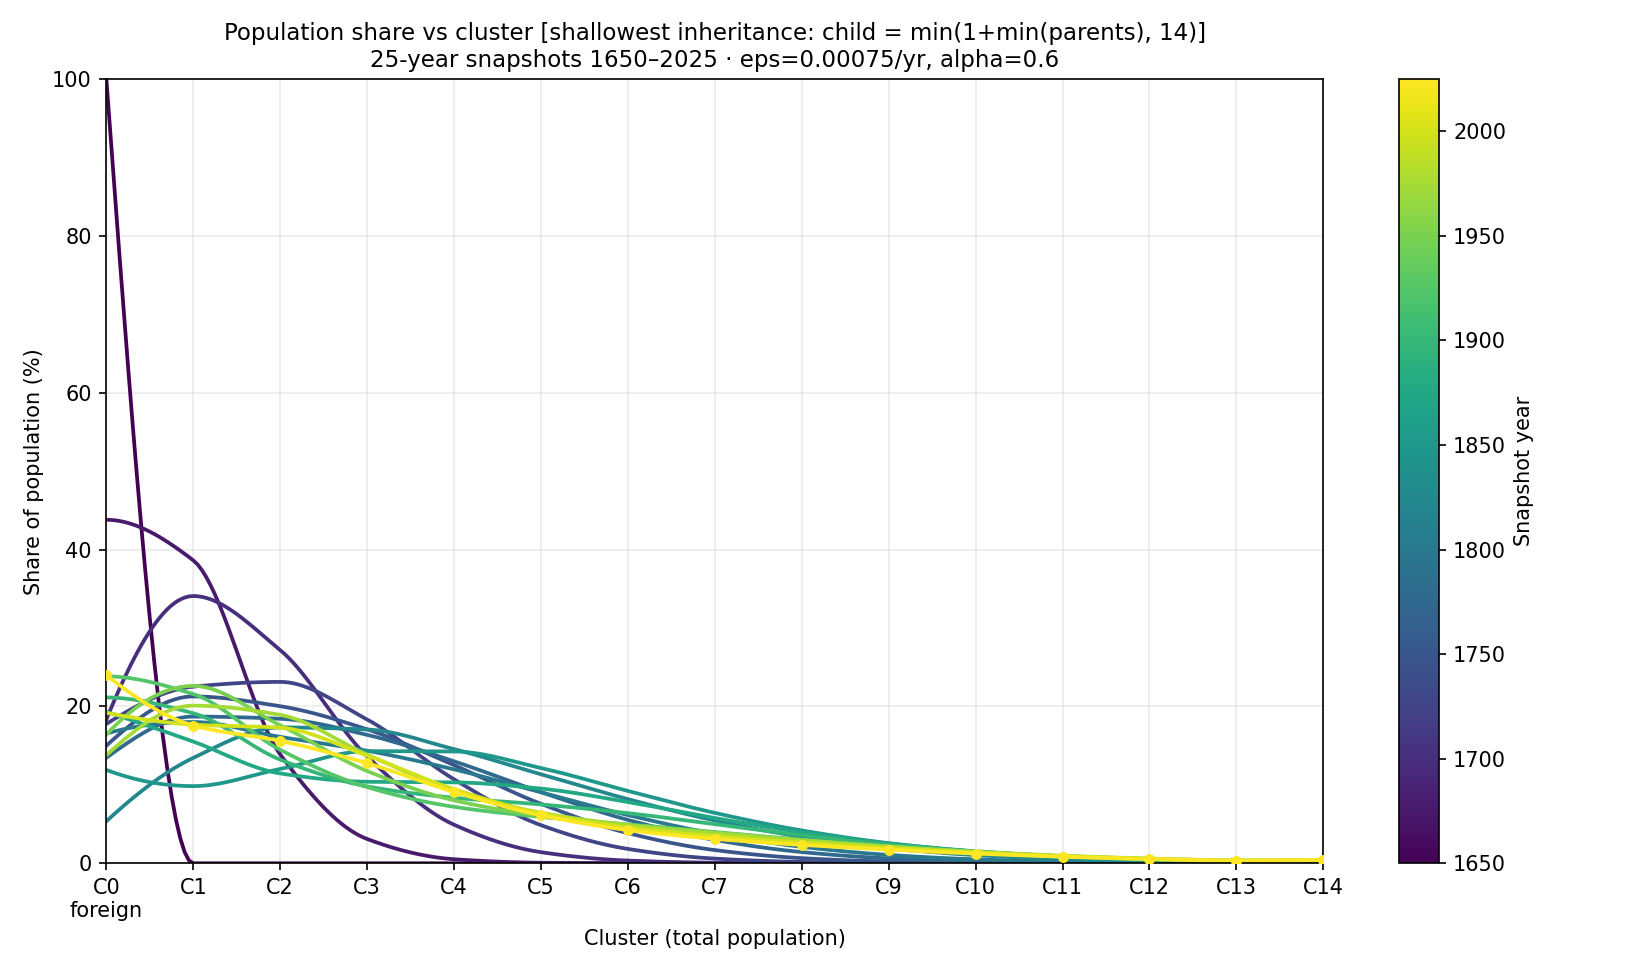
\includegraphics[width=\textwidth]{figs/dist_shallowest_inheritance_linear.png}\\
    {\scriptsize\textbf{(a) Shallowest:} $C_{14}$ = \textbf{0.45\%} by 2025 ($\alpha{=}0.8$)}
  \end{minipage}\hfill
  \begin{minipage}{0.49\textwidth}\centering
    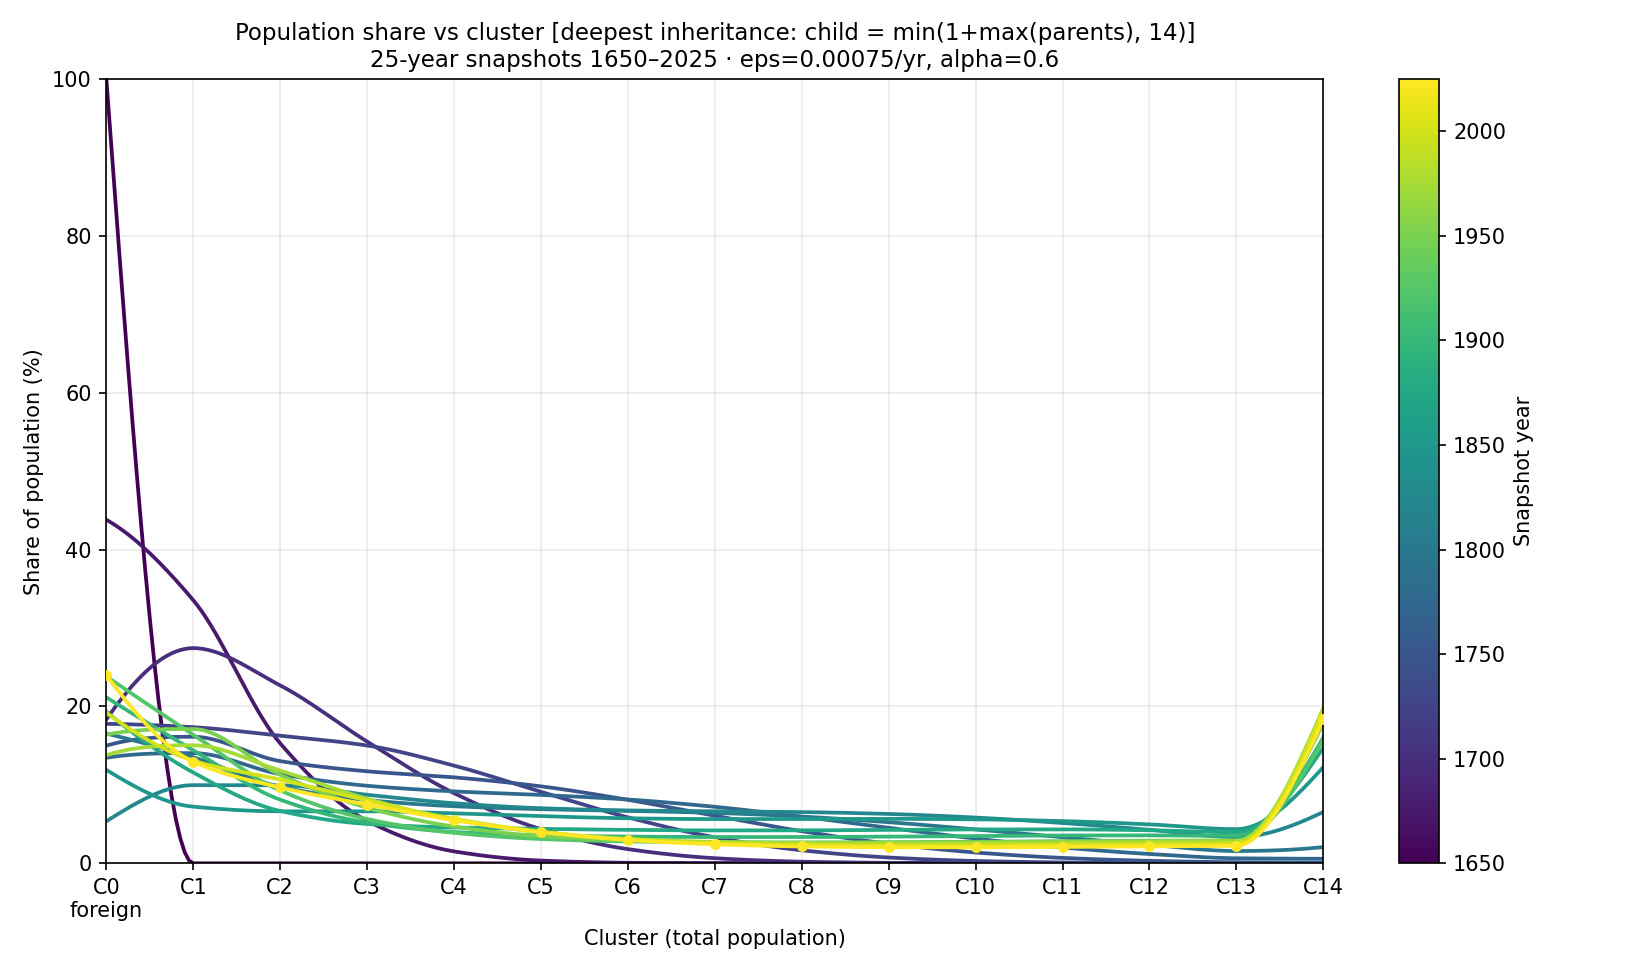
\includegraphics[width=\textwidth]{figs/dist_deepest_inheritance_linear.png}\\
    {\scriptsize\textbf{(b) Deepest:} $C_{14}$ = \textbf{18.35\%} by 2025 ($\alpha{=}0.8$)}
  \end{minipage}

  {\small 2025 $C_{14}$ share, $\alpha{=}0.0/0.8/0.9$, $n{=}14$: shallowest 0.00/\textbf{0.45}/1.46\%; deepest 71.88/\textbf{18.35}/9.44\%. Totals rule-independent (259.0\,M). \textbf{Mechanism:} shallowest pulls deep lineages down in mixed pairings; deepest never pulls down, so depth ratchets to the cap. Stronger $\alpha$ \emph{reduces} the deepest accumulation (shallow groups pair shallow).}
\end{frame}

\begin{frame}{Case 2: 2025--2050 projection}
  \centering
  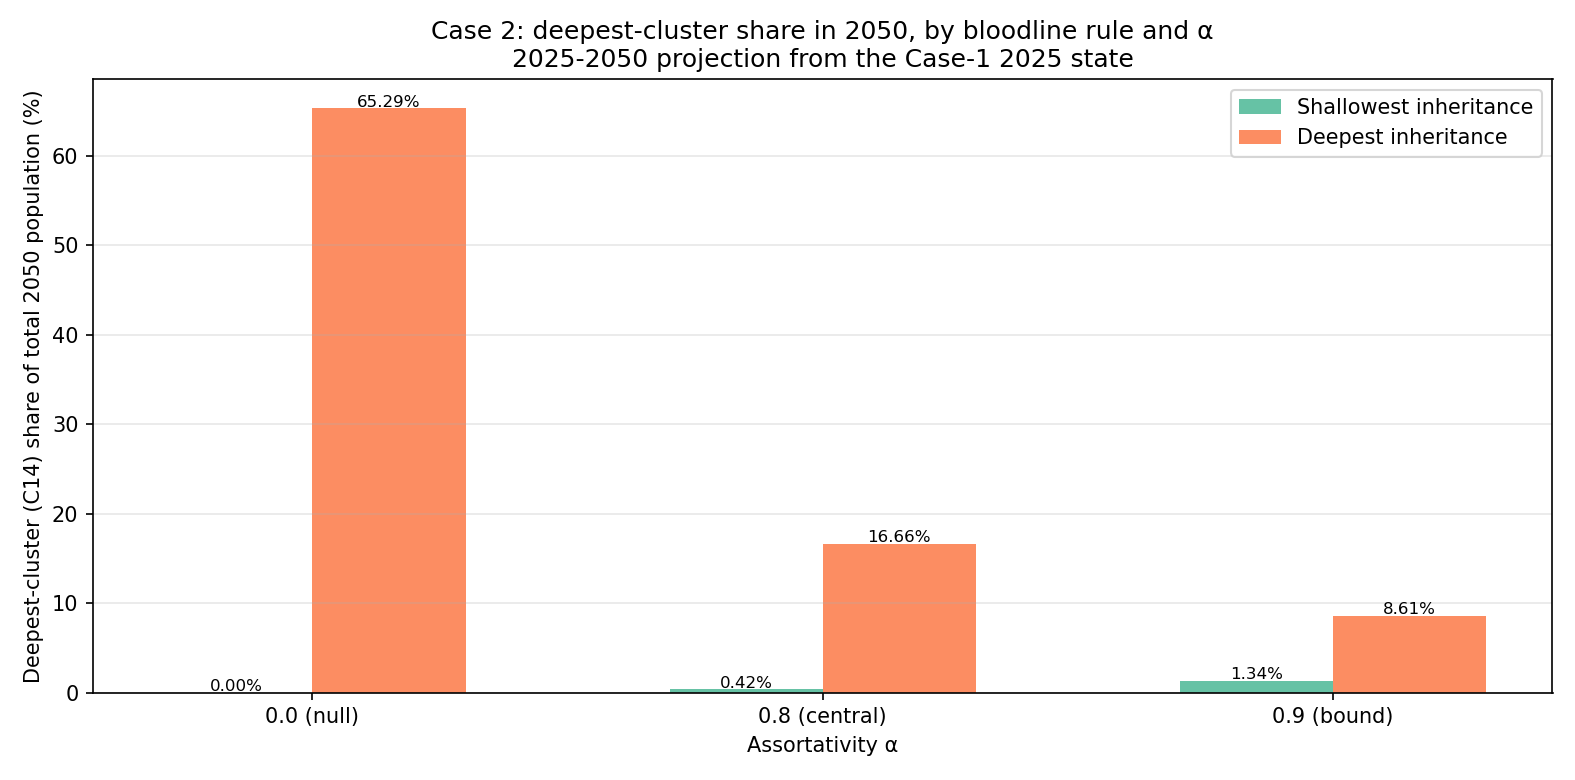
\includegraphics[width=0.62\textwidth]{figs/proj2050_cn_by_rule.png}

  {\small From the Case-1 2025 handoff state. 2050 total: \textbf{279.7\,M} (both rules). 2050 $C_{14}$ at $\alpha{=}0.8$ (2025 in parens): shallowest \textbf{0.42\%} (0.45\%); deepest \textbf{16.66\%} (18.35\%). Full 2050 $\alpha$ sweep (0.0/0.8/0.9): shallowest 0.00/0.42/1.34\%; deepest 65.29/16.66/8.61\%. Both rules dilute slightly as post-2025 immigration refreshes $C_0$ (24.0\%$\to$30.2\%). Inputs: $\beta(t)$ OLS-projected CBR, $\mu(t)$ OLS-projected CDR (excl.\ COVID), $I$ frozen at 2024, $\sigma$ held at 2024 blend (0.4703), $\varepsilon$ calibrated.}
\end{frame}

\begin{frame}{Time-varying assortativity $\alpha(t)$}
  \centering
  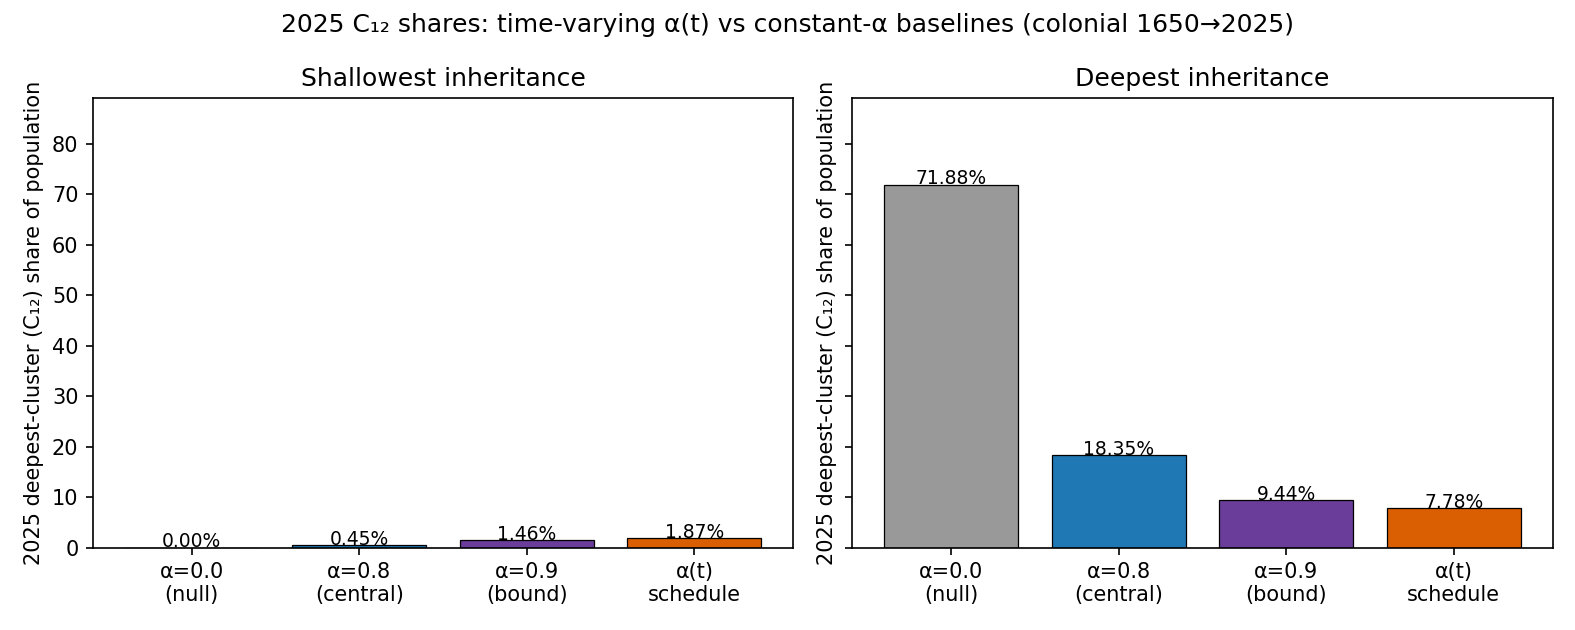
\includegraphics[width=0.88\textwidth]{figs/alpha_t_comparison.png}

  \vspace{0.5em}
  {\small The $\alpha(t)$ schedule (0.95 colonial $\to$ 0.653 in 2025, from intermarriage literature and Pew series~\cite{pew-intermarriage-2023}) gives 2025 $C_{14}$ of \textbf{1.87\%} shallowest / \textbf{7.78\%} deepest, vs 0.45\% / 18.35\% at constant $\alpha{=}0.8$. Shallowest retains path dependence (exceeds the 0.9 bound); deepest undershoots (schedule ends below 0.8 when recent mixing matters most). Sensitivity only --- constant 0.8 stays central.}\end{frame}

\begin{frame}{Sex-specific rates: the maternal bottleneck}
  \centering
  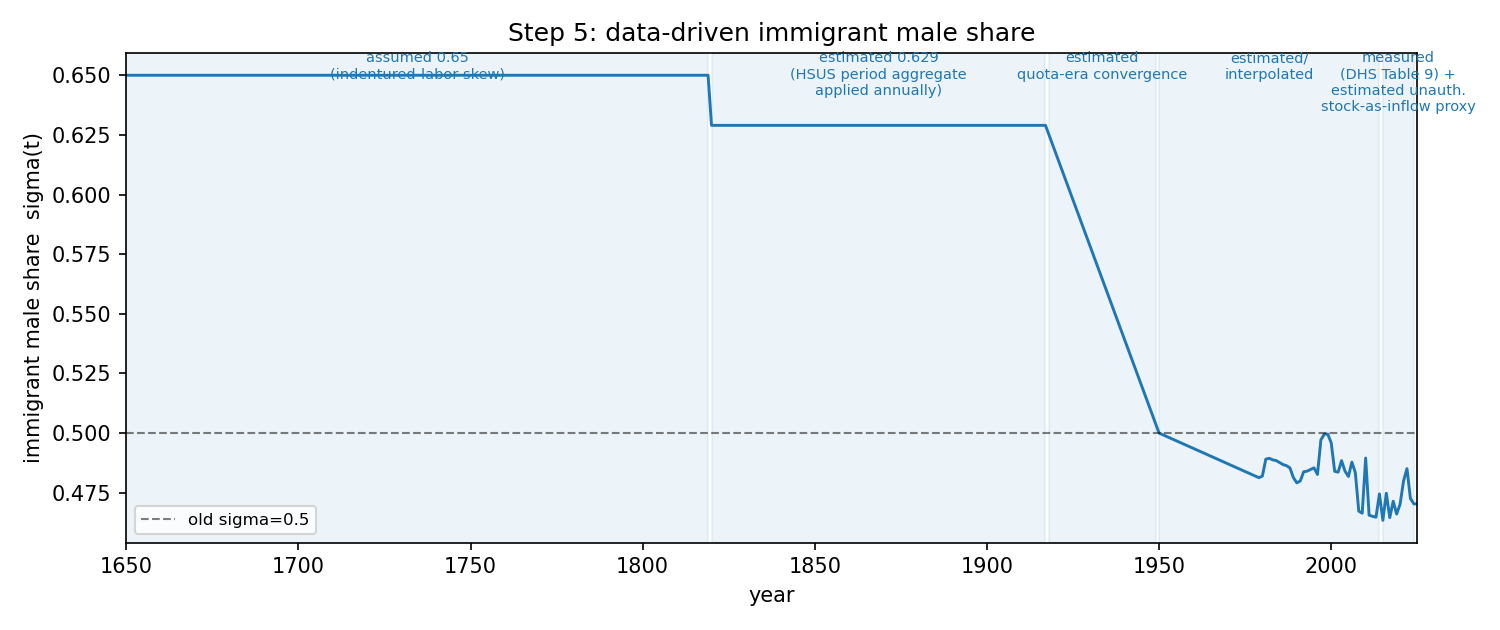
\includegraphics[width=0.82\textwidth]{figs/step5_sigma_series.png}

  {\small Immigrant male share $\sigma(t)$: 0.65 \emph{assumed} (1650--1819); 0.629 \emph{estimated} (1820--1917, HSUS~\cite{hsus-immig}); $\to$0.50 by 1950; measured DHS LPR-by-sex~\cite{dhs-lpr-sex} + unauthorized proxy~\cite{dhs-unauth-table4} from 2015. Male-skewed immigration + $\min(W^{\mathrm{pat}},W^{\mathrm{mat}})$ makes the maternal side binding: 2025 total 259.0\,M (old $\sigma$ 300.2\,M); anchor worst error $-29.3\%$ (1830) --- reported, not recalibrated. Mortality sex differential measured (HLD~\cite{hld}, 2024 $\approx 1.069$).}
\end{frame}

\begin{frame}{Depth resolution: $n{=}14$ and the bit-conserved cap}
  \centering
  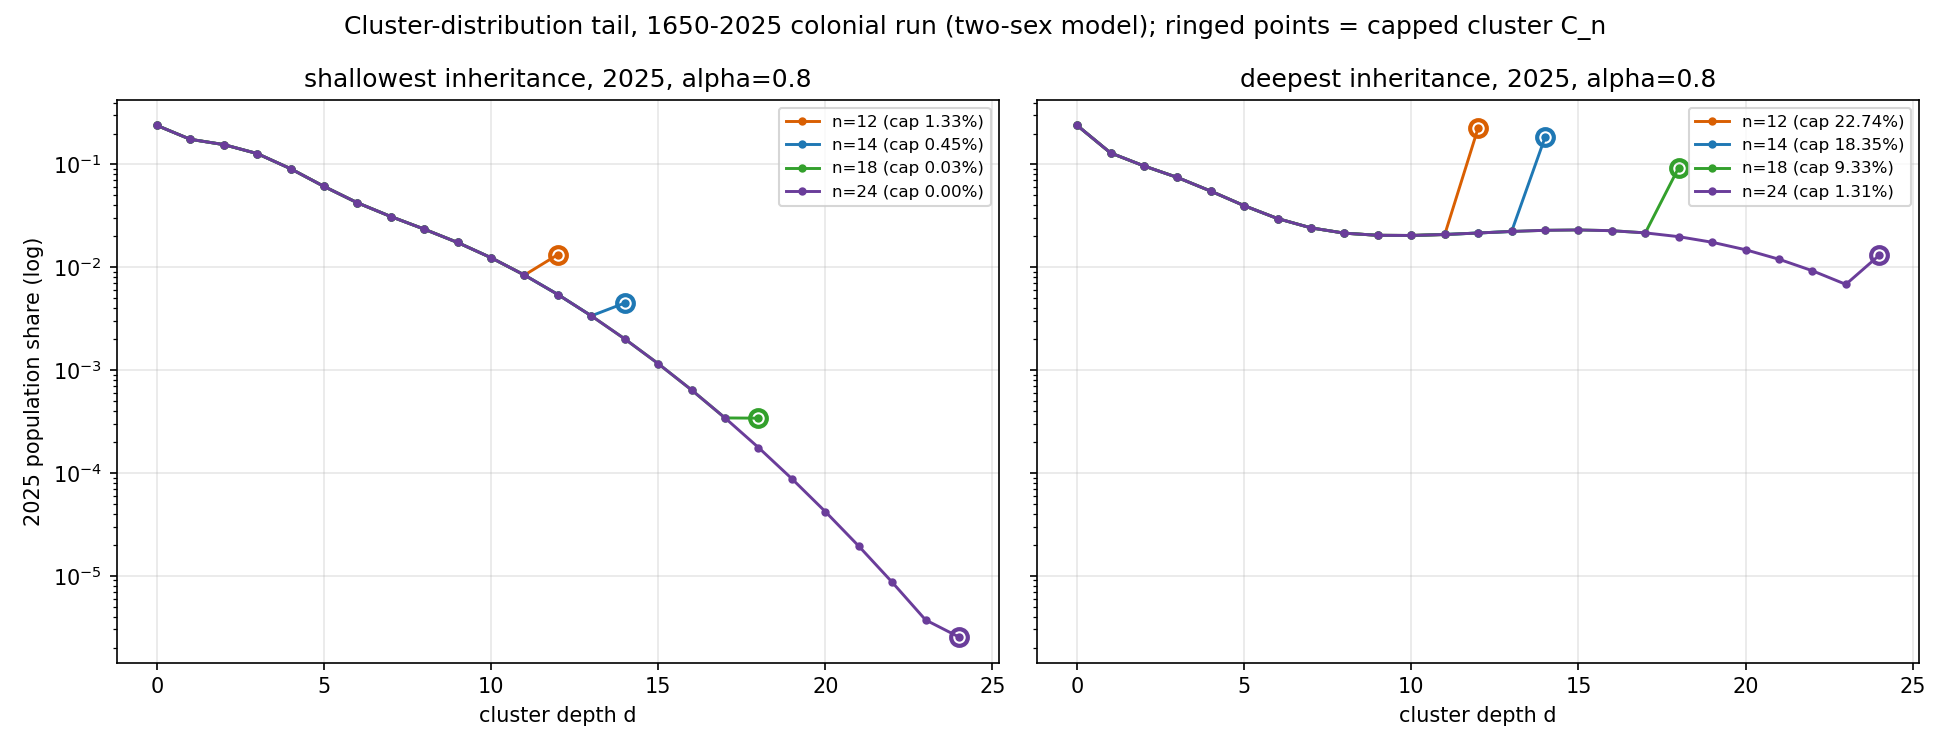
\includegraphics[width=0.85\textwidth]{figs/step6_tail_shape.png}

  \vspace{0.5em}
  {\small 2025 $C_n$ at $\alpha{=}0.8$: shallowest 1.33/{\bf0.45}/0.03/0.00\%; deepest 22.74/{\bf18.35}/9.33/1.31\% ($n{=}12/14/18/24$). Totals $n$-invariant (258.95\,M); cap bit-conserved ($C_{14} = \sum_{d\ge14}$) under both rules. Deepest cap accumulates by design (ratchet, not pile-up); $n{=}24$ resolves the tail (flat $\sim$2.2\%/cluster to $C_{17}$). $n{=}14$ is the operating point.}\end{frame}

\begin{frame}{Age structure: resolved tail nearly matches the aggregate}
  \begin{columns}
    \begin{column}{0.55\textwidth}
      \centering
      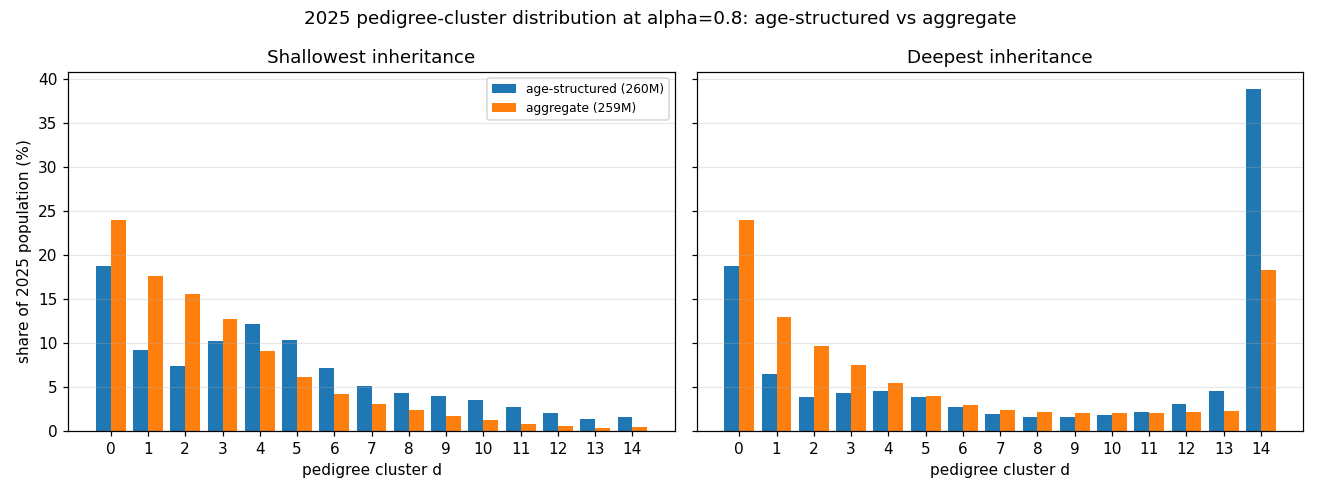
\includegraphics[width=\textwidth]{figs/cluster_dist_2025.png}
    \end{column}
    \begin{column}{0.43\textwidth}
      {\small
      \begin{itemize}
        \item 540 states: $15{\times}2{\times}18$ ($n{=}14$); aging $\gamma{=}1/5$/yr; $\sigma(t)$ series (Step 5).
        \item 2025 $C_{14}$ at $\alpha{=}0.8$: shallowest \textbf{1.62\%} vs 0.45\% agg.; deepest \textbf{38.90\%} vs 18.35\% agg. --- age structure \emph{amplifies} deep concentration, especially under deepest inheritance: older cohorts preserve a deep reservoir that the ratchet then lifts to the cap.
        \item Male-fertility sensitivity (age model): fathers $\sim$2\,yr older $\to$ 2025 $C_{14}$ $-0.8$\,pp (shallowest) to $-10$\,pp (deepest) at $\alpha{=}0.8$; totals $-4.9\%$ --- material, stays \emph{assumed}.
      \end{itemize}}
    \end{column}
  \end{columns}
\end{frame}

\begin{frame}{Generation-delay wavefront}
  \centering
  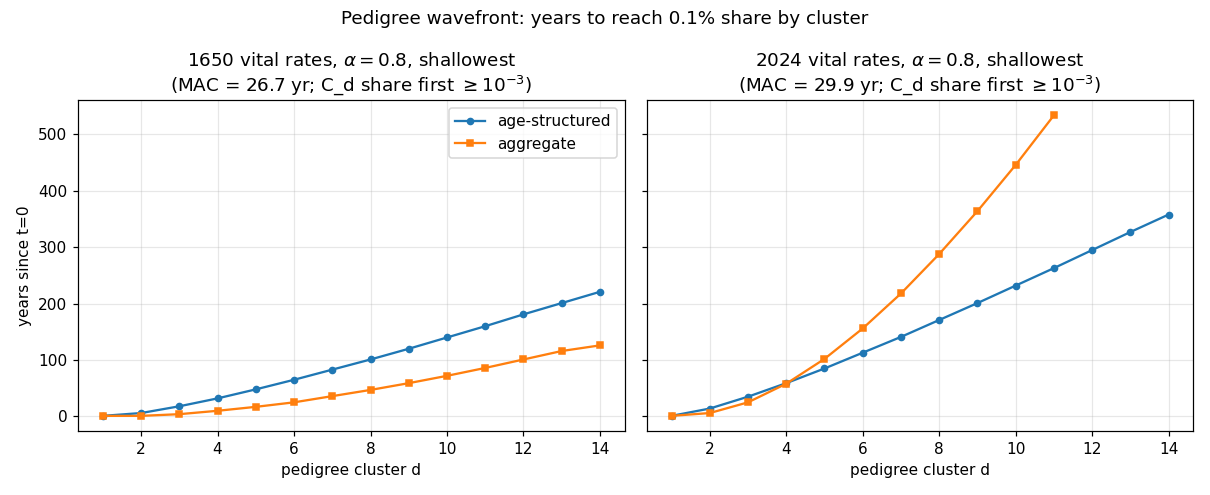
\includegraphics[width=0.88\textwidth]{figs/wavefront_comparison.png}

  {\small Years for each cluster to reach 0.1\% share (closed population, constant rates, shallowest inheritance, $\alpha=0.8$). Left (1650 rates): aggregate climbs $\approx$1.9$\times$ faster --- missing generation-delay artifact (no 15-yr parental-age floor). Right (2024 rates): aggregate is mass-accumulation-limited and runs slower. A \emph{rate} measurement, independent of $n$.}\end{frame}

\begin{frame}{Regional compartments: the Midwest runs deepest}
  \centering
  \begin{minipage}{0.58\textwidth}\centering
    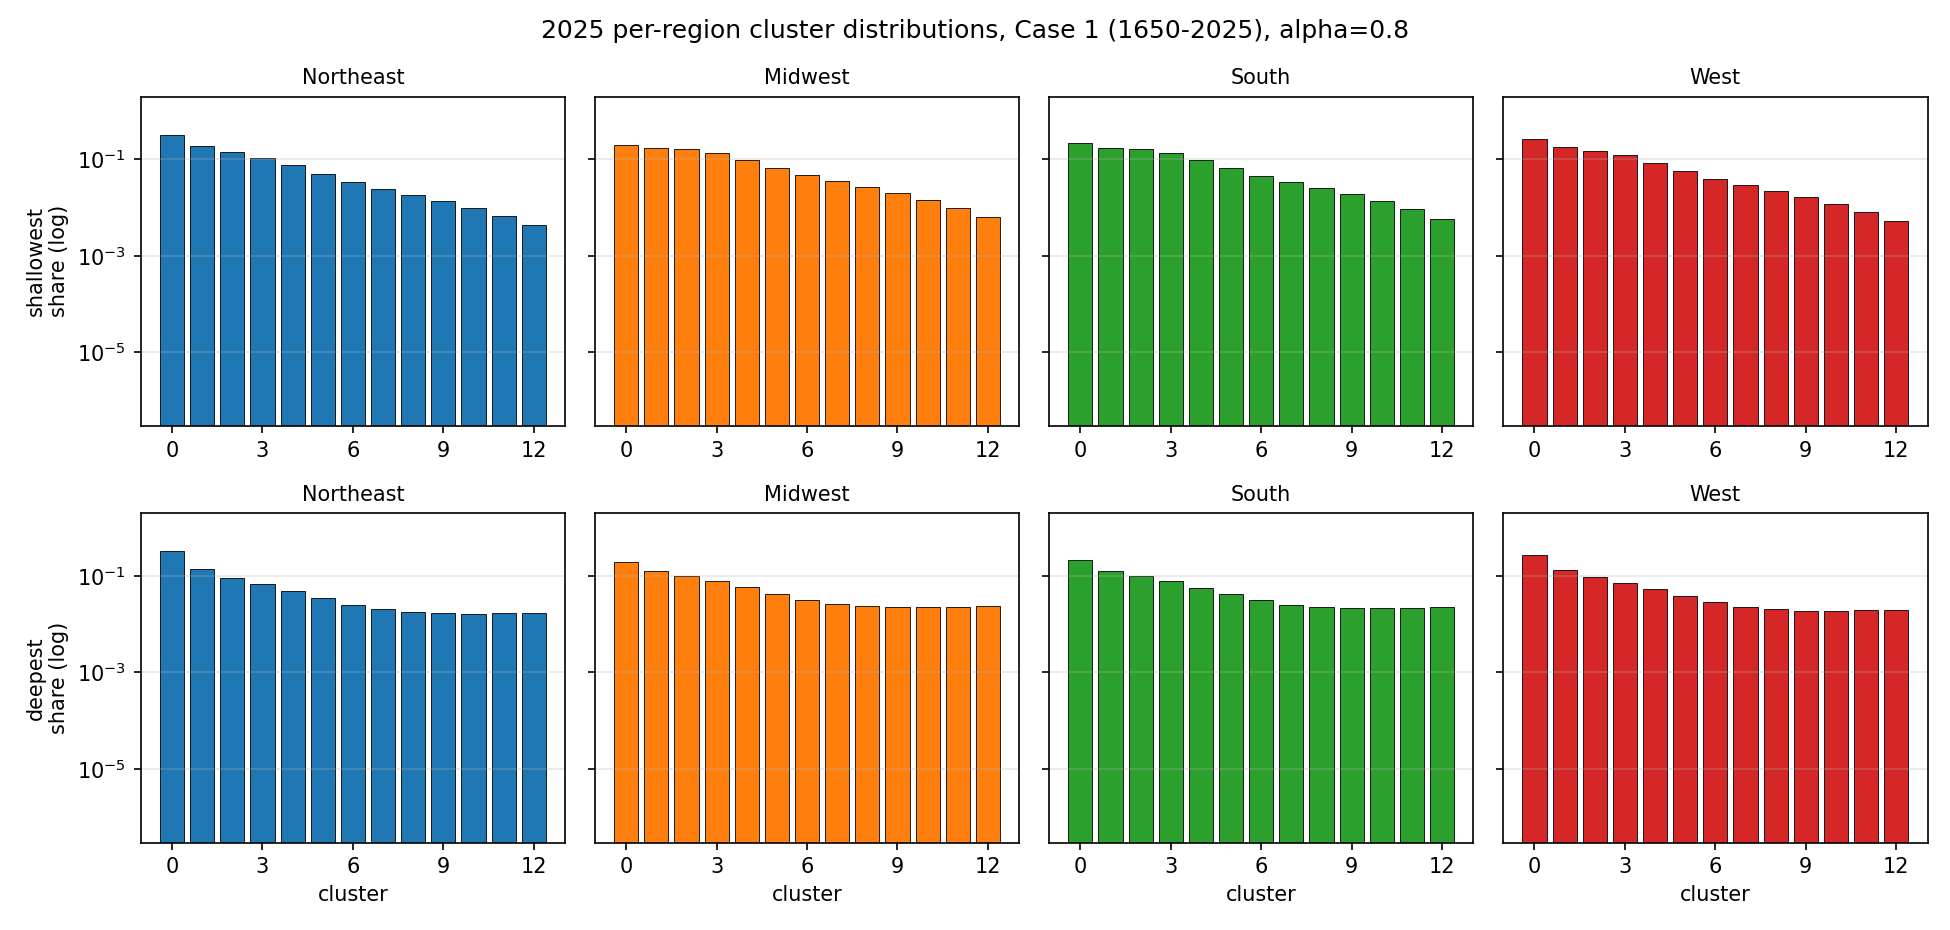
\includegraphics[width=\textwidth]{figs/regional_dist_2025.png}\\
    {\scriptsize 2025 per-region cluster distributions (Case 1, $\alpha{=}0.8$)}
  \end{minipage}\hfill
  \begin{minipage}{0.39\textwidth}\centering
    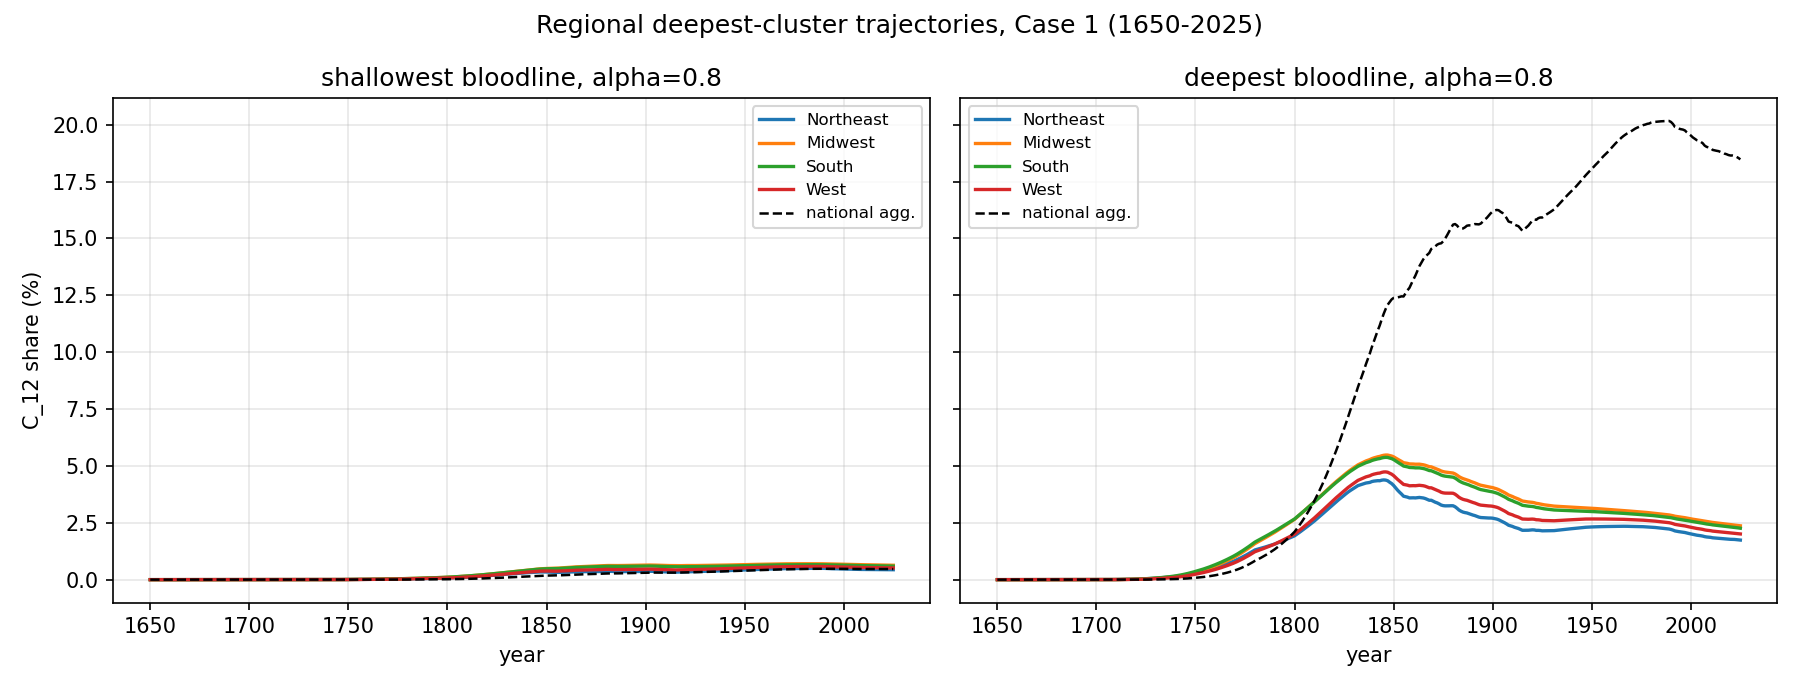
\includegraphics[width=\textwidth]{figs/regional_deepest_traj.png}\\
    {\scriptsize $C_{14}$ trajectories 1650--2025}
  \end{minipage}

  {\small 120 states, 4 Census regions; within-region mating (assumed); migration conservative. 2025 $C_{14}$ ($\alpha{=}0.8$): shallowest NE 0.36 / MW \textbf{0.53} / S 0.49 / W 0.43\%; deepest NE 14.74 / MW \textbf{20.61} / S 19.54 / W 17.20\%. Midwest deepest under both rules: smallest immigration share (11.3\%, DHS Tbl.~4~\cite{dhs-table4}) dilutes deep mass least; flows from ACS 2023--24~\cite{acs-migration}. Regional Case-2 projection in progress.}
\end{frame}

\begin{frame}{CPS parental-nativity calibration of $\alpha$}
  \centering
  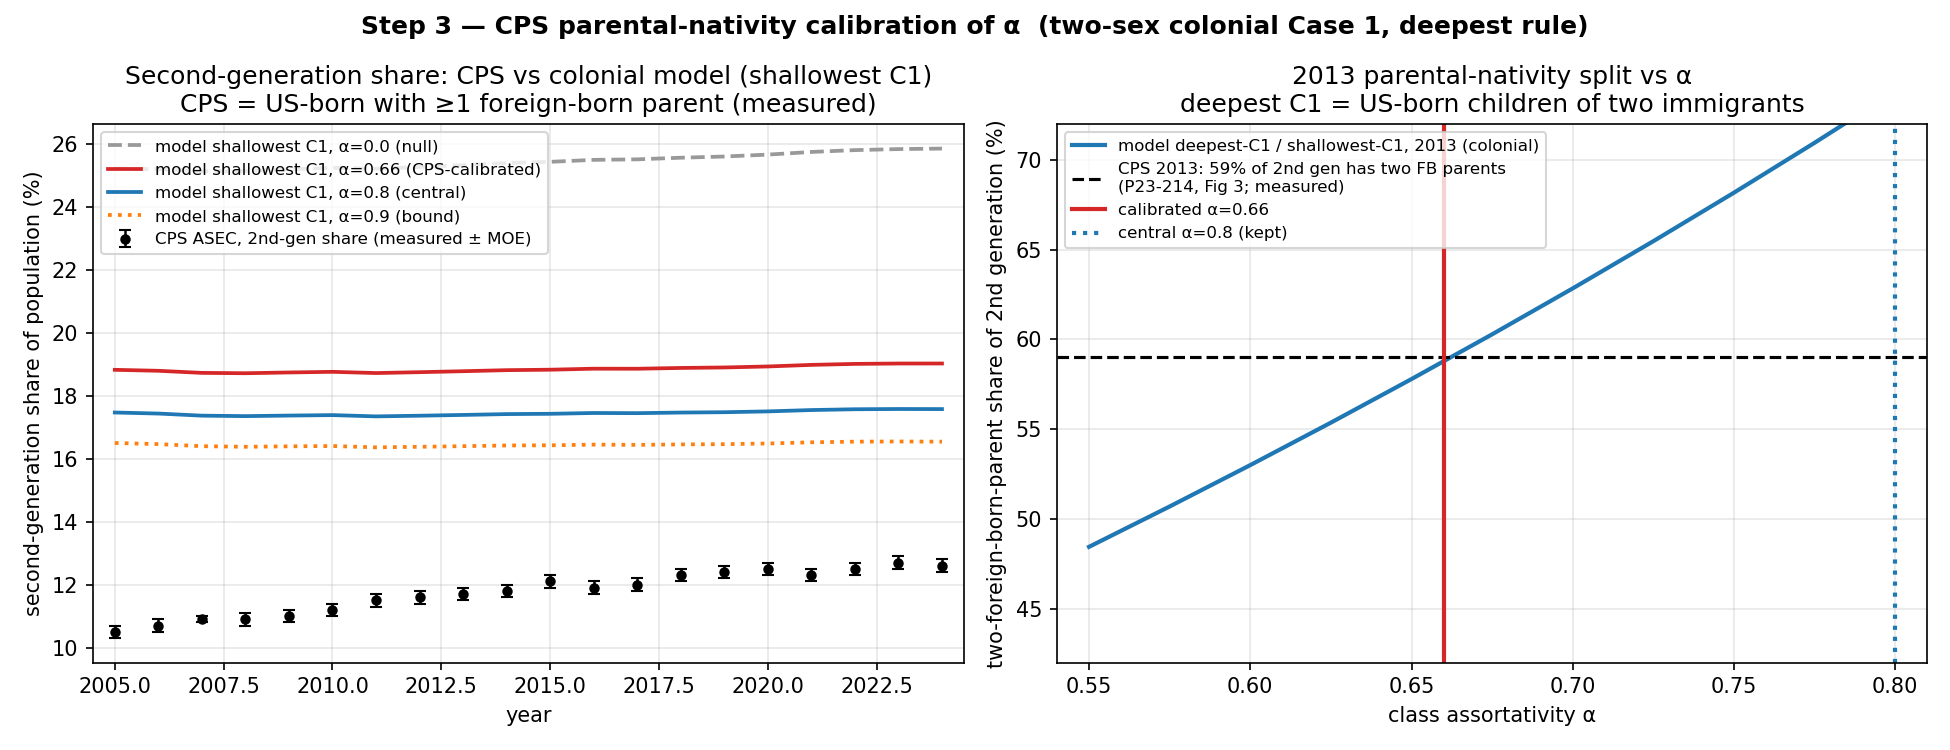
\includegraphics[width=0.85\textwidth]{figs/cps_calibration.png}

  {\small CPS ASEC 2024 Tbl.~1: second-generation share 2005--2024, 10.5\%$\to$12.6\% (measured~\cite{cps-asec-2024}); P23-214: 2013 second generation 11.7\%, 59\% with two foreign-born parents (measured~\cite{p23-214}). Model ratio deepest-$C_1$/shallowest-$C_1$ vs 59\% $\to$ $\alpha_{\mathrm{CPS}}{=}\mathbf{0.66}$; $|0.66{-}0.8|{=}0.14$ not material $\to$ keep central $\alpha{=}0.8$ (also anchored to mean religious endogamy 0.78).}
\end{frame}

\begin{frame}{Religious dimension: 8 groups, $n{=}14$}
  \centering
  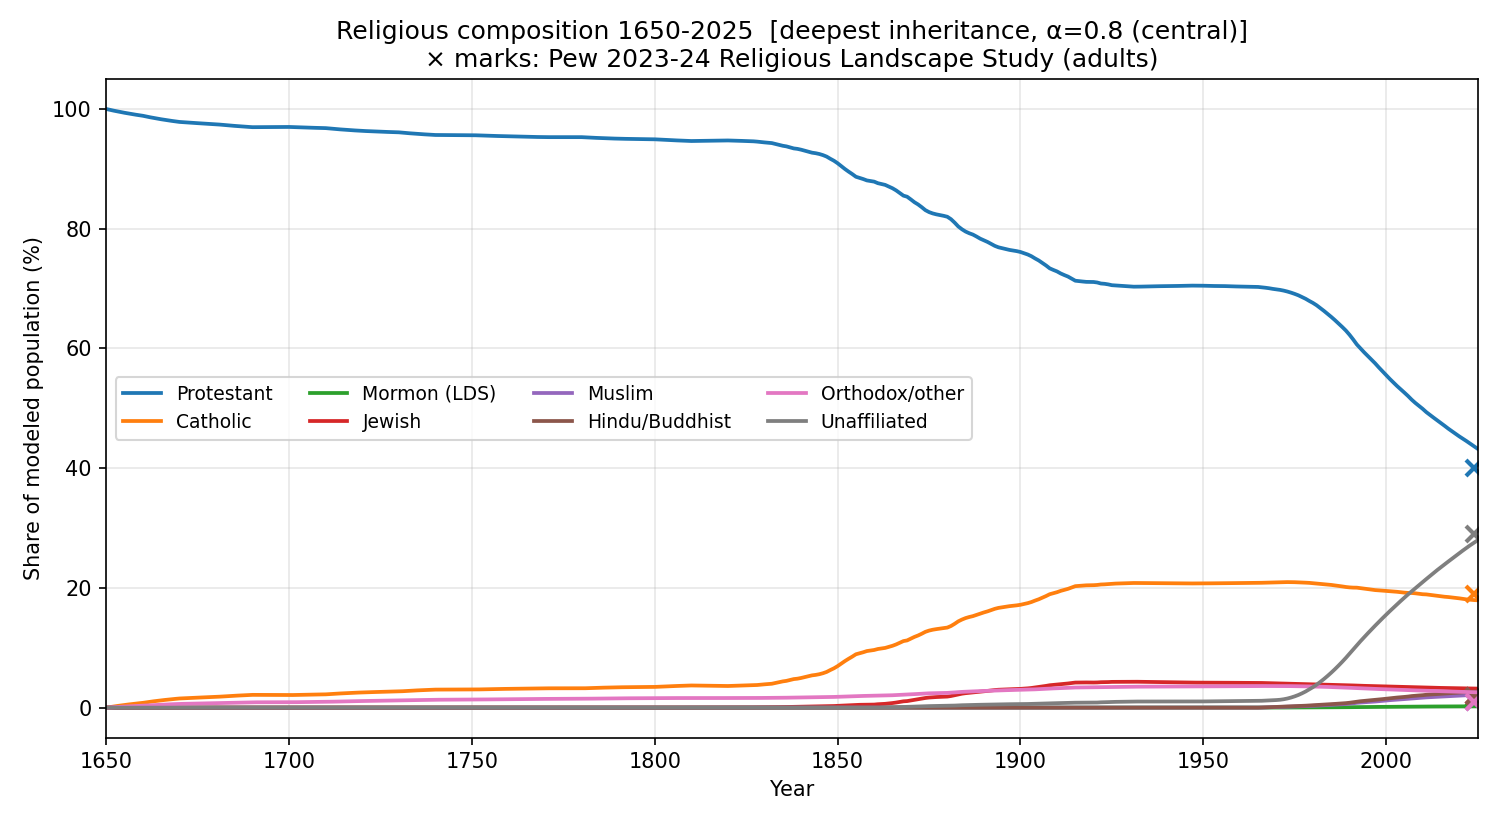
\includegraphics[width=0.88\textwidth]{figs/fig_religious_shares.png}

  {\small State $(d,s,g)$: 240 ODEs. Group endogamy $\rho_g$: mor .87, pro .81, cat .75, mus .84, jew .62, una .68 (est.\ from Pew), dhr .85, oth .80 (ass.); children take the \textbf{mother's} group (ass.). Disaffiliation ramps 1970--90 to $\delta_{\max}{=}8{\times}10^{-3}$/yr, \textbf{calibrated} to Pew unaffiliated 29\% (model 27.9\%, rule-independent). $\times$ = Pew 2023--24 RLS anchors~\cite{pew-rls-2025}. 2025 composition ($\alpha{=}0.8$, both rules): pro 43.3 / cat 17.9 / mor 0.2 / jew 3.2 / mus 2.2 / dhr 2.7 / oth 2.6 / una 27.9\%.}
\end{frame}

\begin{frame}{Deepest cluster $C_{14}$ by religious group, 2025}
  \centering
  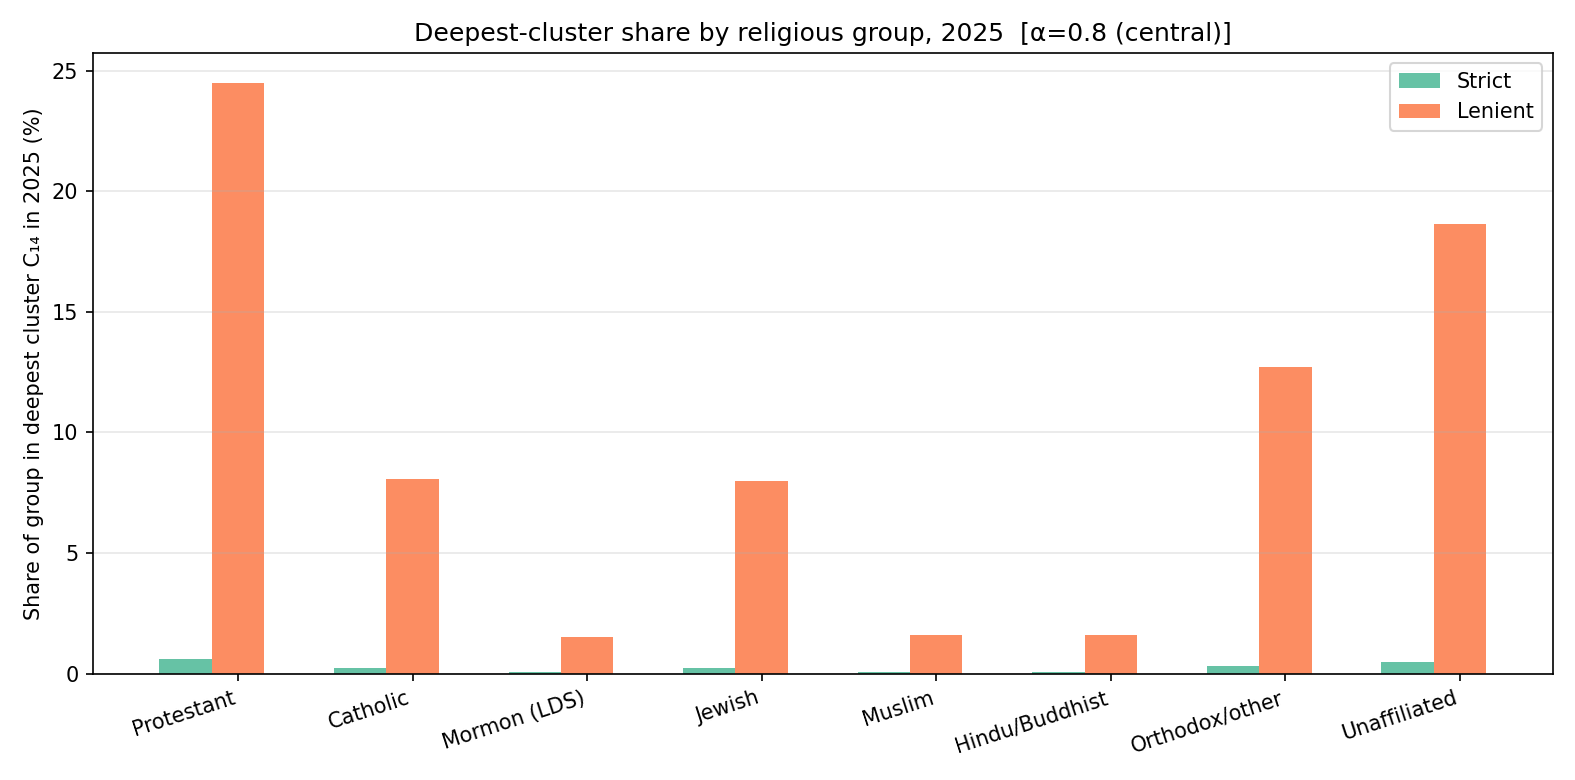
\includegraphics[width=0.88\textwidth]{figs/fig_religious_cn_by_group.png}

  {\small $C_{14}$ share of total 2025 pop.\ ($\alpha{=}0.8$, $n{=}14$): shallowest 0.45\% / deepest \textbf{17.93\%}. Demographic, not theological: long-tenure groups run deep (Protestant 24.5\%, unaffiliated 18.7\% under deepest); post-1965-immigrant groups stay shallow (Muslim, Hindu/Buddhist $\approx 1.6\%$). Under shallowest, all groups sit below 0.7\%.}
\end{frame}

\begin{frame}{Case-2 religious projection, 2025--2050}
  \centering
  {\large\color{nmgray} Run in progress under the new inheritance rules.}

  \vspace{1em}
  {\small The 2025--2050 religious projection continues disaffiliation at its calibrated rate from the Case-1 2025 handoff state. Prior pattern to retest: the unaffiliated share climbs on the one-way disaffiliation flow (a flagged artifact; two-way switching is future work).}
\end{frame}

\begin{frame}{Stochastic colonial era: the deterministic trajectory is unbiased}
  \centering
  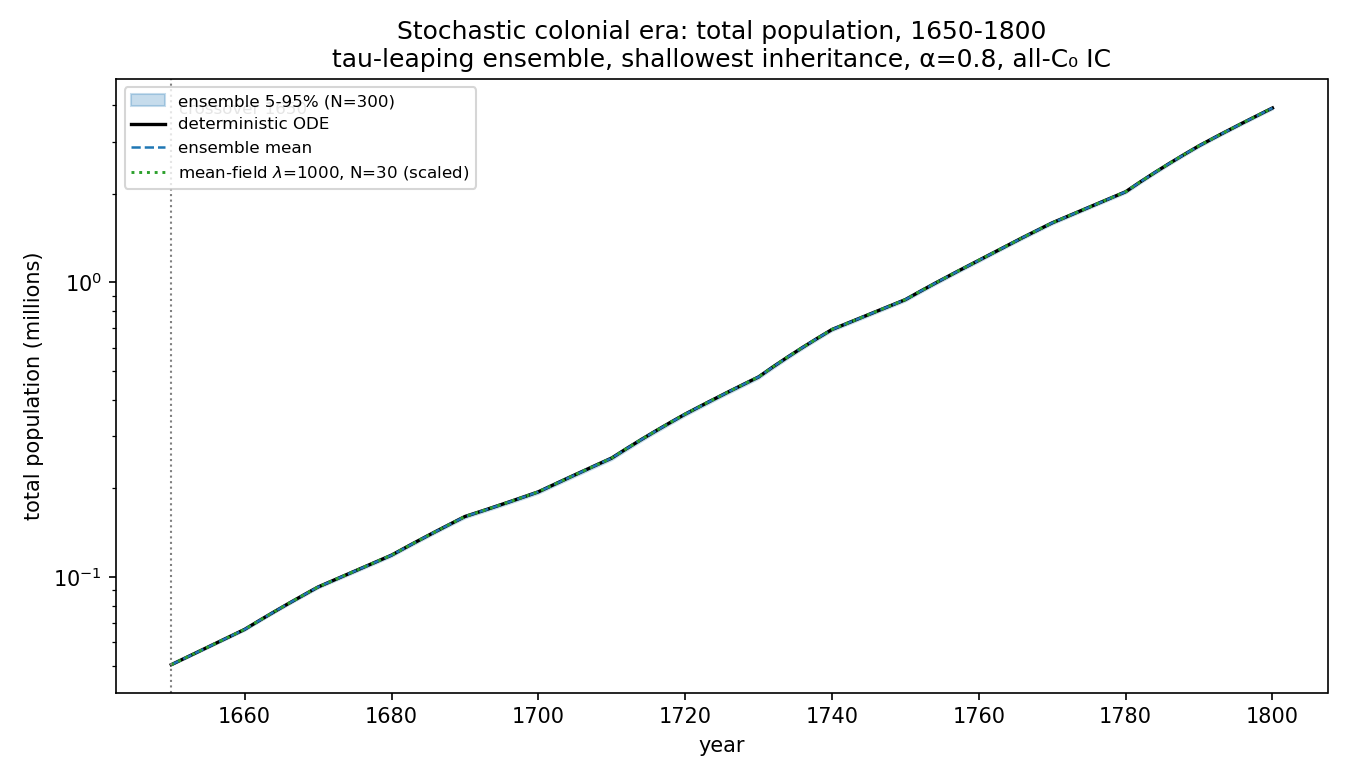
\includegraphics[width=0.8\textwidth]{figs/stochastic_fan_total.png}

  \vspace{0.5em}
  {\small
  \begin{itemize}
    \item $\tau$-leaping, $N{=}300$ traj.\ 1650--1800, both rules.
    \item No bias: $|z|\le1.40$, max dev $6.1\times10^{-4}$; mean-field check $7.7\times10^{-5}$.
    \item Deep mass robust: CV($C_{14}$) 9.5\% (shallowest) / 2.7\% (deepest) at 1800.
    \item CV(total) peaks 0.72\% $\sim$1710, never reaches 1\%; 0/300 empty $C_{12}$--$C_{14}$.
  \end{itemize}}
\end{frame}

\begin{frame}{Independent validation: rerun in progress}
  \centering
  {\large\color{nmgray} Validation checks being rerun under the new rules.}

  \vspace{1em}
  {\small
  \begin{itemize}
    \item \textbf{(a) ``American''-ancestry} (2023 ACS B04006, measured~\cite{acs-2023-b04006-b05002}): regional deep-share ranking vs observed --- prior run found a structural gap (model MW-peaked vs observed S-peaked, $\rho{=}0.60$); retesting with shallowest/deepest.
    \item \textbf{(b) Surnames:} genuine-attempt negative --- no defensible check found (2010 list~\cite{census-surnames-2010}); stands.
    \item \textbf{(c) Foreign-born} (B05002; consistency, not validation): level gap decomposition into the total bias + unauthorized accounting; rank correlation to retest.
  \end{itemize}}
\end{frame}

% ================================================================
\section{Future Work and References}
% ================================================================

\begin{frame}{Suggestions for more accurate models and data}
  \small
  \begin{enumerate}
    \item \textbf{Age $\times$ religion interaction:} the 540-state age model and 240-ODE religious model are verified unbroken but not yet combined.
    \item \textbf{Regional vital-rate differences:} regional fertility/mortality and cluster-specific migration unmodeled; regional totals uncalibrated.
    \item \textbf{Paternal age schedule:} male fertility still the female ASFR shape (assumed); a $\sim$2\,yr older paternal schedule moves 2025 $C_n$ by 2--5\,pp at $\alpha\ge0.8$; calibrate from NCHS fatherhood data.
    \item \textbf{$\alpha(t)$ for the extended models:} the time-varying assortativity schedule is two-sex only; port it to the religious, age, and regional models.
    \item \textbf{Re-affiliation in disaffiliation:} the one-way flow is an honest artifact (unaffiliated 27.9\%$\to$36.4\% by 2050); add re-affiliation.
    \item \textbf{Settlement-history process for regional deep shares:} Step 8 found a real structural gap (model peaks MW, observed ``American'' ancestry peaks S) --- add a settlement-history/identity mechanism before the regional deep ranking can be trusted.
  \end{enumerate}
\end{frame}

\begin{frame}{References}
  \tiny
  \begin{thebibliography}{9}
  \bibitem{dhs-yearbook}
  U.S.\ DHS, OHSS. \textit{Yearbook of Immigration Statistics}, Table~1 (LPRs, 1980--2024): measured $I(t)$.
  \bibitem{dhs-unauth}
  Baker, B.\ and Warren, R., OHSS, U.S.\ DHS. \textit{Estimates of the Unauthorized Immigrant Population}, various years.
  \bibitem{wdi}
  World Bank. \textit{World Development Indicators}: U.S.\ CBR/CDR, 1960--2024 ($\beta(t)$, $\mu(t)$).
  \bibitem{haines}
  Haines, M.~R. ``The Fertility Transition in the United States.'' NBER, 2002. Historical TFR/CDR anchors.
  \bibitem{census-hsus}
  U.S.\ Bureau of the Census. \textit{Historical Statistics, Colonial Times to 1970}, Ser.\ Z~1--19 (colonial anchors).
  \bibitem{census-decennial}
  U.S.\ Census Bureau. \textit{Decennial Census}, 1790--2020 (totals).
  \bibitem{nchs-natality}
  Martin, J.~A., et al. \textit{Births: Final Data for 2024.} NVSR 75(2), NCHS, 2026. Sex ratio at birth $s{=}0.512$.
  \bibitem{inputs-csv}
  Ghoniem, N.~M. \texttt{genealogy\_dynamics/data/inputs.csv}: compiled inputs, 1650--2024, with quality flags (this project).
  \bibitem{pew-rls-2025}
  Pew Research Center. \textit{Religious Landscape Study}, 2023--24. Topline + intermarriage chapter (Feb.\ 2025).
  \bibitem{pew-muslim-2017}
  Pew Research Center. \textit{U.S.\ Muslims Concerned About Their Place in Society.} July 2017 (84\% in-marriage).
  \bibitem{pew-jewish-2021}
  Pew Research Center. \textit{Jewish Americans in 2020.} May 2021 (58\% in-marriage).
  \bibitem{pew-immig-2013}
  Pew Research Center. ``The Religious Affiliation of U.S.\ Immigrants.'' May 2013 (immigrant $\iota_g$).
  \bibitem{unwpp-2024}
  UN DESA Population Division. \textit{World Population Prospects 2024}, fertility by single age, USA: ASFR for $\beta_a(t)$.
  \bibitem{hld}
  Human Life-Table Database, USA archive: $m(x)$, $L(x)$ by age/sex, 1900--2023, for $\mu_{s,a}(t)$.
  \bibitem{bell-miller}
  Bell, F.~C.\ and Miller, M.~L. \textit{Life Tables for the U.S.\ Social Security Area 1900--2100.} SSA Actuarial Study No.~116.
  \bibitem{nchs-lifetables}
  NCHS. \textit{United States Life Tables.} NVSR, annual/decennial: HLD 2001--2023; sex ratio at birth.
  \bibitem{chang1999}
  Chang, J.~T. \textit{Adv.\ Appl.\ Probab.} 31, 1002--1026 (1999): two-parent WF, genealogical MRCA $\sim\!\log_2 n$.
  \bibitem{rohde2004}
  Rohde, Olson \& Chang. \textit{Nature} 431, 562--566 (2004): recent common ancestry under substructure.
  \bibitem{derrida1999}
  Derrida, Manrubia \& Zanette. \textit{Phys.\ Rev.\ Lett.} 82, 1987--1990 (1999): genealogical-tree statistics.
  \bibitem{derrida2000}
  Derrida, Manrubia \& Zanette. \textit{J.\ Theor.\ Biol.} 203, 303--315 (2000): biparental pedigree collapse.
  \bibitem{manrubia2002}
  Manrubia \& Zanette. \textit{J.\ Theor.\ Biol.} 216, 461--477 (2002): birth--death model of surname transmission.
  \bibitem{cavalli-sforza1981}
  Cavalli-Sforza \& Feldman. \textit{Cultural Transmission and Evolution.} Princeton UP (1981).
  \bibitem{matsen2008}
  Matsen \& Evans. \textit{Theor.\ Popul.\ Biol.} 74, 182--190 (2008): genealogical $\ne$ genetic ancestry.
  \end{thebibliography}
\end{frame}

\begin{frame}[shrink]{References (cont.)}
  \tiny
  \begin{thebibliography}{9}
  \bibitem{acs-migration}
  U.S.\ Census Bureau. ACS 1-year state-to-state migration flows, 2023--2024.
  \bibitem{dhs-table4}
  U.S.\ DHS, OHSS. \textit{Yearbook 2023}, Table~4: LPRs by state, FY2014--2023.
  \bibitem{cps-asec-2024}
  U.S.\ Census Bureau. CPS 2024 ASEC, Foreign-Born Table~1: population by generation, 2005--2024.
  \bibitem{p23-214}
  Trevelyan et~al. \textit{Characteristics of the U.S.\ Population by Generational Status: 2013.} P23-214, 2016.
  \bibitem{pew-intermarriage}
  Pew Research Center. ``Interracial Marriage Grows,'' June 15, 2023; Livingston \& Brown, ``Intermarriage in the U.S.\ 50 Years After \textit{Loving v.\ Virginia},'' May 18, 2017.
  \bibitem{alba-anchors}
  Alba \& Golden, ``Patterns of Ethnic Marriage in the United States,'' \textit{Social Forces} 65(1), 1986; Alba, \textit{Italian Americans}, Prentice-Hall, 1983.
  \bibitem{endogamy-1880}
  Sp\"orlein et~al., 2014; Logan \& Shin, ``Assimilation by the Third Generation?,'' \textit{IMR} 46(3), 2012.
  \bibitem{endogamy-1910}
  Pagnini \& Morgan, ``Intermarriage and Social Distance,'' \textit{AJS} 96(2), 1990; Draschler, \textit{Intermarriage in New York City}, Columbia UP, 1921.
  \bibitem{hsus-immig}
  \textit{Historical Statistics of the U.S.}, Millennial Ed.: Aa essay (62.9\% male, 1820--1917); Ad essay (parity by 1950).
  \bibitem{dhs-lpr-sex}
  U.S.\ DHS, OHSS. \textit{Yearbook}, Table~9: LPR admissions by sex, 2015--2023.
  \bibitem{dhs-unauth-table4}
  U.S.\ DHS, OHSS. Unauthorized-immigrant estimates, Table~4 (sex composition).
  \bibitem{gillespie-1976}
  Gillespie, D.~T. \textit{J.\ Comput.\ Phys.} 22(4), 403--434, 1976: exact SSA (the simulated jump process).
  \bibitem{gillespie-2001}
  Gillespie, D.~T. \textit{J.\ Chem.\ Phys.} 115(4), 1716--1733, 2001: $\tau$-leaping.
  \bibitem{cao-gillespie-petzold-2006}
  Cao, Y., Gillespie, D.~T.\ and Petzold, L.~R. \textit{J.\ Chem.\ Phys.} 124(4), 044109, 2006: adaptive $\tau$.
  \bibitem{kurtz-1970}
  Kurtz, T.~G. \textit{J.\ Appl.\ Probab.} 7(1), 49--58, 1970: mean-field limit (jump process $\to$ ODE).
  \bibitem{acs-2023-b04006-b05002}
  U.S.\ Census Bureau. 2023 ACS 1-year, Tables B04006/B05002, table-based summary files, accessed 2026-09-26.
  \bibitem{census-surnames-2010}
  U.S.\ Census Bureau. 2010 Census surnames, \texttt{Names\_2010Census.csv}, accessed 2026-09-26 (no defensible check found).
  \end{thebibliography}
\end{frame}

\begin{frame}
  \vfill
  \centering
  {\Large\bfseries\color{nmblue} Thank you}
  \vfill
\end{frame}

\end{document}
